\documentclass[twoside]{book}

% Packages required by doxygen
\usepackage{calc}
\usepackage{doxygen}
\usepackage{graphicx}
\usepackage[utf8]{inputenc}
\usepackage{makeidx}
\usepackage{multicol}
\usepackage{multirow}
\usepackage{textcomp}
\usepackage[table]{xcolor}

% Font selection
\usepackage[T1]{fontenc}
\usepackage{mathptmx}
\usepackage[scaled=.90]{helvet}
\usepackage{courier}
\usepackage{amssymb}
\usepackage{sectsty}
\renewcommand{\familydefault}{\sfdefault}
\allsectionsfont{%
  \fontseries{bc}\selectfont%
  \color{darkgray}%
}
\renewcommand{\DoxyLabelFont}{%
  \fontseries{bc}\selectfont%
  \color{darkgray}%
}

% Page & text layout
\usepackage{geometry}
\geometry{%
  a4paper,%
  top=2.5cm,%
  bottom=2.5cm,%
  left=2.5cm,%
  right=2.5cm%
}
\tolerance=750
\hfuzz=15pt
\hbadness=750
\setlength{\emergencystretch}{15pt}
\setlength{\parindent}{0cm}
\setlength{\parskip}{0.2cm}
\makeatletter
\renewcommand{\paragraph}{%
  \@startsection{paragraph}{4}{0ex}{-1.0ex}{1.0ex}{%
    \normalfont\normalsize\bfseries\SS@parafont%
  }%
}
\renewcommand{\subparagraph}{%
  \@startsection{subparagraph}{5}{0ex}{-1.0ex}{1.0ex}{%
    \normalfont\normalsize\bfseries\SS@subparafont%
  }%
}
\makeatother

% Headers & footers
\usepackage{fancyhdr}
\pagestyle{fancyplain}
\fancyhead[LE]{\fancyplain{}{\bfseries\thepage}}
\fancyhead[CE]{\fancyplain{}{}}
\fancyhead[RE]{\fancyplain{}{\bfseries\leftmark}}
\fancyhead[LO]{\fancyplain{}{\bfseries\rightmark}}
\fancyhead[CO]{\fancyplain{}{}}
\fancyhead[RO]{\fancyplain{}{\bfseries\thepage}}
\fancyfoot[LE]{\fancyplain{}{}}
\fancyfoot[CE]{\fancyplain{}{}}
\fancyfoot[RE]{\fancyplain{}{\bfseries\scriptsize Generated on Tue Dec 17 2013 12\-:12\-:37 for tshark by Doxygen }}
\fancyfoot[LO]{\fancyplain{}{\bfseries\scriptsize Generated on Tue Dec 17 2013 12\-:12\-:37 for tshark by Doxygen }}
\fancyfoot[CO]{\fancyplain{}{}}
\fancyfoot[RO]{\fancyplain{}{}}
\renewcommand{\footrulewidth}{0.4pt}
\renewcommand{\chaptermark}[1]{%
  \markboth{#1}{}%
}
\renewcommand{\sectionmark}[1]{%
  \markright{\thesection\ #1}%
}

% Indices & bibliography
\usepackage{natbib}
\usepackage[titles]{tocloft}
\setcounter{tocdepth}{3}
\setcounter{secnumdepth}{5}
\makeindex

% Hyperlinks (required, but should be loaded last)
\usepackage{ifpdf}
\ifpdf
  \usepackage[pdftex,pagebackref=true]{hyperref}
\else
  \usepackage[ps2pdf,pagebackref=true]{hyperref}
\fi
\hypersetup{%
  colorlinks=true,%
  linkcolor=blue,%
  citecolor=blue,%
  unicode%
}

% Custom commands
\newcommand{\clearemptydoublepage}{%
  \newpage{\pagestyle{empty}\cleardoublepage}%
}


%===== C O N T E N T S =====

\begin{document}

% Titlepage & ToC
\hypersetup{pageanchor=false}
\pagenumbering{roman}
\begin{titlepage}
\vspace*{7cm}
\begin{center}%
{\Large tshark }\\
\vspace*{1cm}
{\large Generated by Doxygen 1.8.5}\\
\vspace*{0.5cm}
{\small Tue Dec 17 2013 12:12:37}\\
\end{center}
\end{titlepage}
\clearemptydoublepage
\tableofcontents
\clearemptydoublepage
\pagenumbering{arabic}
\hypersetup{pageanchor=true}

%--- Begin generated contents ---
\chapter{Namespace Index}
\section{Packages}
Here are the packages with brief descriptions (if available)\-:\begin{DoxyCompactList}
\item\contentsline{section}{\hyperlink{namespaceabbas__to__arash}{abbas\-\_\-to\-\_\-arash} }{\pageref{namespaceabbas__to__arash}}{}
\item\contentsline{section}{\hyperlink{namespaceabbas__to__arash2}{abbas\-\_\-to\-\_\-arash2} }{\pageref{namespaceabbas__to__arash2}}{}
\item\contentsline{section}{\hyperlink{namespaceadd__timestamp}{add\-\_\-timestamp} }{\pageref{namespaceadd__timestamp}}{}
\item\contentsline{section}{\hyperlink{namespacecdf}{cdf} }{\pageref{namespacecdf}}{}
\item\contentsline{section}{\hyperlink{namespacecompare__comms}{compare\-\_\-comms} }{\pageref{namespacecompare__comms}}{}
\item\contentsline{section}{\hyperlink{namespaceexcess__code}{excess\-\_\-code} }{\pageref{namespaceexcess__code}}{}
\item\contentsline{section}{\hyperlink{namespaceget__all__pairs}{get\-\_\-all\-\_\-pairs} }{\pageref{namespaceget__all__pairs}}{}
\item\contentsline{section}{\hyperlink{namespaceks2}{ks2} }{\pageref{namespaceks2}}{}
\item\contentsline{section}{\hyperlink{namespacepython__lib}{python\-\_\-lib} }{\pageref{namespacepython__lib}}{}
\item\contentsline{section}{\hyperlink{namespacescapy__parser}{scapy\-\_\-parser} }{\pageref{namespacescapy__parser}}{}
\item\contentsline{section}{\hyperlink{namespacetcp__client}{tcp\-\_\-client} }{\pageref{namespacetcp__client}}{}
\item\contentsline{section}{\hyperlink{namespacetcp__server}{tcp\-\_\-server} }{\pageref{namespacetcp__server}}{}
\item\contentsline{section}{\hyperlink{namespacetemplate}{template} }{\pageref{namespacetemplate}}{}
\item\contentsline{section}{\hyperlink{namespacethrouput__tshark}{throuput\-\_\-tshark} }{\pageref{namespacethrouput__tshark}}{}
\item\contentsline{section}{\hyperlink{namespacetornado__server}{tornado\-\_\-server} }{\pageref{namespacetornado__server}}{}
\item\contentsline{section}{\hyperlink{namespacevpn__no__vpn}{vpn\-\_\-no\-\_\-vpn} }{\pageref{namespacevpn__no__vpn}}{}
\item\contentsline{section}{\hyperlink{namespacewrapper__client}{wrapper\-\_\-client} }{\pageref{namespacewrapper__client}}{}
\item\contentsline{section}{\hyperlink{namespacewrapper__server}{wrapper\-\_\-server} }{\pageref{namespacewrapper__server}}{}
\end{DoxyCompactList}

\chapter{Hierarchical Index}
\section{Class Hierarchy}
This inheritance list is sorted roughly, but not completely, alphabetically\-:\begin{DoxyCompactList}
\item object\begin{DoxyCompactList}
\item \contentsline{section}{cdf.\-Data\-Point}{\pageref{classcdf_1_1_data_point}}{}
\item \contentsline{section}{cdf.\-Dump\-Stat}{\pageref{classcdf_1_1_dump_stat}}{}
\item \contentsline{section}{ks2.\-Data\-Point}{\pageref{classks2_1_1_data_point}}{}
\item \contentsline{section}{ks2.\-Dump\-Stat}{\pageref{classks2_1_1_dump_stat}}{}
\item \contentsline{section}{python\-\_\-lib.\-Configs}{\pageref{classpython__lib_1_1_configs}}{}
\item \contentsline{section}{python\-\_\-lib.\-Instance}{\pageref{classpython__lib_1_1_instance}}{}
\item \contentsline{section}{python\-\_\-lib.\-One\-Response}{\pageref{classpython__lib_1_1_one_response}}{}
\item \contentsline{section}{python\-\_\-lib.\-Request\-Set}{\pageref{classpython__lib_1_1_request_set}}{}
\item \contentsline{section}{python\-\_\-lib.\-Response\-Set}{\pageref{classpython__lib_1_1_response_set}}{}
\item \contentsline{section}{tcp\-\_\-client.\-Connections}{\pageref{classtcp__client_1_1_connections}}{}
\item \contentsline{section}{tcp\-\_\-client.\-Queue}{\pageref{classtcp__client_1_1_queue}}{}
\item \contentsline{section}{tcp\-\_\-client.\-Send\-Recv}{\pageref{classtcp__client_1_1_send_recv}}{}
\item \contentsline{section}{tcp\-\_\-server.\-Server}{\pageref{classtcp__server_1_1_server}}{}
\item \contentsline{section}{throuput\-\_\-tshark.\-Data\-Point}{\pageref{classthrouput__tshark_1_1_data_point}}{}
\item \contentsline{section}{throuput\-\_\-tshark.\-Dump\-Stat}{\pageref{classthrouput__tshark_1_1_dump_stat}}{}
\item \contentsline{section}{vpn\-\_\-no\-\_\-vpn.\-tcpdump}{\pageref{classvpn__no__vpn_1_1tcpdump}}{}
\end{DoxyCompactList}
\item Request\-Handler\begin{DoxyCompactList}
\item \contentsline{section}{tornado\-\_\-server.\-Main\-Handler}{\pageref{classtornado__server_1_1_main_handler}}{}
\item \contentsline{section}{tornado\-\_\-server.\-Record\-Replay}{\pageref{classtornado__server_1_1_record_replay}}{}
\item \contentsline{section}{tornado\-\_\-server.\-Re\-Run}{\pageref{classtornado__server_1_1_re_run}}{}
\end{DoxyCompactList}
\item type\begin{DoxyCompactList}
\item \contentsline{section}{python\-\_\-lib.\-Singleton}{\pageref{classpython__lib_1_1_singleton}}{}
\end{DoxyCompactList}
\end{DoxyCompactList}

\chapter{Class Index}
\section{Class List}
Here are the classes, structs, unions and interfaces with brief descriptions\-:\begin{DoxyCompactList}
\item\contentsline{section}{\hyperlink{classpython__lib_1_1_configs}{python\-\_\-lib.\-Configs} }{\pageref{classpython__lib_1_1_configs}}{}
\item\contentsline{section}{\hyperlink{classtcp__client_1_1_connections}{tcp\-\_\-client.\-Connections} }{\pageref{classtcp__client_1_1_connections}}{}
\item\contentsline{section}{\hyperlink{classcdf_1_1_data_point}{cdf.\-Data\-Point} }{\pageref{classcdf_1_1_data_point}}{}
\item\contentsline{section}{\hyperlink{classks2_1_1_data_point}{ks2.\-Data\-Point} }{\pageref{classks2_1_1_data_point}}{}
\item\contentsline{section}{\hyperlink{classthrouput__tshark_1_1_data_point}{throuput\-\_\-tshark.\-Data\-Point} }{\pageref{classthrouput__tshark_1_1_data_point}}{}
\item\contentsline{section}{\hyperlink{classcdf_1_1_dump_stat}{cdf.\-Dump\-Stat} }{\pageref{classcdf_1_1_dump_stat}}{}
\item\contentsline{section}{\hyperlink{classthrouput__tshark_1_1_dump_stat}{throuput\-\_\-tshark.\-Dump\-Stat} }{\pageref{classthrouput__tshark_1_1_dump_stat}}{}
\item\contentsline{section}{\hyperlink{classks2_1_1_dump_stat}{ks2.\-Dump\-Stat} }{\pageref{classks2_1_1_dump_stat}}{}
\item\contentsline{section}{\hyperlink{classpython__lib_1_1_instance}{python\-\_\-lib.\-Instance} }{\pageref{classpython__lib_1_1_instance}}{}
\item\contentsline{section}{\hyperlink{classtornado__server_1_1_main_handler}{tornado\-\_\-server.\-Main\-Handler} }{\pageref{classtornado__server_1_1_main_handler}}{}
\item\contentsline{section}{\hyperlink{classpython__lib_1_1_one_response}{python\-\_\-lib.\-One\-Response} }{\pageref{classpython__lib_1_1_one_response}}{}
\item\contentsline{section}{\hyperlink{classtcp__client_1_1_queue}{tcp\-\_\-client.\-Queue} }{\pageref{classtcp__client_1_1_queue}}{}
\item\contentsline{section}{\hyperlink{classtornado__server_1_1_record_replay}{tornado\-\_\-server.\-Record\-Replay} }{\pageref{classtornado__server_1_1_record_replay}}{}
\item\contentsline{section}{\hyperlink{classpython__lib_1_1_request_set}{python\-\_\-lib.\-Request\-Set} }{\pageref{classpython__lib_1_1_request_set}}{}
\item\contentsline{section}{\hyperlink{classtornado__server_1_1_re_run}{tornado\-\_\-server.\-Re\-Run} }{\pageref{classtornado__server_1_1_re_run}}{}
\item\contentsline{section}{\hyperlink{classpython__lib_1_1_response_set}{python\-\_\-lib.\-Response\-Set} }{\pageref{classpython__lib_1_1_response_set}}{}
\item\contentsline{section}{\hyperlink{classtcp__client_1_1_send_recv}{tcp\-\_\-client.\-Send\-Recv} }{\pageref{classtcp__client_1_1_send_recv}}{}
\item\contentsline{section}{\hyperlink{classtcp__server_1_1_server}{tcp\-\_\-server.\-Server} }{\pageref{classtcp__server_1_1_server}}{}
\item\contentsline{section}{\hyperlink{classpython__lib_1_1_singleton}{python\-\_\-lib.\-Singleton} }{\pageref{classpython__lib_1_1_singleton}}{}
\item\contentsline{section}{\hyperlink{classvpn__no__vpn_1_1tcpdump}{vpn\-\_\-no\-\_\-vpn.\-tcpdump} }{\pageref{classvpn__no__vpn_1_1tcpdump}}{}
\end{DoxyCompactList}

\chapter{File Index}
\section{File List}
Here is a list of all files with brief descriptions\-:\begin{DoxyCompactList}
\item\contentsline{section}{\hyperlink{abbas__to__arash_8py}{abbas\-\_\-to\-\_\-arash.\-py} }{\pageref{abbas__to__arash_8py}}{}
\item\contentsline{section}{\hyperlink{abbas__to__arash2_8py}{abbas\-\_\-to\-\_\-arash2.\-py} }{\pageref{abbas__to__arash2_8py}}{}
\item\contentsline{section}{\hyperlink{add__timestamp_8py}{add\-\_\-timestamp.\-py} }{\pageref{add__timestamp_8py}}{}
\item\contentsline{section}{\hyperlink{cdf_8py}{cdf.\-py} }{\pageref{cdf_8py}}{}
\item\contentsline{section}{\hyperlink{compare__comms_8py}{compare\-\_\-comms.\-py} }{\pageref{compare__comms_8py}}{}
\item\contentsline{section}{\hyperlink{excess__code_8py}{excess\-\_\-code.\-py} }{\pageref{excess__code_8py}}{}
\item\contentsline{section}{\hyperlink{get__all__pairs_8py}{get\-\_\-all\-\_\-pairs.\-py} }{\pageref{get__all__pairs_8py}}{}
\item\contentsline{section}{\hyperlink{ks2_8py}{ks2.\-py} }{\pageref{ks2_8py}}{}
\item\contentsline{section}{\hyperlink{python__lib_8py}{python\-\_\-lib.\-py} }{\pageref{python__lib_8py}}{}
\item\contentsline{section}{\hyperlink{scapy__parser_8py}{scapy\-\_\-parser.\-py} }{\pageref{scapy__parser_8py}}{}
\item\contentsline{section}{\hyperlink{tcp__client_8py}{tcp\-\_\-client.\-py} }{\pageref{tcp__client_8py}}{}
\item\contentsline{section}{\hyperlink{tcp__server_8py}{tcp\-\_\-server.\-py} }{\pageref{tcp__server_8py}}{}
\item\contentsline{section}{\hyperlink{template_8py}{template.\-py} }{\pageref{template_8py}}{}
\item\contentsline{section}{\hyperlink{throuput__tshark_8py}{throuput\-\_\-tshark.\-py} }{\pageref{throuput__tshark_8py}}{}
\item\contentsline{section}{\hyperlink{tornado__server_8py}{tornado\-\_\-server.\-py} }{\pageref{tornado__server_8py}}{}
\item\contentsline{section}{\hyperlink{vpn__no__vpn_8py}{vpn\-\_\-no\-\_\-vpn.\-py} }{\pageref{vpn__no__vpn_8py}}{}
\item\contentsline{section}{\hyperlink{wrapper__client_8py}{wrapper\-\_\-client.\-py} }{\pageref{wrapper__client_8py}}{}
\item\contentsline{section}{\hyperlink{wrapper__server_8py}{wrapper\-\_\-server.\-py} }{\pageref{wrapper__server_8py}}{}
\end{DoxyCompactList}

\chapter{Namespace Documentation}
\hypertarget{namespaceabbas__to__arash}{\section{abbas\-\_\-to\-\_\-arash Namespace Reference}
\label{namespaceabbas__to__arash}\index{abbas\-\_\-to\-\_\-arash@{abbas\-\_\-to\-\_\-arash}}
}
\subsection*{Functions}
\begin{DoxyCompactItemize}
\item 
def \hyperlink{namespaceabbas__to__arash_a6d1bc5ea921ec9271e6aa9259e04c34d}{do\-\_\-one\-\_\-file}
\item 
def \hyperlink{namespaceabbas__to__arash_a91d8cb61c3815f7de34016ddde48d4e9}{main}
\end{DoxyCompactItemize}


\subsection{Function Documentation}
\hypertarget{namespaceabbas__to__arash_a6d1bc5ea921ec9271e6aa9259e04c34d}{\index{abbas\-\_\-to\-\_\-arash@{abbas\-\_\-to\-\_\-arash}!do\-\_\-one\-\_\-file@{do\-\_\-one\-\_\-file}}
\index{do\-\_\-one\-\_\-file@{do\-\_\-one\-\_\-file}!abbas_to_arash@{abbas\-\_\-to\-\_\-arash}}
\subsubsection[{do\-\_\-one\-\_\-file}]{\setlength{\rightskip}{0pt plus 5cm}def abbas\-\_\-to\-\_\-arash.\-do\-\_\-one\-\_\-file (
\begin{DoxyParamCaption}
\item[{}]{filepath}
\end{DoxyParamCaption}
)}}\label{namespaceabbas__to__arash_a6d1bc5ea921ec9271e6aa9259e04c34d}
\hypertarget{namespaceabbas__to__arash_a91d8cb61c3815f7de34016ddde48d4e9}{\index{abbas\-\_\-to\-\_\-arash@{abbas\-\_\-to\-\_\-arash}!main@{main}}
\index{main@{main}!abbas_to_arash@{abbas\-\_\-to\-\_\-arash}}
\subsubsection[{main}]{\setlength{\rightskip}{0pt plus 5cm}def abbas\-\_\-to\-\_\-arash.\-main (
\begin{DoxyParamCaption}
{}
\end{DoxyParamCaption}
)}}\label{namespaceabbas__to__arash_a91d8cb61c3815f7de34016ddde48d4e9}

\hypertarget{namespaceabbas__to__arash2}{\section{abbas\-\_\-to\-\_\-arash2 Namespace Reference}
\label{namespaceabbas__to__arash2}\index{abbas\-\_\-to\-\_\-arash2@{abbas\-\_\-to\-\_\-arash2}}
}
\subsection*{Functions}
\begin{DoxyCompactItemize}
\item 
def \hyperlink{namespaceabbas__to__arash2_a148667a787cd93b8faff2cb07624da4f}{do\-\_\-one\-\_\-file}
\item 
def \hyperlink{namespaceabbas__to__arash2_a9f39cd4dda65113f9e2b9b77a923b529}{main}
\end{DoxyCompactItemize}


\subsection{Function Documentation}
\hypertarget{namespaceabbas__to__arash2_a148667a787cd93b8faff2cb07624da4f}{\index{abbas\-\_\-to\-\_\-arash2@{abbas\-\_\-to\-\_\-arash2}!do\-\_\-one\-\_\-file@{do\-\_\-one\-\_\-file}}
\index{do\-\_\-one\-\_\-file@{do\-\_\-one\-\_\-file}!abbas_to_arash2@{abbas\-\_\-to\-\_\-arash2}}
\subsubsection[{do\-\_\-one\-\_\-file}]{\setlength{\rightskip}{0pt plus 5cm}def abbas\-\_\-to\-\_\-arash2.\-do\-\_\-one\-\_\-file (
\begin{DoxyParamCaption}
\item[{}]{filepath}
\end{DoxyParamCaption}
)}}\label{namespaceabbas__to__arash2_a148667a787cd93b8faff2cb07624da4f}
\hypertarget{namespaceabbas__to__arash2_a9f39cd4dda65113f9e2b9b77a923b529}{\index{abbas\-\_\-to\-\_\-arash2@{abbas\-\_\-to\-\_\-arash2}!main@{main}}
\index{main@{main}!abbas_to_arash2@{abbas\-\_\-to\-\_\-arash2}}
\subsubsection[{main}]{\setlength{\rightskip}{0pt plus 5cm}def abbas\-\_\-to\-\_\-arash2.\-main (
\begin{DoxyParamCaption}
{}
\end{DoxyParamCaption}
)}}\label{namespaceabbas__to__arash2_a9f39cd4dda65113f9e2b9b77a923b529}

\hypertarget{namespaceadd__timestamp}{\section{add\-\_\-timestamp Namespace Reference}
\label{namespaceadd__timestamp}\index{add\-\_\-timestamp@{add\-\_\-timestamp}}
}
\subsection*{Functions}
\begin{DoxyCompactItemize}
\item 
def \hyperlink{namespaceadd__timestamp_ac2bf9e3ea478f4ad61ca67022672e6b4}{main}
\end{DoxyCompactItemize}


\subsection{Function Documentation}
\hypertarget{namespaceadd__timestamp_ac2bf9e3ea478f4ad61ca67022672e6b4}{\index{add\-\_\-timestamp@{add\-\_\-timestamp}!main@{main}}
\index{main@{main}!add_timestamp@{add\-\_\-timestamp}}
\subsubsection[{main}]{\setlength{\rightskip}{0pt plus 5cm}def add\-\_\-timestamp.\-main (
\begin{DoxyParamCaption}
{}
\end{DoxyParamCaption}
)}}\label{namespaceadd__timestamp_ac2bf9e3ea478f4ad61ca67022672e6b4}

\hypertarget{namespacecdf}{\section{cdf Namespace Reference}
\label{namespacecdf}\index{cdf@{cdf}}
}
\subsection*{Classes}
\begin{DoxyCompactItemize}
\item 
class \hyperlink{classcdf_1_1_data_point}{Data\-Point}
\item 
class \hyperlink{classcdf_1_1_dump_stat}{Dump\-Stat}
\end{DoxyCompactItemize}
\subsection*{Functions}
\begin{DoxyCompactItemize}
\item 
def \hyperlink{namespacecdf_a860c68e20b4f59bbf288a8eea4016372}{dumpstat\-\_\-avg}
\item 
def \hyperlink{namespacecdf_afd91a77a1934a7fe3017b6b684c789d0}{parse\-\_\-output}
\item 
def \hyperlink{namespacecdf_a39ca068c3a42bbf3b662199607b75580}{run}
\item 
def \hyperlink{namespacecdf_ad7e6f86af33bf5afc8354e3ee95d2d84}{sorted\-\_\-list\-\_\-to\-\_\-cdf}
\item 
def \hyperlink{namespacecdf_a8163b6941e77518731e54fa703f671c2}{split\-\_\-list}
\item 
def \hyperlink{namespacecdf_a3c703da63dd8a0d11020ec6a644ed1cc}{do\-\_\-dir}
\item 
def \hyperlink{namespacecdf_ac60a4a166a9b445aa227e76918f38a35}{main}
\end{DoxyCompactItemize}


\subsection{Detailed Description}
\begin{DoxyVerb}@package docstring

by: Arash Molavi Kakhki (arash@ccs.neu.edu)
Northeastern University
Dec 2013\end{DoxyVerb}
 

\subsection{Function Documentation}
\hypertarget{namespacecdf_a3c703da63dd8a0d11020ec6a644ed1cc}{\index{cdf@{cdf}!do\-\_\-dir@{do\-\_\-dir}}
\index{do\-\_\-dir@{do\-\_\-dir}!cdf@{cdf}}
\subsubsection[{do\-\_\-dir}]{\setlength{\rightskip}{0pt plus 5cm}def cdf.\-do\-\_\-dir (
\begin{DoxyParamCaption}
\item[{}]{dir}
\end{DoxyParamCaption}
)}}\label{namespacecdf_a3c703da63dd8a0d11020ec6a644ed1cc}
\hypertarget{namespacecdf_a860c68e20b4f59bbf288a8eea4016372}{\index{cdf@{cdf}!dumpstat\-\_\-avg@{dumpstat\-\_\-avg}}
\index{dumpstat\-\_\-avg@{dumpstat\-\_\-avg}!cdf@{cdf}}
\subsubsection[{dumpstat\-\_\-avg}]{\setlength{\rightskip}{0pt plus 5cm}def cdf.\-dumpstat\-\_\-avg (
\begin{DoxyParamCaption}
\item[{}]{list\-\_\-of\-\_\-\-Dump\-Stat, }
\item[{}]{name = {\ttfamily None}}
\end{DoxyParamCaption}
)}}\label{namespacecdf_a860c68e20b4f59bbf288a8eea4016372}
\hypertarget{namespacecdf_ac60a4a166a9b445aa227e76918f38a35}{\index{cdf@{cdf}!main@{main}}
\index{main@{main}!cdf@{cdf}}
\subsubsection[{main}]{\setlength{\rightskip}{0pt plus 5cm}def cdf.\-main (
\begin{DoxyParamCaption}
{}
\end{DoxyParamCaption}
)}}\label{namespacecdf_ac60a4a166a9b445aa227e76918f38a35}
\hypertarget{namespacecdf_afd91a77a1934a7fe3017b6b684c789d0}{\index{cdf@{cdf}!parse\-\_\-output@{parse\-\_\-output}}
\index{parse\-\_\-output@{parse\-\_\-output}!cdf@{cdf}}
\subsubsection[{parse\-\_\-output}]{\setlength{\rightskip}{0pt plus 5cm}def cdf.\-parse\-\_\-output (
\begin{DoxyParamCaption}
\item[{}]{output}
\end{DoxyParamCaption}
)}}\label{namespacecdf_afd91a77a1934a7fe3017b6b684c789d0}
\hypertarget{namespacecdf_a39ca068c3a42bbf3b662199607b75580}{\index{cdf@{cdf}!run@{run}}
\index{run@{run}!cdf@{cdf}}
\subsubsection[{run}]{\setlength{\rightskip}{0pt plus 5cm}def cdf.\-run (
\begin{DoxyParamCaption}
\item[{}]{pcap\-\_\-file}
\end{DoxyParamCaption}
)}}\label{namespacecdf_a39ca068c3a42bbf3b662199607b75580}
\hypertarget{namespacecdf_ad7e6f86af33bf5afc8354e3ee95d2d84}{\index{cdf@{cdf}!sorted\-\_\-list\-\_\-to\-\_\-cdf@{sorted\-\_\-list\-\_\-to\-\_\-cdf}}
\index{sorted\-\_\-list\-\_\-to\-\_\-cdf@{sorted\-\_\-list\-\_\-to\-\_\-cdf}!cdf@{cdf}}
\subsubsection[{sorted\-\_\-list\-\_\-to\-\_\-cdf}]{\setlength{\rightskip}{0pt plus 5cm}def cdf.\-sorted\-\_\-list\-\_\-to\-\_\-cdf (
\begin{DoxyParamCaption}
\item[{}]{xput, }
\item[{}]{outfile = {\ttfamily 'cdf.txt'}}
\end{DoxyParamCaption}
)}}\label{namespacecdf_ad7e6f86af33bf5afc8354e3ee95d2d84}
\hypertarget{namespacecdf_a8163b6941e77518731e54fa703f671c2}{\index{cdf@{cdf}!split\-\_\-list@{split\-\_\-list}}
\index{split\-\_\-list@{split\-\_\-list}!cdf@{cdf}}
\subsubsection[{split\-\_\-list}]{\setlength{\rightskip}{0pt plus 5cm}def cdf.\-split\-\_\-list (
\begin{DoxyParamCaption}
\item[{}]{mylist, }
\item[{}]{args}
\end{DoxyParamCaption}
)}}\label{namespacecdf_a8163b6941e77518731e54fa703f671c2}

\hypertarget{namespacecompare__comms}{\section{compare\-\_\-comms Namespace Reference}
\label{namespacecompare__comms}\index{compare\-\_\-comms@{compare\-\_\-comms}}
}
\subsection*{Functions}
\begin{DoxyCompactItemize}
\item 
def \hyperlink{namespacecompare__comms_a601e18a97e4d2ef71fba4b2066c38d80}{read\-\_\-hex\-\_\-part}
\item 
def \hyperlink{namespacecompare__comms_aeb55d63b8ee3ed6eafa07319744d54c5}{main}
\end{DoxyCompactItemize}


\subsection{Function Documentation}
\hypertarget{namespacecompare__comms_aeb55d63b8ee3ed6eafa07319744d54c5}{\index{compare\-\_\-comms@{compare\-\_\-comms}!main@{main}}
\index{main@{main}!compare_comms@{compare\-\_\-comms}}
\subsubsection[{main}]{\setlength{\rightskip}{0pt plus 5cm}def compare\-\_\-comms.\-main (
\begin{DoxyParamCaption}
{}
\end{DoxyParamCaption}
)}}\label{namespacecompare__comms_aeb55d63b8ee3ed6eafa07319744d54c5}
\hypertarget{namespacecompare__comms_a601e18a97e4d2ef71fba4b2066c38d80}{\index{compare\-\_\-comms@{compare\-\_\-comms}!read\-\_\-hex\-\_\-part@{read\-\_\-hex\-\_\-part}}
\index{read\-\_\-hex\-\_\-part@{read\-\_\-hex\-\_\-part}!compare_comms@{compare\-\_\-comms}}
\subsubsection[{read\-\_\-hex\-\_\-part}]{\setlength{\rightskip}{0pt plus 5cm}def compare\-\_\-comms.\-read\-\_\-hex\-\_\-part (
\begin{DoxyParamCaption}
\item[{}]{file}
\end{DoxyParamCaption}
)}}\label{namespacecompare__comms_a601e18a97e4d2ef71fba4b2066c38d80}

\hypertarget{namespaceexcess__code}{\section{excess\-\_\-code Namespace Reference}
\label{namespaceexcess__code}\index{excess\-\_\-code@{excess\-\_\-code}}
}
\subsection*{Functions}
\begin{DoxyCompactItemize}
\item 
def \hyperlink{namespaceexcess__code_a444ba0995cd870f581f9de7114587958}{read\-\_\-config\-\_\-file}
\item 
def \hyperlink{namespaceexcess__code_ad14739fab5c295bd8507c3fd0c455c95}{stream\-\_\-to\-\_\-queue2}
\end{DoxyCompactItemize}
\subsection*{Variables}
\begin{DoxyCompactItemize}
\item 
string \hyperlink{namespaceexcess__code_ad482d3963c307055389db29a0d9b9725}{ports\-\_\-pickle\-\_\-dump} = '-\/i /Users/arash/.ssh/ancsaaa-\/keypair\-\_\-ec2.\-pem ubuntu@72.\-44.\-56.\-209\-:/home/ubuntu/public\-\_\-html/free\-\_\-ports'
\item 
string \hyperlink{namespaceexcess__code_a7b2d2af5fa2f9fb9bf672bd07044add1}{host} = '72.\-44.\-56.\-209'
\item 
\hyperlink{namespaceexcess__code_ad9642f3ca12ca84caed8a65645ba6688}{queue} = q0+q1+q2+q3+q4
\item 
dictionary \hyperlink{namespaceexcess__code_ac888a34cdc4f20d89623cfe2f3b2727d}{table}
\end{DoxyCompactItemize}


\subsection{Function Documentation}
\hypertarget{namespaceexcess__code_a444ba0995cd870f581f9de7114587958}{\index{excess\-\_\-code@{excess\-\_\-code}!read\-\_\-config\-\_\-file@{read\-\_\-config\-\_\-file}}
\index{read\-\_\-config\-\_\-file@{read\-\_\-config\-\_\-file}!excess_code@{excess\-\_\-code}}
\subsubsection[{read\-\_\-config\-\_\-file}]{\setlength{\rightskip}{0pt plus 5cm}def excess\-\_\-code.\-read\-\_\-config\-\_\-file (
\begin{DoxyParamCaption}
\item[{}]{config\-\_\-file}
\end{DoxyParamCaption}
)}}\label{namespaceexcess__code_a444ba0995cd870f581f9de7114587958}
\hypertarget{namespaceexcess__code_ad14739fab5c295bd8507c3fd0c455c95}{\index{excess\-\_\-code@{excess\-\_\-code}!stream\-\_\-to\-\_\-queue2@{stream\-\_\-to\-\_\-queue2}}
\index{stream\-\_\-to\-\_\-queue2@{stream\-\_\-to\-\_\-queue2}!excess_code@{excess\-\_\-code}}
\subsubsection[{stream\-\_\-to\-\_\-queue2}]{\setlength{\rightskip}{0pt plus 5cm}def excess\-\_\-code.\-stream\-\_\-to\-\_\-queue2 (
\begin{DoxyParamCaption}
\item[{}]{stream\-\_\-file, }
\item[{}]{packet\-\_\-dic}
\end{DoxyParamCaption}
)}}\label{namespaceexcess__code_ad14739fab5c295bd8507c3fd0c455c95}


\subsection{Variable Documentation}
\hypertarget{namespaceexcess__code_a7b2d2af5fa2f9fb9bf672bd07044add1}{\index{excess\-\_\-code@{excess\-\_\-code}!host@{host}}
\index{host@{host}!excess_code@{excess\-\_\-code}}
\subsubsection[{host}]{\setlength{\rightskip}{0pt plus 5cm}string excess\-\_\-code.\-host = '72.\-44.\-56.\-209'}}\label{namespaceexcess__code_a7b2d2af5fa2f9fb9bf672bd07044add1}
\hypertarget{namespaceexcess__code_ad482d3963c307055389db29a0d9b9725}{\index{excess\-\_\-code@{excess\-\_\-code}!ports\-\_\-pickle\-\_\-dump@{ports\-\_\-pickle\-\_\-dump}}
\index{ports\-\_\-pickle\-\_\-dump@{ports\-\_\-pickle\-\_\-dump}!excess_code@{excess\-\_\-code}}
\subsubsection[{ports\-\_\-pickle\-\_\-dump}]{\setlength{\rightskip}{0pt plus 5cm}string excess\-\_\-code.\-ports\-\_\-pickle\-\_\-dump = '-\/i /Users/arash/.ssh/ancsaaa-\/keypair\-\_\-ec2.\-pem ubuntu@72.\-44.\-56.\-209\-:/home/ubuntu/public\-\_\-html/free\-\_\-ports'}}\label{namespaceexcess__code_ad482d3963c307055389db29a0d9b9725}
\hypertarget{namespaceexcess__code_ad9642f3ca12ca84caed8a65645ba6688}{\index{excess\-\_\-code@{excess\-\_\-code}!queue@{queue}}
\index{queue@{queue}!excess_code@{excess\-\_\-code}}
\subsubsection[{queue}]{\setlength{\rightskip}{0pt plus 5cm}list excess\-\_\-code.\-queue = q0+q1+q2+q3+q4}}\label{namespaceexcess__code_ad9642f3ca12ca84caed8a65645ba6688}
\hypertarget{namespaceexcess__code_ac888a34cdc4f20d89623cfe2f3b2727d}{\index{excess\-\_\-code@{excess\-\_\-code}!table@{table}}
\index{table@{table}!excess_code@{excess\-\_\-code}}
\subsubsection[{table}]{\setlength{\rightskip}{0pt plus 5cm}dictionary excess\-\_\-code.\-table}}\label{namespaceexcess__code_ac888a34cdc4f20d89623cfe2f3b2727d}
{\bfseries Initial value\-:}
\begin{DoxyCode}
1 = \{\textcolor{stringliteral}{'cs1'}: [
2                      [len(\textcolor{stringliteral}{'c11'}), hash(\textcolor{stringliteral}{'c11'}), \textcolor{stringliteral}{'s11'}],
3                      [len(\textcolor{stringliteral}{'c12'}), hash(\textcolor{stringliteral}{'c12'}), \textcolor{stringliteral}{'s12'}],
4                      [len(\textcolor{stringliteral}{'c13'}), hash(\textcolor{stringliteral}{'c13'}), \textcolor{stringliteral}{'s13'}],
5                      [len(\textcolor{stringliteral}{'c14'}), hash(\textcolor{stringliteral}{'c14'}), \textcolor{stringliteral}{'s14'}],
6                      [len(\textcolor{stringliteral}{'c15'}), hash(\textcolor{stringliteral}{'c15'}), \textcolor{stringliteral}{'s15'}],
7                      [len(\textcolor{stringliteral}{'c16'}), hash(\textcolor{stringliteral}{'c16'}),  \textcolor{keywordtype}{None}]
8                      ],
9              \textcolor{stringliteral}{'cs2'}: [
10                      [len(\textcolor{stringliteral}{'c21'}), hash(\textcolor{stringliteral}{'c21'}), \textcolor{stringliteral}{'s21'}],
11                      [len(\textcolor{stringliteral}{'c22'}), hash(\textcolor{stringliteral}{'c22'}), \textcolor{stringliteral}{'s22'}]
12                      ]
13              \}
\end{DoxyCode}

\hypertarget{namespaceget__all__pairs}{\section{get\-\_\-all\-\_\-pairs Namespace Reference}
\label{namespaceget__all__pairs}\index{get\-\_\-all\-\_\-pairs@{get\-\_\-all\-\_\-pairs}}
}
\subsection*{Variables}
\begin{DoxyCompactItemize}
\item 
tuple \hyperlink{namespaceget__all__pairs_a1a098ebbb665e47d404618b95a8ea468}{follows\-\_\-dir} = os.\-path.\-abspath(follows\-\_\-dir)
\item 
tuple \hyperlink{namespaceget__all__pairs_ada0a4d6ed4e95218db6dcc5a8291b97a}{file\-\_\-list} = \hyperlink{namespacepython__lib_a32a11ff8ffaca42c9527412287edf0d5}{python\-\_\-lib.\-dir\-\_\-list}(\hyperlink{namespaceget__all__pairs_a1a098ebbb665e47d404618b95a8ea468}{follows\-\_\-dir}, True)
\item 
list \hyperlink{namespaceget__all__pairs_a4c92b8a629bb4f726c383e672521eec4}{all\-\_\-pairs\-\_\-tshark} = \mbox{[}$\,$\mbox{]}
\item 
tuple \hyperlink{namespaceget__all__pairs_ab7236e4617b75a4400777ac08f262963}{f} = open(file, 'r')
\item 
tuple \hyperlink{namespaceget__all__pairs_a50bcbb8a8923b9dac536e87f54f29cce}{node0} = \hyperlink{namespacescapy__parser_ad232477d220b14b000fad3dac1d948a1}{scapy\-\_\-parser.\-convert\-\_\-ip}(((f.\-readline()).split()\mbox{[}2\mbox{]}).replace('\-:', '.'))
\item 
tuple \hyperlink{namespaceget__all__pairs_a8ac2e092f90c8fef4eddc9f665a71f51}{node1} = \hyperlink{namespacescapy__parser_ad232477d220b14b000fad3dac1d948a1}{scapy\-\_\-parser.\-convert\-\_\-ip}(((f.\-readline()).split()\mbox{[}2\mbox{]}).replace('\-:', '.'))
\item 
string \hyperlink{namespaceget__all__pairs_ab8b0605e707bec570403c17de2780a21}{c\-\_\-s\-\_\-pair} = '-\/'
\item 
tuple \hyperlink{namespaceget__all__pairs_ac36fe2b41b860b8d68de2dfc93945951}{l} = f.\-readline()
\item 
string \hyperlink{namespaceget__all__pairs_a15effa0696d56acc16b60bbf458e8b32}{command} = 'cp '
\item 
string \hyperlink{namespaceget__all__pairs_adbdf902a06dba3da9796b4676966b41b}{pickle\-\_\-dump} = pcap\-\_\-file+'\-\_\-all\-\_\-pairs'
\item 
tuple \hyperlink{namespaceget__all__pairs_a3a539e5269b6a98f445e695305ea7d7a}{all\-\_\-pairs\-\_\-scapy} = pickle.\-load(open(\hyperlink{namespaceget__all__pairs_adbdf902a06dba3da9796b4676966b41b}{pickle\-\_\-dump}, 'rb'))
\end{DoxyCompactItemize}


\subsection{Variable Documentation}
\hypertarget{namespaceget__all__pairs_a3a539e5269b6a98f445e695305ea7d7a}{\index{get\-\_\-all\-\_\-pairs@{get\-\_\-all\-\_\-pairs}!all\-\_\-pairs\-\_\-scapy@{all\-\_\-pairs\-\_\-scapy}}
\index{all\-\_\-pairs\-\_\-scapy@{all\-\_\-pairs\-\_\-scapy}!get_all_pairs@{get\-\_\-all\-\_\-pairs}}
\subsubsection[{all\-\_\-pairs\-\_\-scapy}]{\setlength{\rightskip}{0pt plus 5cm}tuple get\-\_\-all\-\_\-pairs.\-all\-\_\-pairs\-\_\-scapy = pickle.\-load(open({\bf pickle\-\_\-dump}, 'rb'))}}\label{namespaceget__all__pairs_a3a539e5269b6a98f445e695305ea7d7a}
\hypertarget{namespaceget__all__pairs_a4c92b8a629bb4f726c383e672521eec4}{\index{get\-\_\-all\-\_\-pairs@{get\-\_\-all\-\_\-pairs}!all\-\_\-pairs\-\_\-tshark@{all\-\_\-pairs\-\_\-tshark}}
\index{all\-\_\-pairs\-\_\-tshark@{all\-\_\-pairs\-\_\-tshark}!get_all_pairs@{get\-\_\-all\-\_\-pairs}}
\subsubsection[{all\-\_\-pairs\-\_\-tshark}]{\setlength{\rightskip}{0pt plus 5cm}list get\-\_\-all\-\_\-pairs.\-all\-\_\-pairs\-\_\-tshark = \mbox{[}$\,$\mbox{]}}}\label{namespaceget__all__pairs_a4c92b8a629bb4f726c383e672521eec4}
\hypertarget{namespaceget__all__pairs_ab8b0605e707bec570403c17de2780a21}{\index{get\-\_\-all\-\_\-pairs@{get\-\_\-all\-\_\-pairs}!c\-\_\-s\-\_\-pair@{c\-\_\-s\-\_\-pair}}
\index{c\-\_\-s\-\_\-pair@{c\-\_\-s\-\_\-pair}!get_all_pairs@{get\-\_\-all\-\_\-pairs}}
\subsubsection[{c\-\_\-s\-\_\-pair}]{\setlength{\rightskip}{0pt plus 5cm}string get\-\_\-all\-\_\-pairs.\-c\-\_\-s\-\_\-pair = '-\/'}}\label{namespaceget__all__pairs_ab8b0605e707bec570403c17de2780a21}
\hypertarget{namespaceget__all__pairs_a15effa0696d56acc16b60bbf458e8b32}{\index{get\-\_\-all\-\_\-pairs@{get\-\_\-all\-\_\-pairs}!command@{command}}
\index{command@{command}!get_all_pairs@{get\-\_\-all\-\_\-pairs}}
\subsubsection[{command}]{\setlength{\rightskip}{0pt plus 5cm}string get\-\_\-all\-\_\-pairs.\-command = 'cp '}}\label{namespaceget__all__pairs_a15effa0696d56acc16b60bbf458e8b32}
\hypertarget{namespaceget__all__pairs_ab7236e4617b75a4400777ac08f262963}{\index{get\-\_\-all\-\_\-pairs@{get\-\_\-all\-\_\-pairs}!f@{f}}
\index{f@{f}!get_all_pairs@{get\-\_\-all\-\_\-pairs}}
\subsubsection[{f}]{\setlength{\rightskip}{0pt plus 5cm}tuple get\-\_\-all\-\_\-pairs.\-f = open(file, 'r')}}\label{namespaceget__all__pairs_ab7236e4617b75a4400777ac08f262963}
\hypertarget{namespaceget__all__pairs_ada0a4d6ed4e95218db6dcc5a8291b97a}{\index{get\-\_\-all\-\_\-pairs@{get\-\_\-all\-\_\-pairs}!file\-\_\-list@{file\-\_\-list}}
\index{file\-\_\-list@{file\-\_\-list}!get_all_pairs@{get\-\_\-all\-\_\-pairs}}
\subsubsection[{file\-\_\-list}]{\setlength{\rightskip}{0pt plus 5cm}tuple get\-\_\-all\-\_\-pairs.\-file\-\_\-list = {\bf python\-\_\-lib.\-dir\-\_\-list}({\bf follows\-\_\-dir}, True)}}\label{namespaceget__all__pairs_ada0a4d6ed4e95218db6dcc5a8291b97a}
\hypertarget{namespaceget__all__pairs_a1a098ebbb665e47d404618b95a8ea468}{\index{get\-\_\-all\-\_\-pairs@{get\-\_\-all\-\_\-pairs}!follows\-\_\-dir@{follows\-\_\-dir}}
\index{follows\-\_\-dir@{follows\-\_\-dir}!get_all_pairs@{get\-\_\-all\-\_\-pairs}}
\subsubsection[{follows\-\_\-dir}]{\setlength{\rightskip}{0pt plus 5cm}tuple get\-\_\-all\-\_\-pairs.\-follows\-\_\-dir = os.\-path.\-abspath(follows\-\_\-dir)}}\label{namespaceget__all__pairs_a1a098ebbb665e47d404618b95a8ea468}
\hypertarget{namespaceget__all__pairs_ac36fe2b41b860b8d68de2dfc93945951}{\index{get\-\_\-all\-\_\-pairs@{get\-\_\-all\-\_\-pairs}!l@{l}}
\index{l@{l}!get_all_pairs@{get\-\_\-all\-\_\-pairs}}
\subsubsection[{l}]{\setlength{\rightskip}{0pt plus 5cm}tuple get\-\_\-all\-\_\-pairs.\-l = f.\-readline()}}\label{namespaceget__all__pairs_ac36fe2b41b860b8d68de2dfc93945951}
\hypertarget{namespaceget__all__pairs_a50bcbb8a8923b9dac536e87f54f29cce}{\index{get\-\_\-all\-\_\-pairs@{get\-\_\-all\-\_\-pairs}!node0@{node0}}
\index{node0@{node0}!get_all_pairs@{get\-\_\-all\-\_\-pairs}}
\subsubsection[{node0}]{\setlength{\rightskip}{0pt plus 5cm}tuple get\-\_\-all\-\_\-pairs.\-node0 = {\bf scapy\-\_\-parser.\-convert\-\_\-ip}(((f.\-readline()).split()\mbox{[}2\mbox{]}).replace('\-:', '.'))}}\label{namespaceget__all__pairs_a50bcbb8a8923b9dac536e87f54f29cce}
\hypertarget{namespaceget__all__pairs_a8ac2e092f90c8fef4eddc9f665a71f51}{\index{get\-\_\-all\-\_\-pairs@{get\-\_\-all\-\_\-pairs}!node1@{node1}}
\index{node1@{node1}!get_all_pairs@{get\-\_\-all\-\_\-pairs}}
\subsubsection[{node1}]{\setlength{\rightskip}{0pt plus 5cm}tuple get\-\_\-all\-\_\-pairs.\-node1 = {\bf scapy\-\_\-parser.\-convert\-\_\-ip}(((f.\-readline()).split()\mbox{[}2\mbox{]}).replace('\-:', '.'))}}\label{namespaceget__all__pairs_a8ac2e092f90c8fef4eddc9f665a71f51}
\hypertarget{namespaceget__all__pairs_adbdf902a06dba3da9796b4676966b41b}{\index{get\-\_\-all\-\_\-pairs@{get\-\_\-all\-\_\-pairs}!pickle\-\_\-dump@{pickle\-\_\-dump}}
\index{pickle\-\_\-dump@{pickle\-\_\-dump}!get_all_pairs@{get\-\_\-all\-\_\-pairs}}
\subsubsection[{pickle\-\_\-dump}]{\setlength{\rightskip}{0pt plus 5cm}string get\-\_\-all\-\_\-pairs.\-pickle\-\_\-dump = pcap\-\_\-file+'\-\_\-all\-\_\-pairs'}}\label{namespaceget__all__pairs_adbdf902a06dba3da9796b4676966b41b}

\hypertarget{namespaceks2}{\section{ks2 Namespace Reference}
\label{namespaceks2}\index{ks2@{ks2}}
}
\subsection*{Classes}
\begin{DoxyCompactItemize}
\item 
class \hyperlink{classks2_1_1_data_point}{Data\-Point}
\item 
class \hyperlink{classks2_1_1_dump_stat}{Dump\-Stat}
\end{DoxyCompactItemize}
\subsection*{Functions}
\begin{DoxyCompactItemize}
\item 
def \hyperlink{namespaceks2_a1f5bd5926d5beaa05f2964aa775914ff}{dumpstat\-\_\-avg}
\item 
def \hyperlink{namespaceks2_af9985767855e318b87d6d0a98e2598eb}{parse\-\_\-output}
\item 
def \hyperlink{namespaceks2_ae5fb7c0285ff12ec949e4f53d130f545}{run}
\item 
def \hyperlink{namespaceks2_af15630b152fbabcd3c5ea630557f64ae}{ks2}
\item 
def \hyperlink{namespaceks2_a5bedfd66ee1f9bf5e0f049208dd811fc}{split\-\_\-list}
\item 
def \hyperlink{namespaceks2_aec9fba868fd56ed1eae5920b4e8a15e0}{do\-\_\-dir}
\item 
def \hyperlink{namespaceks2_a6ad8dc5a3671d9ceb545b4d568683ffc}{main}
\end{DoxyCompactItemize}


\subsection{Detailed Description}
\begin{DoxyVerb}@package docstring

by: Arash Molavi Kakhki (arash@ccs.neu.edu)
    Northeastern University
    Dec 2013\end{DoxyVerb}
 

\subsection{Function Documentation}
\hypertarget{namespaceks2_aec9fba868fd56ed1eae5920b4e8a15e0}{\index{ks2@{ks2}!do\-\_\-dir@{do\-\_\-dir}}
\index{do\-\_\-dir@{do\-\_\-dir}!ks2@{ks2}}
\subsubsection[{do\-\_\-dir}]{\setlength{\rightskip}{0pt plus 5cm}def ks2.\-do\-\_\-dir (
\begin{DoxyParamCaption}
\item[{}]{dir}
\end{DoxyParamCaption}
)}}\label{namespaceks2_aec9fba868fd56ed1eae5920b4e8a15e0}
\hypertarget{namespaceks2_a1f5bd5926d5beaa05f2964aa775914ff}{\index{ks2@{ks2}!dumpstat\-\_\-avg@{dumpstat\-\_\-avg}}
\index{dumpstat\-\_\-avg@{dumpstat\-\_\-avg}!ks2@{ks2}}
\subsubsection[{dumpstat\-\_\-avg}]{\setlength{\rightskip}{0pt plus 5cm}def ks2.\-dumpstat\-\_\-avg (
\begin{DoxyParamCaption}
\item[{}]{list\-\_\-of\-\_\-\-Dump\-Stat, }
\item[{}]{name = {\ttfamily None}}
\end{DoxyParamCaption}
)}}\label{namespaceks2_a1f5bd5926d5beaa05f2964aa775914ff}
\hypertarget{namespaceks2_af15630b152fbabcd3c5ea630557f64ae}{\index{ks2@{ks2}!ks2@{ks2}}
\index{ks2@{ks2}!ks2@{ks2}}
\subsubsection[{ks2}]{\setlength{\rightskip}{0pt plus 5cm}def ks2.\-ks2 (
\begin{DoxyParamCaption}
\item[{}]{pcap\-\_\-file1, }
\item[{}]{pcap\-\_\-file2}
\end{DoxyParamCaption}
)}}\label{namespaceks2_af15630b152fbabcd3c5ea630557f64ae}
\hypertarget{namespaceks2_a6ad8dc5a3671d9ceb545b4d568683ffc}{\index{ks2@{ks2}!main@{main}}
\index{main@{main}!ks2@{ks2}}
\subsubsection[{main}]{\setlength{\rightskip}{0pt plus 5cm}def ks2.\-main (
\begin{DoxyParamCaption}
{}
\end{DoxyParamCaption}
)}}\label{namespaceks2_a6ad8dc5a3671d9ceb545b4d568683ffc}
\hypertarget{namespaceks2_af9985767855e318b87d6d0a98e2598eb}{\index{ks2@{ks2}!parse\-\_\-output@{parse\-\_\-output}}
\index{parse\-\_\-output@{parse\-\_\-output}!ks2@{ks2}}
\subsubsection[{parse\-\_\-output}]{\setlength{\rightskip}{0pt plus 5cm}def ks2.\-parse\-\_\-output (
\begin{DoxyParamCaption}
\item[{}]{output}
\end{DoxyParamCaption}
)}}\label{namespaceks2_af9985767855e318b87d6d0a98e2598eb}
\hypertarget{namespaceks2_ae5fb7c0285ff12ec949e4f53d130f545}{\index{ks2@{ks2}!run@{run}}
\index{run@{run}!ks2@{ks2}}
\subsubsection[{run}]{\setlength{\rightskip}{0pt plus 5cm}def ks2.\-run (
\begin{DoxyParamCaption}
\item[{}]{pcap\-\_\-file}
\end{DoxyParamCaption}
)}}\label{namespaceks2_ae5fb7c0285ff12ec949e4f53d130f545}
\hypertarget{namespaceks2_a5bedfd66ee1f9bf5e0f049208dd811fc}{\index{ks2@{ks2}!split\-\_\-list@{split\-\_\-list}}
\index{split\-\_\-list@{split\-\_\-list}!ks2@{ks2}}
\subsubsection[{split\-\_\-list}]{\setlength{\rightskip}{0pt plus 5cm}def ks2.\-split\-\_\-list (
\begin{DoxyParamCaption}
\item[{}]{mylist, }
\item[{}]{args}
\end{DoxyParamCaption}
)}}\label{namespaceks2_a5bedfd66ee1f9bf5e0f049208dd811fc}

\hypertarget{namespacepython__lib}{\section{python\-\_\-lib Namespace Reference}
\label{namespacepython__lib}\index{python\-\_\-lib@{python\-\_\-lib}}
}
\subsection*{Classes}
\begin{DoxyCompactItemize}
\item 
class \hyperlink{classpython__lib_1_1_request_set}{Request\-Set}
\item 
class \hyperlink{classpython__lib_1_1_response_set}{Response\-Set}
\item 
class \hyperlink{classpython__lib_1_1_one_response}{One\-Response}
\item 
class \hyperlink{classpython__lib_1_1_singleton}{Singleton}
\item 
class \hyperlink{classpython__lib_1_1_configs}{Configs}
\item 
class \hyperlink{classpython__lib_1_1_instance}{Instance}
\end{DoxyCompactItemize}
\subsection*{Functions}
\begin{DoxyCompactItemize}
\item 
def \hyperlink{namespacepython__lib_a7773c2422730b63639dd7dca2ab1c496}{P\-R\-I\-N\-T\-\_\-\-A\-C\-T\-I\-O\-N}
\item 
def \hyperlink{namespacepython__lib_a097b0a877da08c723a02d07c0cb4cb57}{read\-\_\-args}
\item 
def \hyperlink{namespacepython__lib_adacb0c96f7321a6b040892a22e4cbdc9}{append\-\_\-to\-\_\-file}
\item 
def \hyperlink{namespacepython__lib_a32a11ff8ffaca42c9527412287edf0d5}{dir\-\_\-list}
\end{DoxyCompactItemize}


\subsection{Function Documentation}
\hypertarget{namespacepython__lib_adacb0c96f7321a6b040892a22e4cbdc9}{\index{python\-\_\-lib@{python\-\_\-lib}!append\-\_\-to\-\_\-file@{append\-\_\-to\-\_\-file}}
\index{append\-\_\-to\-\_\-file@{append\-\_\-to\-\_\-file}!python_lib@{python\-\_\-lib}}
\subsubsection[{append\-\_\-to\-\_\-file}]{\setlength{\rightskip}{0pt plus 5cm}def python\-\_\-lib.\-append\-\_\-to\-\_\-file (
\begin{DoxyParamCaption}
\item[{}]{line, }
\item[{}]{filename}
\end{DoxyParamCaption}
)}}\label{namespacepython__lib_adacb0c96f7321a6b040892a22e4cbdc9}
\hypertarget{namespacepython__lib_a32a11ff8ffaca42c9527412287edf0d5}{\index{python\-\_\-lib@{python\-\_\-lib}!dir\-\_\-list@{dir\-\_\-list}}
\index{dir\-\_\-list@{dir\-\_\-list}!python_lib@{python\-\_\-lib}}
\subsubsection[{dir\-\_\-list}]{\setlength{\rightskip}{0pt plus 5cm}def python\-\_\-lib.\-dir\-\_\-list (
\begin{DoxyParamCaption}
\item[{}]{dir\-\_\-name, }
\item[{}]{subdir, }
\item[{}]{args}
\end{DoxyParamCaption}
)}}\label{namespacepython__lib_a32a11ff8ffaca42c9527412287edf0d5}
\begin{DoxyVerb}Return a list of file names in directory 'dir_name'
If 'subdir' is True, recursively access subdirectories under 'dir_name'.
Additional arguments, if any, are file extensions to add to the list.
Example usage: fileList = dir_list(r'H:\TEMP', False, 'txt', 'py', 'dat', 'log', 'jpg')
\end{DoxyVerb}
 \hypertarget{namespacepython__lib_a7773c2422730b63639dd7dca2ab1c496}{\index{python\-\_\-lib@{python\-\_\-lib}!P\-R\-I\-N\-T\-\_\-\-A\-C\-T\-I\-O\-N@{P\-R\-I\-N\-T\-\_\-\-A\-C\-T\-I\-O\-N}}
\index{P\-R\-I\-N\-T\-\_\-\-A\-C\-T\-I\-O\-N@{P\-R\-I\-N\-T\-\_\-\-A\-C\-T\-I\-O\-N}!python_lib@{python\-\_\-lib}}
\subsubsection[{P\-R\-I\-N\-T\-\_\-\-A\-C\-T\-I\-O\-N}]{\setlength{\rightskip}{0pt plus 5cm}def python\-\_\-lib.\-P\-R\-I\-N\-T\-\_\-\-A\-C\-T\-I\-O\-N (
\begin{DoxyParamCaption}
\item[{}]{string, }
\item[{}]{indent, }
\item[{}]{action = {\ttfamily True}}
\end{DoxyParamCaption}
)}}\label{namespacepython__lib_a7773c2422730b63639dd7dca2ab1c496}
\hypertarget{namespacepython__lib_a097b0a877da08c723a02d07c0cb4cb57}{\index{python\-\_\-lib@{python\-\_\-lib}!read\-\_\-args@{read\-\_\-args}}
\index{read\-\_\-args@{read\-\_\-args}!python_lib@{python\-\_\-lib}}
\subsubsection[{read\-\_\-args}]{\setlength{\rightskip}{0pt plus 5cm}def python\-\_\-lib.\-read\-\_\-args (
\begin{DoxyParamCaption}
\item[{}]{args, }
\item[{}]{configs}
\end{DoxyParamCaption}
)}}\label{namespacepython__lib_a097b0a877da08c723a02d07c0cb4cb57}

\hypertarget{namespacescapy__parser}{\section{scapy\-\_\-parser Namespace Reference}
\label{namespacescapy__parser}\index{scapy\-\_\-parser@{scapy\-\_\-parser}}
}
\subsection*{Functions}
\begin{DoxyCompactItemize}
\item 
def \hyperlink{namespacescapy__parser_afe4115215cb92dd83c69c093ca1dc39c}{read\-\_\-packet\-\_\-file}
\item 
def \hyperlink{namespacescapy__parser_a8380a4cd72a24b37c31aa940f9e46ca8}{stream\-\_\-to\-\_\-queue}
\item 
def \hyperlink{namespacescapy__parser_ab235f32be59c5d52d6a4741e261b48ec}{map\-\_\-follows}
\item 
def \hyperlink{namespacescapy__parser_ad232477d220b14b000fad3dac1d948a1}{convert\-\_\-ip}
\item 
def \hyperlink{namespacescapy__parser_ad297d10c555e7fbcfccf73cee8e38256}{read\-\_\-payload}
\item 
def \hyperlink{namespacescapy__parser_a402e671cc2705b00b5f66d9b3dd57f34}{create\-\_\-packets\-\_\-file}
\item 
def \hyperlink{namespacescapy__parser_a907496fe847749d57c9e2f07359b4ccc}{sanity\-\_\-check}
\item 
def \hyperlink{namespacescapy__parser_a91451a1858fe0e45095ea130b7fa0165}{do\-\_\-tshark\-\_\-follows}
\item 
def \hyperlink{namespacescapy__parser_a64e52994b8f6fd553cdaa44b2047f61c}{read\-\_\-client\-\_\-ip}
\item 
def \hyperlink{namespacescapy__parser_a5f96040fae556e80468aae165afaf565}{main}
\end{DoxyCompactItemize}
\subsection*{Variables}
\begin{DoxyCompactItemize}
\item 
\hyperlink{namespacescapy__parser_ab5c773d1946dd024ca6f829ba3354d2d}{D\-E\-B\-U\-G0} = False
\end{DoxyCompactItemize}


\subsection{Detailed Description}
\begin{DoxyVerb}Queue:
    queue = [ [req, c_s_pair, hash(res), len(res), timestamp], ...]

Table:
    table[c_s_pair] = [ [len(req), hash(rea), [[res, timestamp], ...] ], ...]

packet_dic:
    packet_dic[c_s_pair][pl_hash] = [[timestamp, talking]]
\end{DoxyVerb}
 

\subsection{Function Documentation}
\hypertarget{namespacescapy__parser_ad232477d220b14b000fad3dac1d948a1}{\index{scapy\-\_\-parser@{scapy\-\_\-parser}!convert\-\_\-ip@{convert\-\_\-ip}}
\index{convert\-\_\-ip@{convert\-\_\-ip}!scapy_parser@{scapy\-\_\-parser}}
\subsubsection[{convert\-\_\-ip}]{\setlength{\rightskip}{0pt plus 5cm}def scapy\-\_\-parser.\-convert\-\_\-ip (
\begin{DoxyParamCaption}
\item[{}]{ip}
\end{DoxyParamCaption}
)}}\label{namespacescapy__parser_ad232477d220b14b000fad3dac1d948a1}
\begin{DoxyVerb}converts ip.port to tcpflow format
ip.port = 1.2.3.4.1234
tcpflow format = 001.002.003.00.4.01234
\end{DoxyVerb}
 \hypertarget{namespacescapy__parser_a402e671cc2705b00b5f66d9b3dd57f34}{\index{scapy\-\_\-parser@{scapy\-\_\-parser}!create\-\_\-packets\-\_\-file@{create\-\_\-packets\-\_\-file}}
\index{create\-\_\-packets\-\_\-file@{create\-\_\-packets\-\_\-file}!scapy_parser@{scapy\-\_\-parser}}
\subsubsection[{create\-\_\-packets\-\_\-file}]{\setlength{\rightskip}{0pt plus 5cm}def scapy\-\_\-parser.\-create\-\_\-packets\-\_\-file (
\begin{DoxyParamCaption}
\item[{}]{pcap\-\_\-file, }
\item[{}]{client\-\_\-ip, }
\item[{}]{packets\-\_\-file}
\end{DoxyParamCaption}
)}}\label{namespacescapy__parser_a402e671cc2705b00b5f66d9b3dd57f34}
\hypertarget{namespacescapy__parser_a91451a1858fe0e45095ea130b7fa0165}{\index{scapy\-\_\-parser@{scapy\-\_\-parser}!do\-\_\-tshark\-\_\-follows@{do\-\_\-tshark\-\_\-follows}}
\index{do\-\_\-tshark\-\_\-follows@{do\-\_\-tshark\-\_\-follows}!scapy_parser@{scapy\-\_\-parser}}
\subsubsection[{do\-\_\-tshark\-\_\-follows}]{\setlength{\rightskip}{0pt plus 5cm}def scapy\-\_\-parser.\-do\-\_\-tshark\-\_\-follows (
\begin{DoxyParamCaption}
\item[{}]{pcap\-\_\-file, }
\item[{}]{follow\-\_\-folder}
\end{DoxyParamCaption}
)}}\label{namespacescapy__parser_a91451a1858fe0e45095ea130b7fa0165}
\hypertarget{namespacescapy__parser_a5f96040fae556e80468aae165afaf565}{\index{scapy\-\_\-parser@{scapy\-\_\-parser}!main@{main}}
\index{main@{main}!scapy_parser@{scapy\-\_\-parser}}
\subsubsection[{main}]{\setlength{\rightskip}{0pt plus 5cm}def scapy\-\_\-parser.\-main (
\begin{DoxyParamCaption}
{}
\end{DoxyParamCaption}
)}}\label{namespacescapy__parser_a5f96040fae556e80468aae165afaf565}
\hypertarget{namespacescapy__parser_ab235f32be59c5d52d6a4741e261b48ec}{\index{scapy\-\_\-parser@{scapy\-\_\-parser}!map\-\_\-follows@{map\-\_\-follows}}
\index{map\-\_\-follows@{map\-\_\-follows}!scapy_parser@{scapy\-\_\-parser}}
\subsubsection[{map\-\_\-follows}]{\setlength{\rightskip}{0pt plus 5cm}def scapy\-\_\-parser.\-map\-\_\-follows (
\begin{DoxyParamCaption}
\item[{}]{follows\-\_\-dir, }
\item[{}]{client\-\_\-ip}
\end{DoxyParamCaption}
)}}\label{namespacescapy__parser_ab235f32be59c5d52d6a4741e261b48ec}
\begin{DoxyVerb}Given a directory of all follow file, created by tshark, does the following:
    - Returns follows_dir[c_s_pair] = corresponding follow file
    - Makes another copy of the follow file with the c_s_pair in the name, just for fun!
    - If a follow file doesn't start by client, prints 'Whaaaaat????'  
\end{DoxyVerb}
 \hypertarget{namespacescapy__parser_a64e52994b8f6fd553cdaa44b2047f61c}{\index{scapy\-\_\-parser@{scapy\-\_\-parser}!read\-\_\-client\-\_\-ip@{read\-\_\-client\-\_\-ip}}
\index{read\-\_\-client\-\_\-ip@{read\-\_\-client\-\_\-ip}!scapy_parser@{scapy\-\_\-parser}}
\subsubsection[{read\-\_\-client\-\_\-ip}]{\setlength{\rightskip}{0pt plus 5cm}def scapy\-\_\-parser.\-read\-\_\-client\-\_\-ip (
\begin{DoxyParamCaption}
\item[{}]{client\-\_\-ip\-\_\-file, }
\item[{}]{follows = {\ttfamily False}}
\end{DoxyParamCaption}
)}}\label{namespacescapy__parser_a64e52994b8f6fd553cdaa44b2047f61c}
\hypertarget{namespacescapy__parser_afe4115215cb92dd83c69c093ca1dc39c}{\index{scapy\-\_\-parser@{scapy\-\_\-parser}!read\-\_\-packet\-\_\-file@{read\-\_\-packet\-\_\-file}}
\index{read\-\_\-packet\-\_\-file@{read\-\_\-packet\-\_\-file}!scapy_parser@{scapy\-\_\-parser}}
\subsubsection[{read\-\_\-packet\-\_\-file}]{\setlength{\rightskip}{0pt plus 5cm}def scapy\-\_\-parser.\-read\-\_\-packet\-\_\-file (
\begin{DoxyParamCaption}
\item[{}]{packet\-\_\-file}
\end{DoxyParamCaption}
)}}\label{namespacescapy__parser_afe4115215cb92dd83c69c093ca1dc39c}
\hypertarget{namespacescapy__parser_ad297d10c555e7fbcfccf73cee8e38256}{\index{scapy\-\_\-parser@{scapy\-\_\-parser}!read\-\_\-payload@{read\-\_\-payload}}
\index{read\-\_\-payload@{read\-\_\-payload}!scapy_parser@{scapy\-\_\-parser}}
\subsubsection[{read\-\_\-payload}]{\setlength{\rightskip}{0pt plus 5cm}def scapy\-\_\-parser.\-read\-\_\-payload (
\begin{DoxyParamCaption}
\item[{}]{c\-\_\-s\-\_\-pair, }
\item[{}]{talking, }
\item[{}]{where\-\_\-in\-\_\-file, }
\item[{}]{file}
\end{DoxyParamCaption}
)}}\label{namespacescapy__parser_ad297d10c555e7fbcfccf73cee8e38256}
\hypertarget{namespacescapy__parser_a907496fe847749d57c9e2f07359b4ccc}{\index{scapy\-\_\-parser@{scapy\-\_\-parser}!sanity\-\_\-check@{sanity\-\_\-check}}
\index{sanity\-\_\-check@{sanity\-\_\-check}!scapy_parser@{scapy\-\_\-parser}}
\subsubsection[{sanity\-\_\-check}]{\setlength{\rightskip}{0pt plus 5cm}def scapy\-\_\-parser.\-sanity\-\_\-check (
\begin{DoxyParamCaption}
\item[{}]{queue, }
\item[{}]{table}
\end{DoxyParamCaption}
)}}\label{namespacescapy__parser_a907496fe847749d57c9e2f07359b4ccc}
\hypertarget{namespacescapy__parser_a8380a4cd72a24b37c31aa940f9e46ca8}{\index{scapy\-\_\-parser@{scapy\-\_\-parser}!stream\-\_\-to\-\_\-queue@{stream\-\_\-to\-\_\-queue}}
\index{stream\-\_\-to\-\_\-queue@{stream\-\_\-to\-\_\-queue}!scapy_parser@{scapy\-\_\-parser}}
\subsubsection[{stream\-\_\-to\-\_\-queue}]{\setlength{\rightskip}{0pt plus 5cm}def scapy\-\_\-parser.\-stream\-\_\-to\-\_\-queue (
\begin{DoxyParamCaption}
\item[{}]{stream\-\_\-file, }
\item[{}]{packet\-\_\-dic}
\end{DoxyParamCaption}
)}}\label{namespacescapy__parser_a8380a4cd72a24b37c31aa940f9e46ca8}


\subsection{Variable Documentation}
\hypertarget{namespacescapy__parser_ab5c773d1946dd024ca6f829ba3354d2d}{\index{scapy\-\_\-parser@{scapy\-\_\-parser}!D\-E\-B\-U\-G0@{D\-E\-B\-U\-G0}}
\index{D\-E\-B\-U\-G0@{D\-E\-B\-U\-G0}!scapy_parser@{scapy\-\_\-parser}}
\subsubsection[{D\-E\-B\-U\-G0}]{\setlength{\rightskip}{0pt plus 5cm}scapy\-\_\-parser.\-D\-E\-B\-U\-G0 = False}}\label{namespacescapy__parser_ab5c773d1946dd024ca6f829ba3354d2d}

\hypertarget{namespacetcp__client}{\section{tcp\-\_\-client Namespace Reference}
\label{namespacetcp__client}\index{tcp\-\_\-client@{tcp\-\_\-client}}
}
\subsection*{Classes}
\begin{DoxyCompactItemize}
\item 
class \hyperlink{classtcp__client_1_1_connections}{Connections}
\item 
class \hyperlink{classtcp__client_1_1_send_recv}{Send\-Recv}
\item 
class \hyperlink{classtcp__client_1_1_queue}{Queue}
\end{DoxyCompactItemize}
\subsection*{Functions}
\begin{DoxyCompactItemize}
\item 
def \hyperlink{namespacetcp__client_ab399fb69cbd86776bbd54e12f5bb3310}{read\-\_\-ports}
\item 
def \hyperlink{namespacetcp__client_a619d86369bc1818130dc4bdafe33a122}{run}
\item 
def \hyperlink{namespacetcp__client_aeeaf345aad4737e78cab8295d4b0fc9b}{main}
\end{DoxyCompactItemize}
\subsection*{Variables}
\begin{DoxyCompactItemize}
\item 
\hyperlink{namespacetcp__client_a895ed640f9bf5e6fa45e32d6851fd3ec}{D\-E\-B\-U\-G0} = False
\end{DoxyCompactItemize}


\subsection{Detailed Description}
\begin{DoxyVerb}@package docstring
Documentation for this module.
 
by: Arash Molavi Kakhki (arash@ccs.neu.edu)
Northeastern University

Goal: this is the client side script for our replay system.

Input: a config_file

queue = [ [pl, c-s-pair, hash(response), len(response)], ... ]

python tcp_client.py ../data/youtube_d host=ec2-72-44-56-209.compute-1.amazonaws.com ports_file='-i /Users/arash/.ssh/ancsaaa-keypair_ec2.pem ubuntu@72.44.56.209:/home/ubuntu/public_html/free_ports'\end{DoxyVerb}
 

\subsection{Function Documentation}
\hypertarget{namespacetcp__client_aeeaf345aad4737e78cab8295d4b0fc9b}{\index{tcp\-\_\-client@{tcp\-\_\-client}!main@{main}}
\index{main@{main}!tcp_client@{tcp\-\_\-client}}
\subsubsection[{main}]{\setlength{\rightskip}{0pt plus 5cm}def tcp\-\_\-client.\-main (
\begin{DoxyParamCaption}
{}
\end{DoxyParamCaption}
)}}\label{namespacetcp__client_aeeaf345aad4737e78cab8295d4b0fc9b}
\hypertarget{namespacetcp__client_ab399fb69cbd86776bbd54e12f5bb3310}{\index{tcp\-\_\-client@{tcp\-\_\-client}!read\-\_\-ports@{read\-\_\-ports}}
\index{read\-\_\-ports@{read\-\_\-ports}!tcp_client@{tcp\-\_\-client}}
\subsubsection[{read\-\_\-ports}]{\setlength{\rightskip}{0pt plus 5cm}def tcp\-\_\-client.\-read\-\_\-ports (
\begin{DoxyParamCaption}
\item[{}]{host, }
\item[{}]{username, }
\item[{}]{key, }
\item[{}]{ports\-\_\-file}
\end{DoxyParamCaption}
)}}\label{namespacetcp__client_ab399fb69cbd86776bbd54e12f5bb3310}
\begin{DoxyVerb}If random ports are used on the server side, then the mapping of the ports are
written to a file on the server side and client needs to download it before 
starting
\end{DoxyVerb}
 \hypertarget{namespacetcp__client_a619d86369bc1818130dc4bdafe33a122}{\index{tcp\-\_\-client@{tcp\-\_\-client}!run@{run}}
\index{run@{run}!tcp_client@{tcp\-\_\-client}}
\subsubsection[{run}]{\setlength{\rightskip}{0pt plus 5cm}def tcp\-\_\-client.\-run (
\begin{DoxyParamCaption}
\item[{}]{argv}
\end{DoxyParamCaption}
)}}\label{namespacetcp__client_a619d86369bc1818130dc4bdafe33a122}
\begin{DoxyVerb}Fires of the module. This is the fuction called by main().
\end{DoxyVerb}
 

\subsection{Variable Documentation}
\hypertarget{namespacetcp__client_a895ed640f9bf5e6fa45e32d6851fd3ec}{\index{tcp\-\_\-client@{tcp\-\_\-client}!D\-E\-B\-U\-G0@{D\-E\-B\-U\-G0}}
\index{D\-E\-B\-U\-G0@{D\-E\-B\-U\-G0}!tcp_client@{tcp\-\_\-client}}
\subsubsection[{D\-E\-B\-U\-G0}]{\setlength{\rightskip}{0pt plus 5cm}tcp\-\_\-client.\-D\-E\-B\-U\-G0 = False}}\label{namespacetcp__client_a895ed640f9bf5e6fa45e32d6851fd3ec}

\hypertarget{namespacetcp__server}{\section{tcp\-\_\-server Namespace Reference}
\label{namespacetcp__server}\index{tcp\-\_\-server@{tcp\-\_\-server}}
}
\subsection*{Classes}
\begin{DoxyCompactItemize}
\item 
class \hyperlink{classtcp__server_1_1_server}{Server}
\end{DoxyCompactItemize}
\subsection*{Functions}
\begin{DoxyCompactItemize}
\item 
def \hyperlink{namespacetcp__server_a345a4bad31f0a853442880183b510ddc}{read\-\_\-c\-\_\-s\-\_\-pair\-\_\-to\-\_\-port}
\item 
def \hyperlink{namespacetcp__server_a9a4d4bee3a12f34288c4cc517ccf9976}{run}
\item 
def \hyperlink{namespacetcp__server_ad7647812bebfb857f5c583aad72f6c4f}{main}
\end{DoxyCompactItemize}
\subsection*{Variables}
\begin{DoxyCompactItemize}
\item 
int \hyperlink{namespacetcp__server_a50c596f6928f69e658be5f1677233f96}{D\-E\-B\-U\-G} = 2
\end{DoxyCompactItemize}


\subsection{Detailed Description}
\begin{DoxyVerb}by: Arash Molavi Kakhki (arash@ccs.neu.edu)
    Northeastern University
    
Goal: this is the server side script for our replay system.

Input: a config_file

queue = [ [pl, c-s-pair, hash(response), len(response)], ... ]

ps aux | grep "python" |  awk '{ print $2}' | xargs kill -9\end{DoxyVerb}
 

\subsection{Function Documentation}
\hypertarget{namespacetcp__server_ad7647812bebfb857f5c583aad72f6c4f}{\index{tcp\-\_\-server@{tcp\-\_\-server}!main@{main}}
\index{main@{main}!tcp_server@{tcp\-\_\-server}}
\subsubsection[{main}]{\setlength{\rightskip}{0pt plus 5cm}def tcp\-\_\-server.\-main (
\begin{DoxyParamCaption}
{}
\end{DoxyParamCaption}
)}}\label{namespacetcp__server_ad7647812bebfb857f5c583aad72f6c4f}
\hypertarget{namespacetcp__server_a345a4bad31f0a853442880183b510ddc}{\index{tcp\-\_\-server@{tcp\-\_\-server}!read\-\_\-c\-\_\-s\-\_\-pair\-\_\-to\-\_\-port@{read\-\_\-c\-\_\-s\-\_\-pair\-\_\-to\-\_\-port}}
\index{read\-\_\-c\-\_\-s\-\_\-pair\-\_\-to\-\_\-port@{read\-\_\-c\-\_\-s\-\_\-pair\-\_\-to\-\_\-port}!tcp_server@{tcp\-\_\-server}}
\subsubsection[{read\-\_\-c\-\_\-s\-\_\-pair\-\_\-to\-\_\-port}]{\setlength{\rightskip}{0pt plus 5cm}def tcp\-\_\-server.\-read\-\_\-c\-\_\-s\-\_\-pair\-\_\-to\-\_\-port (
\begin{DoxyParamCaption}
\item[{}]{file}
\end{DoxyParamCaption}
)}}\label{namespacetcp__server_a345a4bad31f0a853442880183b510ddc}
\hypertarget{namespacetcp__server_a9a4d4bee3a12f34288c4cc517ccf9976}{\index{tcp\-\_\-server@{tcp\-\_\-server}!run@{run}}
\index{run@{run}!tcp_server@{tcp\-\_\-server}}
\subsubsection[{run}]{\setlength{\rightskip}{0pt plus 5cm}def tcp\-\_\-server.\-run (
\begin{DoxyParamCaption}
{}
\end{DoxyParamCaption}
)}}\label{namespacetcp__server_a9a4d4bee3a12f34288c4cc517ccf9976}
\begin{DoxyVerb}Defaults\end{DoxyVerb}
 

\subsection{Variable Documentation}
\hypertarget{namespacetcp__server_a50c596f6928f69e658be5f1677233f96}{\index{tcp\-\_\-server@{tcp\-\_\-server}!D\-E\-B\-U\-G@{D\-E\-B\-U\-G}}
\index{D\-E\-B\-U\-G@{D\-E\-B\-U\-G}!tcp_server@{tcp\-\_\-server}}
\subsubsection[{D\-E\-B\-U\-G}]{\setlength{\rightskip}{0pt plus 5cm}int tcp\-\_\-server.\-D\-E\-B\-U\-G = 2}}\label{namespacetcp__server_a50c596f6928f69e658be5f1677233f96}

\hypertarget{namespacetemplate}{\section{template Namespace Reference}
\label{namespacetemplate}\index{template@{template}}
}
\subsection*{Functions}
\begin{DoxyCompactItemize}
\item 
def \hyperlink{namespacetemplate_a0c2b50f0e7a34ce1ceec58642be5a060}{run}
\item 
def \hyperlink{namespacetemplate_ae00dac90929f3c1ab18c6056867b7074}{main}
\end{DoxyCompactItemize}


\subsection{Detailed Description}
\begin{DoxyVerb}@package docstring

by: Arash Molavi Kakhki (arash@ccs.neu.edu)
    Northeastern University
    Dec 2013
\end{DoxyVerb}
 

\subsection{Function Documentation}
\hypertarget{namespacetemplate_ae00dac90929f3c1ab18c6056867b7074}{\index{template@{template}!main@{main}}
\index{main@{main}!template@{template}}
\subsubsection[{main}]{\setlength{\rightskip}{0pt plus 5cm}def template.\-main (
\begin{DoxyParamCaption}
{}
\end{DoxyParamCaption}
)}}\label{namespacetemplate_ae00dac90929f3c1ab18c6056867b7074}
\hypertarget{namespacetemplate_a0c2b50f0e7a34ce1ceec58642be5a060}{\index{template@{template}!run@{run}}
\index{run@{run}!template@{template}}
\subsubsection[{run}]{\setlength{\rightskip}{0pt plus 5cm}def template.\-run (
\begin{DoxyParamCaption}
\item[{}]{args}
\end{DoxyParamCaption}
)}}\label{namespacetemplate_a0c2b50f0e7a34ce1ceec58642be5a060}

\hypertarget{namespacethrouput__tshark}{\section{throuput\-\_\-tshark Namespace Reference}
\label{namespacethrouput__tshark}\index{throuput\-\_\-tshark@{throuput\-\_\-tshark}}
}
\subsection*{Classes}
\begin{DoxyCompactItemize}
\item 
class \hyperlink{classthrouput__tshark_1_1_data_point}{Data\-Point}
\item 
class \hyperlink{classthrouput__tshark_1_1_dump_stat}{Dump\-Stat}
\end{DoxyCompactItemize}
\subsection*{Functions}
\begin{DoxyCompactItemize}
\item 
def \hyperlink{namespacethrouput__tshark_a7cf943f2dc4fd029521106818dc6f42c}{dumpstat\-\_\-avg}
\item 
def \hyperlink{namespacethrouput__tshark_aadae1a38443951d84893a766c7544c4e}{parse\-\_\-output}
\item 
def \hyperlink{namespacethrouput__tshark_ad87e88509990133de6a38df4742dc876}{run}
\item 
def \hyperlink{namespacethrouput__tshark_ab46319be4c40947f3596aee776407a83}{split\-\_\-list}
\item 
def \hyperlink{namespacethrouput__tshark_a61c2eee9729017b8321509878cca8153}{do\-\_\-dir}
\item 
def \hyperlink{namespacethrouput__tshark_a37360c9b79c8d4a0bc29f07bf195a3b2}{main}
\end{DoxyCompactItemize}


\subsection{Detailed Description}
\begin{DoxyVerb}@package docstring

by: Arash Molavi Kakhki (arash@ccs.neu.edu)
Northeastern University
Dec 2013

USAGE:  python throughput_tshark.py pcap_file=[] interval=[] outfile=[]

    pcap_file: the file you want to analyze. This input is mandotory
    interval : the interval size for calculating throughput (in seconds)
               default: 1 second
    outfile  : name of the output file. Format is "interval [tab] throughput"
               default is xput.txt
               throughput is in bytes/second
    statsfile
\end{DoxyVerb}
 

\subsection{Function Documentation}
\hypertarget{namespacethrouput__tshark_a61c2eee9729017b8321509878cca8153}{\index{throuput\-\_\-tshark@{throuput\-\_\-tshark}!do\-\_\-dir@{do\-\_\-dir}}
\index{do\-\_\-dir@{do\-\_\-dir}!throuput_tshark@{throuput\-\_\-tshark}}
\subsubsection[{do\-\_\-dir}]{\setlength{\rightskip}{0pt plus 5cm}def throuput\-\_\-tshark.\-do\-\_\-dir (
\begin{DoxyParamCaption}
\item[{}]{dir}
\end{DoxyParamCaption}
)}}\label{namespacethrouput__tshark_a61c2eee9729017b8321509878cca8153}
\hypertarget{namespacethrouput__tshark_a7cf943f2dc4fd029521106818dc6f42c}{\index{throuput\-\_\-tshark@{throuput\-\_\-tshark}!dumpstat\-\_\-avg@{dumpstat\-\_\-avg}}
\index{dumpstat\-\_\-avg@{dumpstat\-\_\-avg}!throuput_tshark@{throuput\-\_\-tshark}}
\subsubsection[{dumpstat\-\_\-avg}]{\setlength{\rightskip}{0pt plus 5cm}def throuput\-\_\-tshark.\-dumpstat\-\_\-avg (
\begin{DoxyParamCaption}
\item[{}]{list\-\_\-of\-\_\-\-Dump\-Stat, }
\item[{}]{name = {\ttfamily None}}
\end{DoxyParamCaption}
)}}\label{namespacethrouput__tshark_a7cf943f2dc4fd029521106818dc6f42c}
\hypertarget{namespacethrouput__tshark_a37360c9b79c8d4a0bc29f07bf195a3b2}{\index{throuput\-\_\-tshark@{throuput\-\_\-tshark}!main@{main}}
\index{main@{main}!throuput_tshark@{throuput\-\_\-tshark}}
\subsubsection[{main}]{\setlength{\rightskip}{0pt plus 5cm}def throuput\-\_\-tshark.\-main (
\begin{DoxyParamCaption}
{}
\end{DoxyParamCaption}
)}}\label{namespacethrouput__tshark_a37360c9b79c8d4a0bc29f07bf195a3b2}
\hypertarget{namespacethrouput__tshark_aadae1a38443951d84893a766c7544c4e}{\index{throuput\-\_\-tshark@{throuput\-\_\-tshark}!parse\-\_\-output@{parse\-\_\-output}}
\index{parse\-\_\-output@{parse\-\_\-output}!throuput_tshark@{throuput\-\_\-tshark}}
\subsubsection[{parse\-\_\-output}]{\setlength{\rightskip}{0pt plus 5cm}def throuput\-\_\-tshark.\-parse\-\_\-output (
\begin{DoxyParamCaption}
\item[{}]{output}
\end{DoxyParamCaption}
)}}\label{namespacethrouput__tshark_aadae1a38443951d84893a766c7544c4e}
\hypertarget{namespacethrouput__tshark_ad87e88509990133de6a38df4742dc876}{\index{throuput\-\_\-tshark@{throuput\-\_\-tshark}!run@{run}}
\index{run@{run}!throuput_tshark@{throuput\-\_\-tshark}}
\subsubsection[{run}]{\setlength{\rightskip}{0pt plus 5cm}def throuput\-\_\-tshark.\-run (
\begin{DoxyParamCaption}
\item[{}]{args, }
\item[{}]{plot = {\ttfamily False}}
\end{DoxyParamCaption}
)}}\label{namespacethrouput__tshark_ad87e88509990133de6a38df4742dc876}
\hypertarget{namespacethrouput__tshark_ab46319be4c40947f3596aee776407a83}{\index{throuput\-\_\-tshark@{throuput\-\_\-tshark}!split\-\_\-list@{split\-\_\-list}}
\index{split\-\_\-list@{split\-\_\-list}!throuput_tshark@{throuput\-\_\-tshark}}
\subsubsection[{split\-\_\-list}]{\setlength{\rightskip}{0pt plus 5cm}def throuput\-\_\-tshark.\-split\-\_\-list (
\begin{DoxyParamCaption}
\item[{}]{mylist, }
\item[{}]{args}
\end{DoxyParamCaption}
)}}\label{namespacethrouput__tshark_ab46319be4c40947f3596aee776407a83}

\hypertarget{namespacetornado__server}{\section{tornado\-\_\-server Namespace Reference}
\label{namespacetornado__server}\index{tornado\-\_\-server@{tornado\-\_\-server}}
}
\subsection*{Classes}
\begin{DoxyCompactItemize}
\item 
class \hyperlink{classtornado__server_1_1_main_handler}{Main\-Handler}
\item 
class \hyperlink{classtornado__server_1_1_record_replay}{Record\-Replay}
\item 
class \hyperlink{classtornado__server_1_1_re_run}{Re\-Run}
\end{DoxyCompactItemize}
\subsection*{Functions}
\begin{DoxyCompactItemize}
\item 
def \hyperlink{namespacetornado__server_af5c4e1dbe49ac1fd487f7a81d88d90ff}{print\-\_\-req\-\_\-details}
\item 
def \hyperlink{namespacetornado__server_aba1ab110c678f99f71be9ab9423398f4}{print\-\_\-req\-\_\-headers}
\item 
def \hyperlink{namespacetornado__server_a67086ec0246941bad1dcd70e34bf7cb8}{pid\-\_\-status}
\item 
def \hyperlink{namespacetornado__server_af4c6404a74c334144a579fb9a158f3c7}{main}
\end{DoxyCompactItemize}


\subsection{Detailed Description}
\begin{DoxyVerb} by:    Arash Molavi Kakhki
arash@ccs.neu.edu
Northeastern University
\end{DoxyVerb}
 

\subsection{Function Documentation}
\hypertarget{namespacetornado__server_af4c6404a74c334144a579fb9a158f3c7}{\index{tornado\-\_\-server@{tornado\-\_\-server}!main@{main}}
\index{main@{main}!tornado_server@{tornado\-\_\-server}}
\subsubsection[{main}]{\setlength{\rightskip}{0pt plus 5cm}def tornado\-\_\-server.\-main (
\begin{DoxyParamCaption}
{}
\end{DoxyParamCaption}
)}}\label{namespacetornado__server_af4c6404a74c334144a579fb9a158f3c7}
\hypertarget{namespacetornado__server_a67086ec0246941bad1dcd70e34bf7cb8}{\index{tornado\-\_\-server@{tornado\-\_\-server}!pid\-\_\-status@{pid\-\_\-status}}
\index{pid\-\_\-status@{pid\-\_\-status}!tornado_server@{tornado\-\_\-server}}
\subsubsection[{pid\-\_\-status}]{\setlength{\rightskip}{0pt plus 5cm}def tornado\-\_\-server.\-pid\-\_\-status (
\begin{DoxyParamCaption}
\item[{}]{pid}
\end{DoxyParamCaption}
)}}\label{namespacetornado__server_a67086ec0246941bad1dcd70e34bf7cb8}
\hypertarget{namespacetornado__server_af5c4e1dbe49ac1fd487f7a81d88d90ff}{\index{tornado\-\_\-server@{tornado\-\_\-server}!print\-\_\-req\-\_\-details@{print\-\_\-req\-\_\-details}}
\index{print\-\_\-req\-\_\-details@{print\-\_\-req\-\_\-details}!tornado_server@{tornado\-\_\-server}}
\subsubsection[{print\-\_\-req\-\_\-details}]{\setlength{\rightskip}{0pt plus 5cm}def tornado\-\_\-server.\-print\-\_\-req\-\_\-details (
\begin{DoxyParamCaption}
\item[{}]{req\-\_\-handler}
\end{DoxyParamCaption}
)}}\label{namespacetornado__server_af5c4e1dbe49ac1fd487f7a81d88d90ff}
\hypertarget{namespacetornado__server_aba1ab110c678f99f71be9ab9423398f4}{\index{tornado\-\_\-server@{tornado\-\_\-server}!print\-\_\-req\-\_\-headers@{print\-\_\-req\-\_\-headers}}
\index{print\-\_\-req\-\_\-headers@{print\-\_\-req\-\_\-headers}!tornado_server@{tornado\-\_\-server}}
\subsubsection[{print\-\_\-req\-\_\-headers}]{\setlength{\rightskip}{0pt plus 5cm}def tornado\-\_\-server.\-print\-\_\-req\-\_\-headers (
\begin{DoxyParamCaption}
\item[{}]{req\-\_\-handler}
\end{DoxyParamCaption}
)}}\label{namespacetornado__server_aba1ab110c678f99f71be9ab9423398f4}

\hypertarget{namespacevpn__no__vpn}{\section{vpn\-\_\-no\-\_\-vpn Namespace Reference}
\label{namespacevpn__no__vpn}\index{vpn\-\_\-no\-\_\-vpn@{vpn\-\_\-no\-\_\-vpn}}
}
\subsection*{Classes}
\begin{DoxyCompactItemize}
\item 
class \hyperlink{classvpn__no__vpn_1_1tcpdump}{tcpdump}
\end{DoxyCompactItemize}
\subsection*{Functions}
\begin{DoxyCompactItemize}
\item 
def \hyperlink{namespacevpn__no__vpn_a1119e982dc3f687c8bb0edb1e9953354}{meddle\-\_\-vpn}
\item 
def \hyperlink{namespacevpn__no__vpn_a4da84311848fe51d8b56d51c475b4291}{run\-\_\-one}
\item 
def \hyperlink{namespacevpn__no__vpn_a31941e50267268cccab158e35a4e7fde}{main}
\end{DoxyCompactItemize}


\subsection{Function Documentation}
\hypertarget{namespacevpn__no__vpn_a31941e50267268cccab158e35a4e7fde}{\index{vpn\-\_\-no\-\_\-vpn@{vpn\-\_\-no\-\_\-vpn}!main@{main}}
\index{main@{main}!vpn_no_vpn@{vpn\-\_\-no\-\_\-vpn}}
\subsubsection[{main}]{\setlength{\rightskip}{0pt plus 5cm}def vpn\-\_\-no\-\_\-vpn.\-main (
\begin{DoxyParamCaption}
{}
\end{DoxyParamCaption}
)}}\label{namespacevpn__no__vpn_a31941e50267268cccab158e35a4e7fde}
\hypertarget{namespacevpn__no__vpn_a1119e982dc3f687c8bb0edb1e9953354}{\index{vpn\-\_\-no\-\_\-vpn@{vpn\-\_\-no\-\_\-vpn}!meddle\-\_\-vpn@{meddle\-\_\-vpn}}
\index{meddle\-\_\-vpn@{meddle\-\_\-vpn}!vpn_no_vpn@{vpn\-\_\-no\-\_\-vpn}}
\subsubsection[{meddle\-\_\-vpn}]{\setlength{\rightskip}{0pt plus 5cm}def vpn\-\_\-no\-\_\-vpn.\-meddle\-\_\-vpn (
\begin{DoxyParamCaption}
\item[{}]{command}
\end{DoxyParamCaption}
)}}\label{namespacevpn__no__vpn_a1119e982dc3f687c8bb0edb1e9953354}
\hypertarget{namespacevpn__no__vpn_a4da84311848fe51d8b56d51c475b4291}{\index{vpn\-\_\-no\-\_\-vpn@{vpn\-\_\-no\-\_\-vpn}!run\-\_\-one@{run\-\_\-one}}
\index{run\-\_\-one@{run\-\_\-one}!vpn_no_vpn@{vpn\-\_\-no\-\_\-vpn}}
\subsubsection[{run\-\_\-one}]{\setlength{\rightskip}{0pt plus 5cm}def vpn\-\_\-no\-\_\-vpn.\-run\-\_\-one (
\begin{DoxyParamCaption}
\item[{}]{rounds, }
\item[{}]{vpn = {\ttfamily False}}
\end{DoxyParamCaption}
)}}\label{namespacevpn__no__vpn_a4da84311848fe51d8b56d51c475b4291}

\hypertarget{namespacewrapper__client}{\section{wrapper\-\_\-client Namespace Reference}
\label{namespacewrapper__client}\index{wrapper\-\_\-client@{wrapper\-\_\-client}}
}
\subsection*{Functions}
\begin{DoxyCompactItemize}
\item 
def \hyperlink{namespacewrapper__client_a33b0936c83fc1c21379c1dd74be11bda}{main}
\end{DoxyCompactItemize}


\subsection{Function Documentation}
\hypertarget{namespacewrapper__client_a33b0936c83fc1c21379c1dd74be11bda}{\index{wrapper\-\_\-client@{wrapper\-\_\-client}!main@{main}}
\index{main@{main}!wrapper_client@{wrapper\-\_\-client}}
\subsubsection[{main}]{\setlength{\rightskip}{0pt plus 5cm}def wrapper\-\_\-client.\-main (
\begin{DoxyParamCaption}
{}
\end{DoxyParamCaption}
)}}\label{namespacewrapper__client_a33b0936c83fc1c21379c1dd74be11bda}

\hypertarget{namespacewrapper__server}{\section{wrapper\-\_\-server Namespace Reference}
\label{namespacewrapper__server}\index{wrapper\-\_\-server@{wrapper\-\_\-server}}
}
\subsection*{Functions}
\begin{DoxyCompactItemize}
\item 
def \hyperlink{namespacewrapper__server_adb1220df41301f0949da5f381761f139}{do\-\_\-all}
\item 
def \hyperlink{namespacewrapper__server_abec04fa71a16c5b7305dc48b8fcaca33}{main}
\end{DoxyCompactItemize}


\subsection{Detailed Description}
\begin{DoxyVerb}last_dump = ls -lrt | grep 'tcpdump' | tail -1 | awk '{ print $9}'
\end{DoxyVerb}
 

\subsection{Function Documentation}
\hypertarget{namespacewrapper__server_adb1220df41301f0949da5f381761f139}{\index{wrapper\-\_\-server@{wrapper\-\_\-server}!do\-\_\-all@{do\-\_\-all}}
\index{do\-\_\-all@{do\-\_\-all}!wrapper_server@{wrapper\-\_\-server}}
\subsubsection[{do\-\_\-all}]{\setlength{\rightskip}{0pt plus 5cm}def wrapper\-\_\-server.\-do\-\_\-all (
\begin{DoxyParamCaption}
{}
\end{DoxyParamCaption}
)}}\label{namespacewrapper__server_adb1220df41301f0949da5f381761f139}
\hypertarget{namespacewrapper__server_abec04fa71a16c5b7305dc48b8fcaca33}{\index{wrapper\-\_\-server@{wrapper\-\_\-server}!main@{main}}
\index{main@{main}!wrapper_server@{wrapper\-\_\-server}}
\subsubsection[{main}]{\setlength{\rightskip}{0pt plus 5cm}def wrapper\-\_\-server.\-main (
\begin{DoxyParamCaption}
{}
\end{DoxyParamCaption}
)}}\label{namespacewrapper__server_abec04fa71a16c5b7305dc48b8fcaca33}

\chapter{Class Documentation}
\hypertarget{classpython__lib_1_1_configs}{\section{python\-\_\-lib.\-Configs Class Reference}
\label{classpython__lib_1_1_configs}\index{python\-\_\-lib.\-Configs@{python\-\_\-lib.\-Configs}}
}
Inheritance diagram for python\-\_\-lib.\-Configs\-:\begin{figure}[H]
\begin{center}
\leavevmode
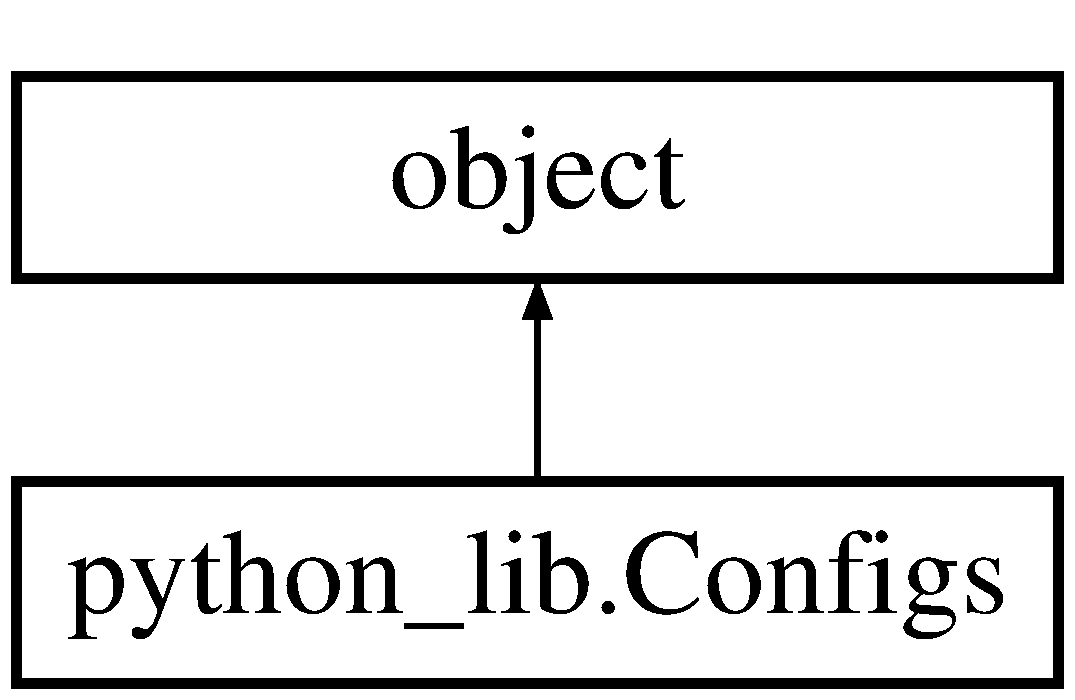
\includegraphics[height=2.000000cm]{classpython__lib_1_1_configs}
\end{center}
\end{figure}
\subsection*{Public Member Functions}
\begin{DoxyCompactItemize}
\item 
def \hyperlink{classpython__lib_1_1_configs_ab8338856ed3d266b0261606b75604612}{\-\_\-\-\_\-init\-\_\-\-\_\-}
\item 
def \hyperlink{classpython__lib_1_1_configs_acf2aa63cdb4635793ed21501743aacc1}{read\-\_\-config\-\_\-file}
\item 
def \hyperlink{classpython__lib_1_1_configs_a0afc89d68ccdd876e456ed21c0be25dc}{get}
\item 
def \hyperlink{classpython__lib_1_1_configs_a6488b0b6ce3fde518900de6d47b83f4f}{set}
\item 
def \hyperlink{classpython__lib_1_1_configs_a33404ffe7e17777f68576a126b0e5eb5}{show}
\item 
def \hyperlink{classpython__lib_1_1_configs_ad512301d0952867503d8d2ec8022c994}{show\-\_\-all}
\item 
def \hyperlink{classpython__lib_1_1_configs_a203b904533408187d81fe213aeb3545f}{reset\-\_\-action\-\_\-count}
\item 
def \hyperlink{classpython__lib_1_1_configs_a6061f898beac2fa1e700e36d76eef2f8}{reset}
\end{DoxyCompactItemize}


\subsection{Constructor \& Destructor Documentation}
\hypertarget{classpython__lib_1_1_configs_ab8338856ed3d266b0261606b75604612}{\index{python\-\_\-lib\-::\-Configs@{python\-\_\-lib\-::\-Configs}!\-\_\-\-\_\-init\-\_\-\-\_\-@{\-\_\-\-\_\-init\-\_\-\-\_\-}}
\index{\-\_\-\-\_\-init\-\_\-\-\_\-@{\-\_\-\-\_\-init\-\_\-\-\_\-}!python_lib::Configs@{python\-\_\-lib\-::\-Configs}}
\subsubsection[{\-\_\-\-\_\-init\-\_\-\-\_\-}]{\setlength{\rightskip}{0pt plus 5cm}def python\-\_\-lib.\-Configs.\-\_\-\-\_\-init\-\_\-\-\_\- (
\begin{DoxyParamCaption}
\item[{}]{self, }
\item[{}]{config\-\_\-file = {\ttfamily None}}
\end{DoxyParamCaption}
)}}\label{classpython__lib_1_1_configs_ab8338856ed3d266b0261606b75604612}


\subsection{Member Function Documentation}
\hypertarget{classpython__lib_1_1_configs_a0afc89d68ccdd876e456ed21c0be25dc}{\index{python\-\_\-lib\-::\-Configs@{python\-\_\-lib\-::\-Configs}!get@{get}}
\index{get@{get}!python_lib::Configs@{python\-\_\-lib\-::\-Configs}}
\subsubsection[{get}]{\setlength{\rightskip}{0pt plus 5cm}def python\-\_\-lib.\-Configs.\-get (
\begin{DoxyParamCaption}
\item[{}]{self, }
\item[{}]{key}
\end{DoxyParamCaption}
)}}\label{classpython__lib_1_1_configs_a0afc89d68ccdd876e456ed21c0be25dc}
\hypertarget{classpython__lib_1_1_configs_acf2aa63cdb4635793ed21501743aacc1}{\index{python\-\_\-lib\-::\-Configs@{python\-\_\-lib\-::\-Configs}!read\-\_\-config\-\_\-file@{read\-\_\-config\-\_\-file}}
\index{read\-\_\-config\-\_\-file@{read\-\_\-config\-\_\-file}!python_lib::Configs@{python\-\_\-lib\-::\-Configs}}
\subsubsection[{read\-\_\-config\-\_\-file}]{\setlength{\rightskip}{0pt plus 5cm}def python\-\_\-lib.\-Configs.\-read\-\_\-config\-\_\-file (
\begin{DoxyParamCaption}
\item[{}]{self, }
\item[{}]{config\-\_\-file}
\end{DoxyParamCaption}
)}}\label{classpython__lib_1_1_configs_acf2aa63cdb4635793ed21501743aacc1}
\hypertarget{classpython__lib_1_1_configs_a6061f898beac2fa1e700e36d76eef2f8}{\index{python\-\_\-lib\-::\-Configs@{python\-\_\-lib\-::\-Configs}!reset@{reset}}
\index{reset@{reset}!python_lib::Configs@{python\-\_\-lib\-::\-Configs}}
\subsubsection[{reset}]{\setlength{\rightskip}{0pt plus 5cm}def python\-\_\-lib.\-Configs.\-reset (
\begin{DoxyParamCaption}
\item[{}]{self}
\end{DoxyParamCaption}
)}}\label{classpython__lib_1_1_configs_a6061f898beac2fa1e700e36d76eef2f8}
\hypertarget{classpython__lib_1_1_configs_a203b904533408187d81fe213aeb3545f}{\index{python\-\_\-lib\-::\-Configs@{python\-\_\-lib\-::\-Configs}!reset\-\_\-action\-\_\-count@{reset\-\_\-action\-\_\-count}}
\index{reset\-\_\-action\-\_\-count@{reset\-\_\-action\-\_\-count}!python_lib::Configs@{python\-\_\-lib\-::\-Configs}}
\subsubsection[{reset\-\_\-action\-\_\-count}]{\setlength{\rightskip}{0pt plus 5cm}def python\-\_\-lib.\-Configs.\-reset\-\_\-action\-\_\-count (
\begin{DoxyParamCaption}
\item[{}]{self}
\end{DoxyParamCaption}
)}}\label{classpython__lib_1_1_configs_a203b904533408187d81fe213aeb3545f}
\hypertarget{classpython__lib_1_1_configs_a6488b0b6ce3fde518900de6d47b83f4f}{\index{python\-\_\-lib\-::\-Configs@{python\-\_\-lib\-::\-Configs}!set@{set}}
\index{set@{set}!python_lib::Configs@{python\-\_\-lib\-::\-Configs}}
\subsubsection[{set}]{\setlength{\rightskip}{0pt plus 5cm}def python\-\_\-lib.\-Configs.\-set (
\begin{DoxyParamCaption}
\item[{}]{self, }
\item[{}]{key, }
\item[{}]{value}
\end{DoxyParamCaption}
)}}\label{classpython__lib_1_1_configs_a6488b0b6ce3fde518900de6d47b83f4f}
\hypertarget{classpython__lib_1_1_configs_a33404ffe7e17777f68576a126b0e5eb5}{\index{python\-\_\-lib\-::\-Configs@{python\-\_\-lib\-::\-Configs}!show@{show}}
\index{show@{show}!python_lib::Configs@{python\-\_\-lib\-::\-Configs}}
\subsubsection[{show}]{\setlength{\rightskip}{0pt plus 5cm}def python\-\_\-lib.\-Configs.\-show (
\begin{DoxyParamCaption}
\item[{}]{self, }
\item[{}]{key}
\end{DoxyParamCaption}
)}}\label{classpython__lib_1_1_configs_a33404ffe7e17777f68576a126b0e5eb5}
\hypertarget{classpython__lib_1_1_configs_ad512301d0952867503d8d2ec8022c994}{\index{python\-\_\-lib\-::\-Configs@{python\-\_\-lib\-::\-Configs}!show\-\_\-all@{show\-\_\-all}}
\index{show\-\_\-all@{show\-\_\-all}!python_lib::Configs@{python\-\_\-lib\-::\-Configs}}
\subsubsection[{show\-\_\-all}]{\setlength{\rightskip}{0pt plus 5cm}def python\-\_\-lib.\-Configs.\-show\-\_\-all (
\begin{DoxyParamCaption}
\item[{}]{self}
\end{DoxyParamCaption}
)}}\label{classpython__lib_1_1_configs_ad512301d0952867503d8d2ec8022c994}


The documentation for this class was generated from the following file\-:\begin{DoxyCompactItemize}
\item 
\hyperlink{python__lib_8py}{python\-\_\-lib.\-py}\end{DoxyCompactItemize}

\hypertarget{classtcp__client_1_1_connections}{\section{tcp\-\_\-client.\-Connections Class Reference}
\label{classtcp__client_1_1_connections}\index{tcp\-\_\-client.\-Connections@{tcp\-\_\-client.\-Connections}}
}
Inheritance diagram for tcp\-\_\-client.\-Connections\-:\begin{figure}[H]
\begin{center}
\leavevmode
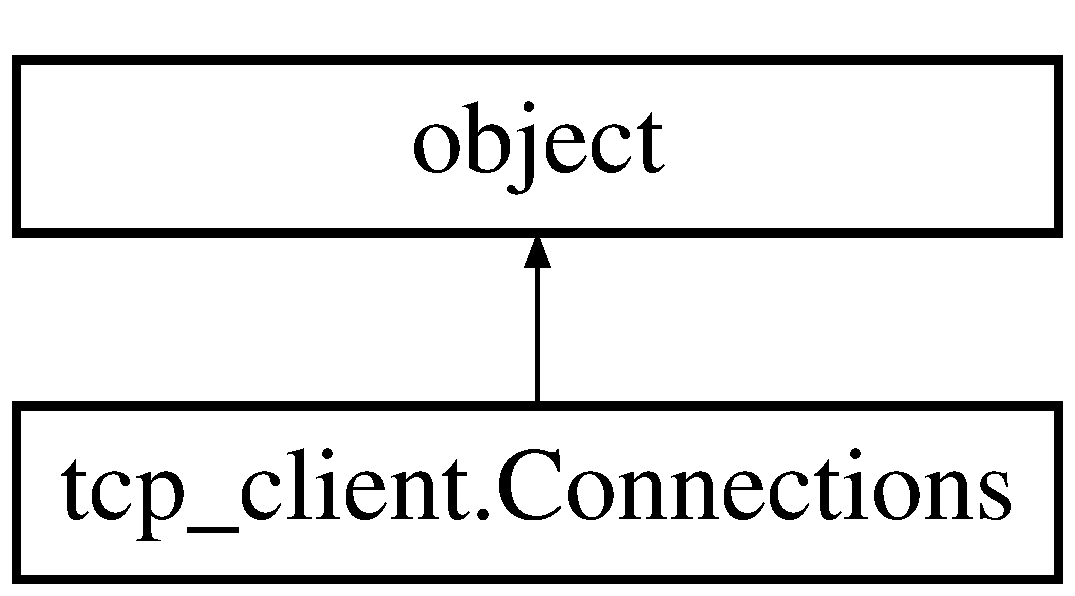
\includegraphics[height=2.000000cm]{classtcp__client_1_1_connections}
\end{center}
\end{figure}
\subsection*{Public Member Functions}
\begin{DoxyCompactItemize}
\item 
def \hyperlink{classtcp__client_1_1_connections_a4ee7df013d4db099277ccf24a4a46083}{\-\_\-\-\_\-init\-\_\-\-\_\-}
\item 
def \hyperlink{classtcp__client_1_1_connections_a826be86cbf939b2e25b2f54b33af27a2}{get\-\_\-sock}
\item 
def \hyperlink{classtcp__client_1_1_connections_ab5a93798eb1f7ae76da98b0236994840}{set\-\_\-sock}
\item 
def \hyperlink{classtcp__client_1_1_connections_af011521fe816f4747d025698e61cea68}{remove\-\_\-socket}
\end{DoxyCompactItemize}


\subsection{Detailed Description}
\begin{DoxyVerb}This class handles connections to servers.
\end{DoxyVerb}
 

\subsection{Constructor \& Destructor Documentation}
\hypertarget{classtcp__client_1_1_connections_a4ee7df013d4db099277ccf24a4a46083}{\index{tcp\-\_\-client\-::\-Connections@{tcp\-\_\-client\-::\-Connections}!\-\_\-\-\_\-init\-\_\-\-\_\-@{\-\_\-\-\_\-init\-\_\-\-\_\-}}
\index{\-\_\-\-\_\-init\-\_\-\-\_\-@{\-\_\-\-\_\-init\-\_\-\-\_\-}!tcp_client::Connections@{tcp\-\_\-client\-::\-Connections}}
\subsubsection[{\-\_\-\-\_\-init\-\_\-\-\_\-}]{\setlength{\rightskip}{0pt plus 5cm}def tcp\-\_\-client.\-Connections.\-\_\-\-\_\-init\-\_\-\-\_\- (
\begin{DoxyParamCaption}
\item[{}]{self}
\end{DoxyParamCaption}
)}}\label{classtcp__client_1_1_connections_a4ee7df013d4db099277ccf24a4a46083}


\subsection{Member Function Documentation}
\hypertarget{classtcp__client_1_1_connections_a826be86cbf939b2e25b2f54b33af27a2}{\index{tcp\-\_\-client\-::\-Connections@{tcp\-\_\-client\-::\-Connections}!get\-\_\-sock@{get\-\_\-sock}}
\index{get\-\_\-sock@{get\-\_\-sock}!tcp_client::Connections@{tcp\-\_\-client\-::\-Connections}}
\subsubsection[{get\-\_\-sock}]{\setlength{\rightskip}{0pt plus 5cm}def tcp\-\_\-client.\-Connections.\-get\-\_\-sock (
\begin{DoxyParamCaption}
\item[{}]{self, }
\item[{}]{c\-\_\-s\-\_\-pair}
\end{DoxyParamCaption}
)}}\label{classtcp__client_1_1_connections_a826be86cbf939b2e25b2f54b33af27a2}
\hypertarget{classtcp__client_1_1_connections_af011521fe816f4747d025698e61cea68}{\index{tcp\-\_\-client\-::\-Connections@{tcp\-\_\-client\-::\-Connections}!remove\-\_\-socket@{remove\-\_\-socket}}
\index{remove\-\_\-socket@{remove\-\_\-socket}!tcp_client::Connections@{tcp\-\_\-client\-::\-Connections}}
\subsubsection[{remove\-\_\-socket}]{\setlength{\rightskip}{0pt plus 5cm}def tcp\-\_\-client.\-Connections.\-remove\-\_\-socket (
\begin{DoxyParamCaption}
\item[{}]{self, }
\item[{}]{c\-\_\-s\-\_\-pair}
\end{DoxyParamCaption}
)}}\label{classtcp__client_1_1_connections_af011521fe816f4747d025698e61cea68}
\hypertarget{classtcp__client_1_1_connections_ab5a93798eb1f7ae76da98b0236994840}{\index{tcp\-\_\-client\-::\-Connections@{tcp\-\_\-client\-::\-Connections}!set\-\_\-sock@{set\-\_\-sock}}
\index{set\-\_\-sock@{set\-\_\-sock}!tcp_client::Connections@{tcp\-\_\-client\-::\-Connections}}
\subsubsection[{set\-\_\-sock}]{\setlength{\rightskip}{0pt plus 5cm}def tcp\-\_\-client.\-Connections.\-set\-\_\-sock (
\begin{DoxyParamCaption}
\item[{}]{self, }
\item[{}]{c\-\_\-s\-\_\-pair, }
\item[{}]{socket}
\end{DoxyParamCaption}
)}}\label{classtcp__client_1_1_connections_ab5a93798eb1f7ae76da98b0236994840}


The documentation for this class was generated from the following file\-:\begin{DoxyCompactItemize}
\item 
\hyperlink{tcp__client_8py}{tcp\-\_\-client.\-py}\end{DoxyCompactItemize}

\hypertarget{classcdf_1_1_data_point}{\section{cdf.\-Data\-Point Class Reference}
\label{classcdf_1_1_data_point}\index{cdf.\-Data\-Point@{cdf.\-Data\-Point}}
}
Inheritance diagram for cdf.\-Data\-Point\-:\begin{figure}[H]
\begin{center}
\leavevmode
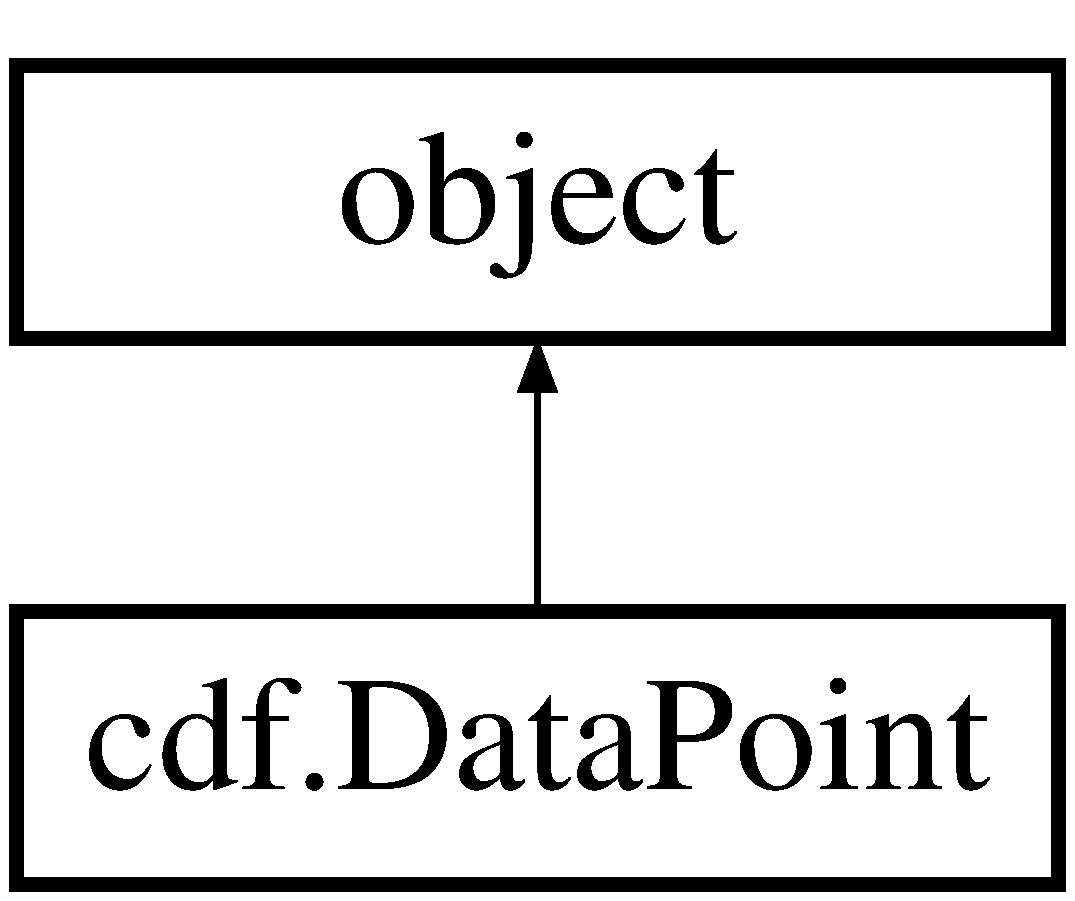
\includegraphics[height=2.000000cm]{classcdf_1_1_data_point}
\end{center}
\end{figure}
\subsection*{Public Member Functions}
\begin{DoxyCompactItemize}
\item 
def \hyperlink{classcdf_1_1_data_point_a99f0e404b101fd170b6b3a05478d43a1}{\-\_\-\-\_\-init\-\_\-\-\_\-}
\item 
def \hyperlink{classcdf_1_1_data_point_a9115a84a0ed18a7f79e18b63928e72ce}{show}
\end{DoxyCompactItemize}
\subsection*{Public Attributes}
\begin{DoxyCompactItemize}
\item 
\hyperlink{classcdf_1_1_data_point_ad73a5f02299af4166f516ebcf70aa2be}{begin}
\item 
\hyperlink{classcdf_1_1_data_point_a02ee1a6a3e1cad6aaca067751c30952c}{end}
\item 
\hyperlink{classcdf_1_1_data_point_a52817194109fae73a5cc2d7595797a65}{frames}
\item 
\hyperlink{classcdf_1_1_data_point_aa098d368a57503bfc327e76f34d211e4}{bytes}
\item 
\hyperlink{classcdf_1_1_data_point_adc4cd93ff514639bc9bb75301433567a}{xput}
\end{DoxyCompactItemize}


\subsection{Constructor \& Destructor Documentation}
\hypertarget{classcdf_1_1_data_point_a99f0e404b101fd170b6b3a05478d43a1}{\index{cdf\-::\-Data\-Point@{cdf\-::\-Data\-Point}!\-\_\-\-\_\-init\-\_\-\-\_\-@{\-\_\-\-\_\-init\-\_\-\-\_\-}}
\index{\-\_\-\-\_\-init\-\_\-\-\_\-@{\-\_\-\-\_\-init\-\_\-\-\_\-}!cdf::DataPoint@{cdf\-::\-Data\-Point}}
\subsubsection[{\-\_\-\-\_\-init\-\_\-\-\_\-}]{\setlength{\rightskip}{0pt plus 5cm}def cdf.\-Data\-Point.\-\_\-\-\_\-init\-\_\-\-\_\- (
\begin{DoxyParamCaption}
\item[{}]{self, }
\item[{}]{begin, }
\item[{}]{end, }
\item[{}]{frames, }
\item[{}]{bytes}
\end{DoxyParamCaption}
)}}\label{classcdf_1_1_data_point_a99f0e404b101fd170b6b3a05478d43a1}


\subsection{Member Function Documentation}
\hypertarget{classcdf_1_1_data_point_a9115a84a0ed18a7f79e18b63928e72ce}{\index{cdf\-::\-Data\-Point@{cdf\-::\-Data\-Point}!show@{show}}
\index{show@{show}!cdf::DataPoint@{cdf\-::\-Data\-Point}}
\subsubsection[{show}]{\setlength{\rightskip}{0pt plus 5cm}def cdf.\-Data\-Point.\-show (
\begin{DoxyParamCaption}
\item[{}]{self}
\end{DoxyParamCaption}
)}}\label{classcdf_1_1_data_point_a9115a84a0ed18a7f79e18b63928e72ce}


\subsection{Member Data Documentation}
\hypertarget{classcdf_1_1_data_point_ad73a5f02299af4166f516ebcf70aa2be}{\index{cdf\-::\-Data\-Point@{cdf\-::\-Data\-Point}!begin@{begin}}
\index{begin@{begin}!cdf::DataPoint@{cdf\-::\-Data\-Point}}
\subsubsection[{begin}]{\setlength{\rightskip}{0pt plus 5cm}cdf.\-Data\-Point.\-begin}}\label{classcdf_1_1_data_point_ad73a5f02299af4166f516ebcf70aa2be}
\hypertarget{classcdf_1_1_data_point_aa098d368a57503bfc327e76f34d211e4}{\index{cdf\-::\-Data\-Point@{cdf\-::\-Data\-Point}!bytes@{bytes}}
\index{bytes@{bytes}!cdf::DataPoint@{cdf\-::\-Data\-Point}}
\subsubsection[{bytes}]{\setlength{\rightskip}{0pt plus 5cm}cdf.\-Data\-Point.\-bytes}}\label{classcdf_1_1_data_point_aa098d368a57503bfc327e76f34d211e4}
\hypertarget{classcdf_1_1_data_point_a02ee1a6a3e1cad6aaca067751c30952c}{\index{cdf\-::\-Data\-Point@{cdf\-::\-Data\-Point}!end@{end}}
\index{end@{end}!cdf::DataPoint@{cdf\-::\-Data\-Point}}
\subsubsection[{end}]{\setlength{\rightskip}{0pt plus 5cm}cdf.\-Data\-Point.\-end}}\label{classcdf_1_1_data_point_a02ee1a6a3e1cad6aaca067751c30952c}
\hypertarget{classcdf_1_1_data_point_a52817194109fae73a5cc2d7595797a65}{\index{cdf\-::\-Data\-Point@{cdf\-::\-Data\-Point}!frames@{frames}}
\index{frames@{frames}!cdf::DataPoint@{cdf\-::\-Data\-Point}}
\subsubsection[{frames}]{\setlength{\rightskip}{0pt plus 5cm}cdf.\-Data\-Point.\-frames}}\label{classcdf_1_1_data_point_a52817194109fae73a5cc2d7595797a65}
\hypertarget{classcdf_1_1_data_point_adc4cd93ff514639bc9bb75301433567a}{\index{cdf\-::\-Data\-Point@{cdf\-::\-Data\-Point}!xput@{xput}}
\index{xput@{xput}!cdf::DataPoint@{cdf\-::\-Data\-Point}}
\subsubsection[{xput}]{\setlength{\rightskip}{0pt plus 5cm}cdf.\-Data\-Point.\-xput}}\label{classcdf_1_1_data_point_adc4cd93ff514639bc9bb75301433567a}


The documentation for this class was generated from the following file\-:\begin{DoxyCompactItemize}
\item 
\hyperlink{cdf_8py}{cdf.\-py}\end{DoxyCompactItemize}

\hypertarget{classks2_1_1_data_point}{\section{ks2.\-Data\-Point Class Reference}
\label{classks2_1_1_data_point}\index{ks2.\-Data\-Point@{ks2.\-Data\-Point}}
}
Inheritance diagram for ks2.\-Data\-Point\-:\begin{figure}[H]
\begin{center}
\leavevmode
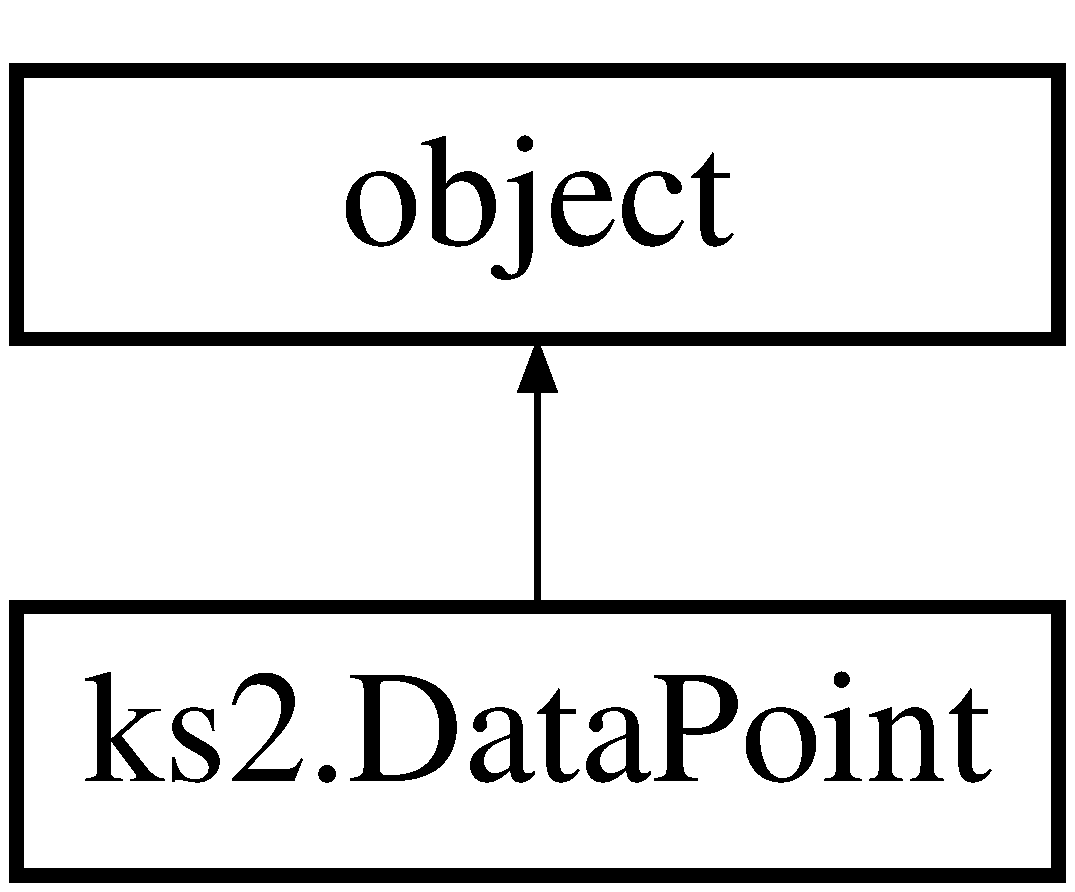
\includegraphics[height=2.000000cm]{classks2_1_1_data_point}
\end{center}
\end{figure}
\subsection*{Public Member Functions}
\begin{DoxyCompactItemize}
\item 
def \hyperlink{classks2_1_1_data_point_ab22340cdf5d06004c1c96c75c5ee0138}{\-\_\-\-\_\-init\-\_\-\-\_\-}
\item 
def \hyperlink{classks2_1_1_data_point_a828583eba2493fdcd5d05a1dc34be764}{show}
\end{DoxyCompactItemize}
\subsection*{Public Attributes}
\begin{DoxyCompactItemize}
\item 
\hyperlink{classks2_1_1_data_point_a5109060f0ce2171d154560ae1f7ea618}{begin}
\item 
\hyperlink{classks2_1_1_data_point_a4898a56ed7246eb33a295da6496566d6}{end}
\item 
\hyperlink{classks2_1_1_data_point_a214dead1966be1f38aa5bb5858ba8bf6}{frames}
\item 
\hyperlink{classks2_1_1_data_point_ad5e6469cea32af6efb8803f300bb9dee}{bytes}
\item 
\hyperlink{classks2_1_1_data_point_a129a9557c8d54633b893753d8e272423}{xput}
\end{DoxyCompactItemize}


\subsection{Constructor \& Destructor Documentation}
\hypertarget{classks2_1_1_data_point_ab22340cdf5d06004c1c96c75c5ee0138}{\index{ks2\-::\-Data\-Point@{ks2\-::\-Data\-Point}!\-\_\-\-\_\-init\-\_\-\-\_\-@{\-\_\-\-\_\-init\-\_\-\-\_\-}}
\index{\-\_\-\-\_\-init\-\_\-\-\_\-@{\-\_\-\-\_\-init\-\_\-\-\_\-}!ks2::DataPoint@{ks2\-::\-Data\-Point}}
\subsubsection[{\-\_\-\-\_\-init\-\_\-\-\_\-}]{\setlength{\rightskip}{0pt plus 5cm}def ks2.\-Data\-Point.\-\_\-\-\_\-init\-\_\-\-\_\- (
\begin{DoxyParamCaption}
\item[{}]{self, }
\item[{}]{begin, }
\item[{}]{end, }
\item[{}]{frames, }
\item[{}]{bytes}
\end{DoxyParamCaption}
)}}\label{classks2_1_1_data_point_ab22340cdf5d06004c1c96c75c5ee0138}


\subsection{Member Function Documentation}
\hypertarget{classks2_1_1_data_point_a828583eba2493fdcd5d05a1dc34be764}{\index{ks2\-::\-Data\-Point@{ks2\-::\-Data\-Point}!show@{show}}
\index{show@{show}!ks2::DataPoint@{ks2\-::\-Data\-Point}}
\subsubsection[{show}]{\setlength{\rightskip}{0pt plus 5cm}def ks2.\-Data\-Point.\-show (
\begin{DoxyParamCaption}
\item[{}]{self}
\end{DoxyParamCaption}
)}}\label{classks2_1_1_data_point_a828583eba2493fdcd5d05a1dc34be764}


\subsection{Member Data Documentation}
\hypertarget{classks2_1_1_data_point_a5109060f0ce2171d154560ae1f7ea618}{\index{ks2\-::\-Data\-Point@{ks2\-::\-Data\-Point}!begin@{begin}}
\index{begin@{begin}!ks2::DataPoint@{ks2\-::\-Data\-Point}}
\subsubsection[{begin}]{\setlength{\rightskip}{0pt plus 5cm}ks2.\-Data\-Point.\-begin}}\label{classks2_1_1_data_point_a5109060f0ce2171d154560ae1f7ea618}
\hypertarget{classks2_1_1_data_point_ad5e6469cea32af6efb8803f300bb9dee}{\index{ks2\-::\-Data\-Point@{ks2\-::\-Data\-Point}!bytes@{bytes}}
\index{bytes@{bytes}!ks2::DataPoint@{ks2\-::\-Data\-Point}}
\subsubsection[{bytes}]{\setlength{\rightskip}{0pt plus 5cm}ks2.\-Data\-Point.\-bytes}}\label{classks2_1_1_data_point_ad5e6469cea32af6efb8803f300bb9dee}
\hypertarget{classks2_1_1_data_point_a4898a56ed7246eb33a295da6496566d6}{\index{ks2\-::\-Data\-Point@{ks2\-::\-Data\-Point}!end@{end}}
\index{end@{end}!ks2::DataPoint@{ks2\-::\-Data\-Point}}
\subsubsection[{end}]{\setlength{\rightskip}{0pt plus 5cm}ks2.\-Data\-Point.\-end}}\label{classks2_1_1_data_point_a4898a56ed7246eb33a295da6496566d6}
\hypertarget{classks2_1_1_data_point_a214dead1966be1f38aa5bb5858ba8bf6}{\index{ks2\-::\-Data\-Point@{ks2\-::\-Data\-Point}!frames@{frames}}
\index{frames@{frames}!ks2::DataPoint@{ks2\-::\-Data\-Point}}
\subsubsection[{frames}]{\setlength{\rightskip}{0pt plus 5cm}ks2.\-Data\-Point.\-frames}}\label{classks2_1_1_data_point_a214dead1966be1f38aa5bb5858ba8bf6}
\hypertarget{classks2_1_1_data_point_a129a9557c8d54633b893753d8e272423}{\index{ks2\-::\-Data\-Point@{ks2\-::\-Data\-Point}!xput@{xput}}
\index{xput@{xput}!ks2::DataPoint@{ks2\-::\-Data\-Point}}
\subsubsection[{xput}]{\setlength{\rightskip}{0pt plus 5cm}ks2.\-Data\-Point.\-xput}}\label{classks2_1_1_data_point_a129a9557c8d54633b893753d8e272423}


The documentation for this class was generated from the following file\-:\begin{DoxyCompactItemize}
\item 
\hyperlink{ks2_8py}{ks2.\-py}\end{DoxyCompactItemize}

\hypertarget{classthrouput__tshark_1_1_data_point}{\section{throuput\-\_\-tshark.\-Data\-Point Class Reference}
\label{classthrouput__tshark_1_1_data_point}\index{throuput\-\_\-tshark.\-Data\-Point@{throuput\-\_\-tshark.\-Data\-Point}}
}
Inheritance diagram for throuput\-\_\-tshark.\-Data\-Point\-:\begin{figure}[H]
\begin{center}
\leavevmode
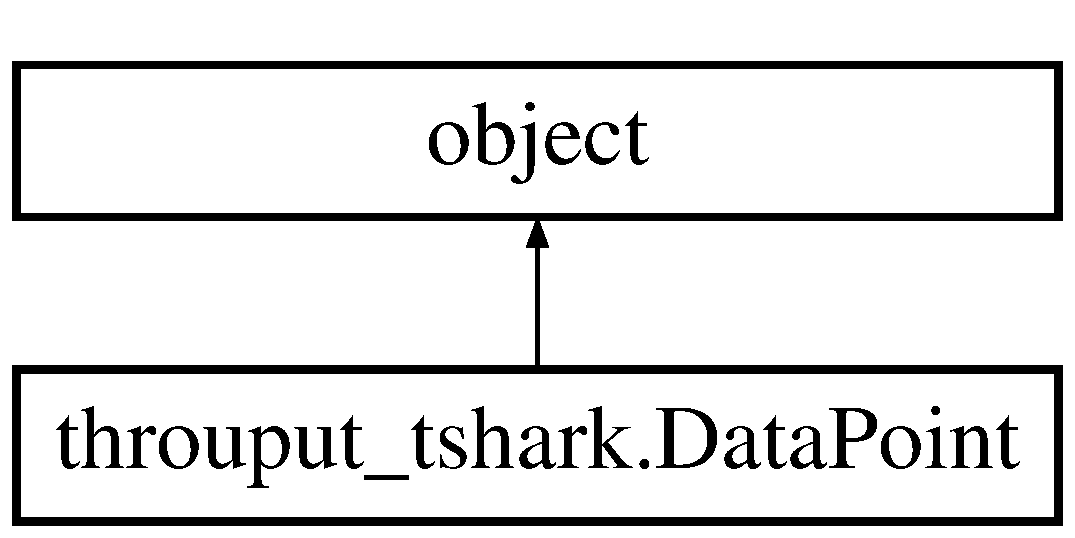
\includegraphics[height=2.000000cm]{classthrouput__tshark_1_1_data_point}
\end{center}
\end{figure}
\subsection*{Public Member Functions}
\begin{DoxyCompactItemize}
\item 
def \hyperlink{classthrouput__tshark_1_1_data_point_a47914d6bfeb17b2bf09b7332e6f7ea0e}{\-\_\-\-\_\-init\-\_\-\-\_\-}
\item 
def \hyperlink{classthrouput__tshark_1_1_data_point_abb42b35551c9bfa4a11348d9bf972591}{show}
\end{DoxyCompactItemize}
\subsection*{Public Attributes}
\begin{DoxyCompactItemize}
\item 
\hyperlink{classthrouput__tshark_1_1_data_point_a40bc440085947ec24669e6e5f6c5ddb8}{begin}
\item 
\hyperlink{classthrouput__tshark_1_1_data_point_a04d37b8f30e79e4b8caa963cafb5dd70}{end}
\item 
\hyperlink{classthrouput__tshark_1_1_data_point_a54eab4264d03efb8ec893e85259954c3}{frames}
\item 
\hyperlink{classthrouput__tshark_1_1_data_point_aa9801c08e336468d076ff21e43c817c8}{bytes}
\item 
\hyperlink{classthrouput__tshark_1_1_data_point_aca3722436083ff0c4f619bf32ae2e893}{xput}
\end{DoxyCompactItemize}


\subsection{Constructor \& Destructor Documentation}
\hypertarget{classthrouput__tshark_1_1_data_point_a47914d6bfeb17b2bf09b7332e6f7ea0e}{\index{throuput\-\_\-tshark\-::\-Data\-Point@{throuput\-\_\-tshark\-::\-Data\-Point}!\-\_\-\-\_\-init\-\_\-\-\_\-@{\-\_\-\-\_\-init\-\_\-\-\_\-}}
\index{\-\_\-\-\_\-init\-\_\-\-\_\-@{\-\_\-\-\_\-init\-\_\-\-\_\-}!throuput_tshark::DataPoint@{throuput\-\_\-tshark\-::\-Data\-Point}}
\subsubsection[{\-\_\-\-\_\-init\-\_\-\-\_\-}]{\setlength{\rightskip}{0pt plus 5cm}def throuput\-\_\-tshark.\-Data\-Point.\-\_\-\-\_\-init\-\_\-\-\_\- (
\begin{DoxyParamCaption}
\item[{}]{self, }
\item[{}]{begin, }
\item[{}]{end, }
\item[{}]{frames, }
\item[{}]{bytes}
\end{DoxyParamCaption}
)}}\label{classthrouput__tshark_1_1_data_point_a47914d6bfeb17b2bf09b7332e6f7ea0e}


\subsection{Member Function Documentation}
\hypertarget{classthrouput__tshark_1_1_data_point_abb42b35551c9bfa4a11348d9bf972591}{\index{throuput\-\_\-tshark\-::\-Data\-Point@{throuput\-\_\-tshark\-::\-Data\-Point}!show@{show}}
\index{show@{show}!throuput_tshark::DataPoint@{throuput\-\_\-tshark\-::\-Data\-Point}}
\subsubsection[{show}]{\setlength{\rightskip}{0pt plus 5cm}def throuput\-\_\-tshark.\-Data\-Point.\-show (
\begin{DoxyParamCaption}
\item[{}]{self}
\end{DoxyParamCaption}
)}}\label{classthrouput__tshark_1_1_data_point_abb42b35551c9bfa4a11348d9bf972591}


\subsection{Member Data Documentation}
\hypertarget{classthrouput__tshark_1_1_data_point_a40bc440085947ec24669e6e5f6c5ddb8}{\index{throuput\-\_\-tshark\-::\-Data\-Point@{throuput\-\_\-tshark\-::\-Data\-Point}!begin@{begin}}
\index{begin@{begin}!throuput_tshark::DataPoint@{throuput\-\_\-tshark\-::\-Data\-Point}}
\subsubsection[{begin}]{\setlength{\rightskip}{0pt plus 5cm}throuput\-\_\-tshark.\-Data\-Point.\-begin}}\label{classthrouput__tshark_1_1_data_point_a40bc440085947ec24669e6e5f6c5ddb8}
\hypertarget{classthrouput__tshark_1_1_data_point_aa9801c08e336468d076ff21e43c817c8}{\index{throuput\-\_\-tshark\-::\-Data\-Point@{throuput\-\_\-tshark\-::\-Data\-Point}!bytes@{bytes}}
\index{bytes@{bytes}!throuput_tshark::DataPoint@{throuput\-\_\-tshark\-::\-Data\-Point}}
\subsubsection[{bytes}]{\setlength{\rightskip}{0pt plus 5cm}throuput\-\_\-tshark.\-Data\-Point.\-bytes}}\label{classthrouput__tshark_1_1_data_point_aa9801c08e336468d076ff21e43c817c8}
\hypertarget{classthrouput__tshark_1_1_data_point_a04d37b8f30e79e4b8caa963cafb5dd70}{\index{throuput\-\_\-tshark\-::\-Data\-Point@{throuput\-\_\-tshark\-::\-Data\-Point}!end@{end}}
\index{end@{end}!throuput_tshark::DataPoint@{throuput\-\_\-tshark\-::\-Data\-Point}}
\subsubsection[{end}]{\setlength{\rightskip}{0pt plus 5cm}throuput\-\_\-tshark.\-Data\-Point.\-end}}\label{classthrouput__tshark_1_1_data_point_a04d37b8f30e79e4b8caa963cafb5dd70}
\hypertarget{classthrouput__tshark_1_1_data_point_a54eab4264d03efb8ec893e85259954c3}{\index{throuput\-\_\-tshark\-::\-Data\-Point@{throuput\-\_\-tshark\-::\-Data\-Point}!frames@{frames}}
\index{frames@{frames}!throuput_tshark::DataPoint@{throuput\-\_\-tshark\-::\-Data\-Point}}
\subsubsection[{frames}]{\setlength{\rightskip}{0pt plus 5cm}throuput\-\_\-tshark.\-Data\-Point.\-frames}}\label{classthrouput__tshark_1_1_data_point_a54eab4264d03efb8ec893e85259954c3}
\hypertarget{classthrouput__tshark_1_1_data_point_aca3722436083ff0c4f619bf32ae2e893}{\index{throuput\-\_\-tshark\-::\-Data\-Point@{throuput\-\_\-tshark\-::\-Data\-Point}!xput@{xput}}
\index{xput@{xput}!throuput_tshark::DataPoint@{throuput\-\_\-tshark\-::\-Data\-Point}}
\subsubsection[{xput}]{\setlength{\rightskip}{0pt plus 5cm}throuput\-\_\-tshark.\-Data\-Point.\-xput}}\label{classthrouput__tshark_1_1_data_point_aca3722436083ff0c4f619bf32ae2e893}


The documentation for this class was generated from the following file\-:\begin{DoxyCompactItemize}
\item 
\hyperlink{throuput__tshark_8py}{throuput\-\_\-tshark.\-py}\end{DoxyCompactItemize}

\hypertarget{classcdf_1_1_dump_stat}{\section{cdf.\-Dump\-Stat Class Reference}
\label{classcdf_1_1_dump_stat}\index{cdf.\-Dump\-Stat@{cdf.\-Dump\-Stat}}
}
Inheritance diagram for cdf.\-Dump\-Stat\-:\begin{figure}[H]
\begin{center}
\leavevmode
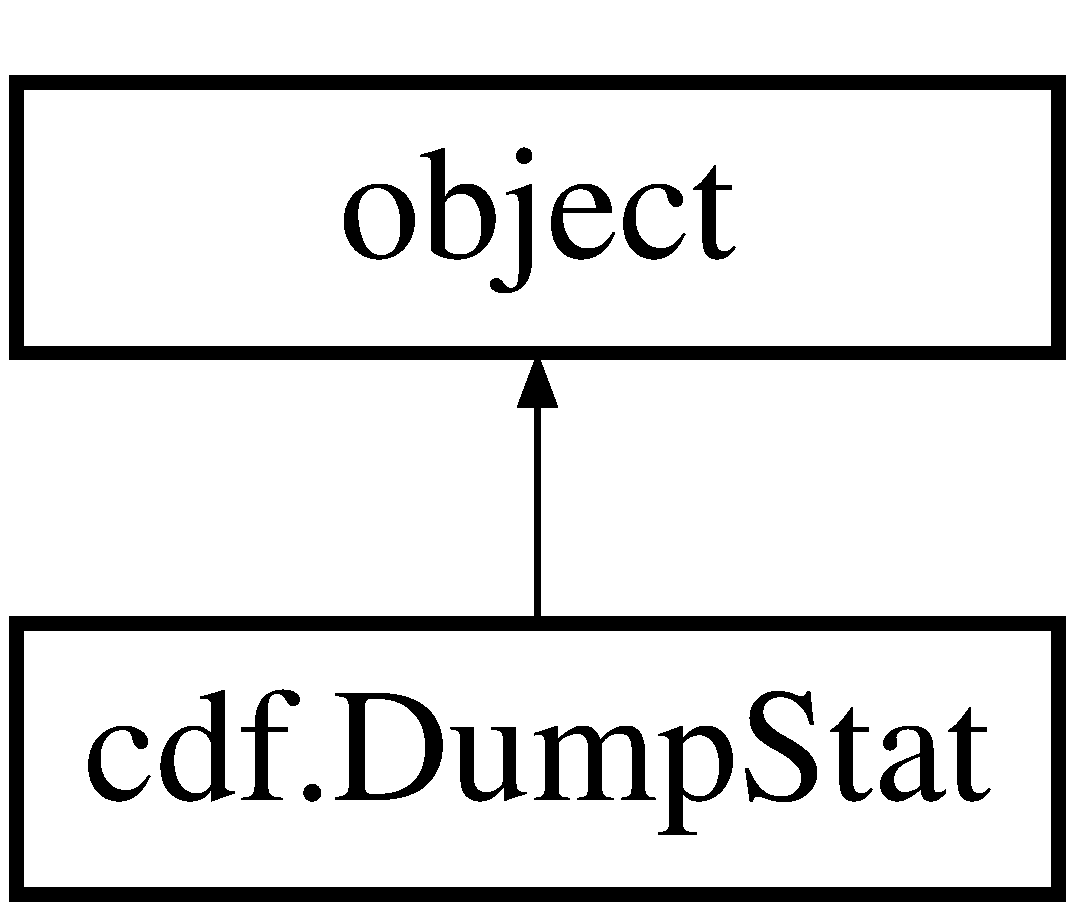
\includegraphics[height=2.000000cm]{classcdf_1_1_dump_stat}
\end{center}
\end{figure}
\subsection*{Public Member Functions}
\begin{DoxyCompactItemize}
\item 
def \hyperlink{classcdf_1_1_dump_stat_a5eec4a8104f13d0db2f52550939c063b}{\-\_\-\-\_\-init\-\_\-\-\_\-}
\item 
def \hyperlink{classcdf_1_1_dump_stat_a87ad3364e5d578a2939d0320d3befbd6}{show}
\item 
def \hyperlink{classcdf_1_1_dump_stat_a0c1bee4cb7e81c95688fd4aaa27f7373}{two\-\_\-decimal}
\end{DoxyCompactItemize}
\subsection*{Public Attributes}
\begin{DoxyCompactItemize}
\item 
\hyperlink{classcdf_1_1_dump_stat_ae693ca73d82126845880b10f07a82d94}{name}
\item 
\hyperlink{classcdf_1_1_dump_stat_acdcf65c5f0eedeb9c559099b6e817ea8}{xput\-\_\-min}
\item 
\hyperlink{classcdf_1_1_dump_stat_a2b3385cc8e90523350f8c8f280f8d2ae}{xput\-\_\-max}
\item 
\hyperlink{classcdf_1_1_dump_stat_a098a66c8979c1be0a7754ef568337a5b}{xput\-\_\-median}
\item 
\hyperlink{classcdf_1_1_dump_stat_a9a78dcffdce2a4a6164703e2efb6c519}{xput\-\_\-avg}
\item 
\hyperlink{classcdf_1_1_dump_stat_a2736270ac68b05550848435b6a291b3e}{xput\-\_\-std}
\end{DoxyCompactItemize}


\subsection{Constructor \& Destructor Documentation}
\hypertarget{classcdf_1_1_dump_stat_a5eec4a8104f13d0db2f52550939c063b}{\index{cdf\-::\-Dump\-Stat@{cdf\-::\-Dump\-Stat}!\-\_\-\-\_\-init\-\_\-\-\_\-@{\-\_\-\-\_\-init\-\_\-\-\_\-}}
\index{\-\_\-\-\_\-init\-\_\-\-\_\-@{\-\_\-\-\_\-init\-\_\-\-\_\-}!cdf::DumpStat@{cdf\-::\-Dump\-Stat}}
\subsubsection[{\-\_\-\-\_\-init\-\_\-\-\_\-}]{\setlength{\rightskip}{0pt plus 5cm}def cdf.\-Dump\-Stat.\-\_\-\-\_\-init\-\_\-\-\_\- (
\begin{DoxyParamCaption}
\item[{}]{self, }
\item[{}]{xput\-\_\-min, }
\item[{}]{xput\-\_\-max, }
\item[{}]{xput\-\_\-median, }
\item[{}]{xput\-\_\-avg, }
\item[{}]{xput\-\_\-std, }
\item[{}]{name = {\ttfamily None}}
\end{DoxyParamCaption}
)}}\label{classcdf_1_1_dump_stat_a5eec4a8104f13d0db2f52550939c063b}


\subsection{Member Function Documentation}
\hypertarget{classcdf_1_1_dump_stat_a87ad3364e5d578a2939d0320d3befbd6}{\index{cdf\-::\-Dump\-Stat@{cdf\-::\-Dump\-Stat}!show@{show}}
\index{show@{show}!cdf::DumpStat@{cdf\-::\-Dump\-Stat}}
\subsubsection[{show}]{\setlength{\rightskip}{0pt plus 5cm}def cdf.\-Dump\-Stat.\-show (
\begin{DoxyParamCaption}
\item[{}]{self, }
\item[{}]{row = {\ttfamily False}}
\end{DoxyParamCaption}
)}}\label{classcdf_1_1_dump_stat_a87ad3364e5d578a2939d0320d3befbd6}
\hypertarget{classcdf_1_1_dump_stat_a0c1bee4cb7e81c95688fd4aaa27f7373}{\index{cdf\-::\-Dump\-Stat@{cdf\-::\-Dump\-Stat}!two\-\_\-decimal@{two\-\_\-decimal}}
\index{two\-\_\-decimal@{two\-\_\-decimal}!cdf::DumpStat@{cdf\-::\-Dump\-Stat}}
\subsubsection[{two\-\_\-decimal}]{\setlength{\rightskip}{0pt plus 5cm}def cdf.\-Dump\-Stat.\-two\-\_\-decimal (
\begin{DoxyParamCaption}
\item[{}]{self}
\end{DoxyParamCaption}
)}}\label{classcdf_1_1_dump_stat_a0c1bee4cb7e81c95688fd4aaa27f7373}


\subsection{Member Data Documentation}
\hypertarget{classcdf_1_1_dump_stat_ae693ca73d82126845880b10f07a82d94}{\index{cdf\-::\-Dump\-Stat@{cdf\-::\-Dump\-Stat}!name@{name}}
\index{name@{name}!cdf::DumpStat@{cdf\-::\-Dump\-Stat}}
\subsubsection[{name}]{\setlength{\rightskip}{0pt plus 5cm}cdf.\-Dump\-Stat.\-name}}\label{classcdf_1_1_dump_stat_ae693ca73d82126845880b10f07a82d94}
\hypertarget{classcdf_1_1_dump_stat_a9a78dcffdce2a4a6164703e2efb6c519}{\index{cdf\-::\-Dump\-Stat@{cdf\-::\-Dump\-Stat}!xput\-\_\-avg@{xput\-\_\-avg}}
\index{xput\-\_\-avg@{xput\-\_\-avg}!cdf::DumpStat@{cdf\-::\-Dump\-Stat}}
\subsubsection[{xput\-\_\-avg}]{\setlength{\rightskip}{0pt plus 5cm}cdf.\-Dump\-Stat.\-xput\-\_\-avg}}\label{classcdf_1_1_dump_stat_a9a78dcffdce2a4a6164703e2efb6c519}
\hypertarget{classcdf_1_1_dump_stat_a2b3385cc8e90523350f8c8f280f8d2ae}{\index{cdf\-::\-Dump\-Stat@{cdf\-::\-Dump\-Stat}!xput\-\_\-max@{xput\-\_\-max}}
\index{xput\-\_\-max@{xput\-\_\-max}!cdf::DumpStat@{cdf\-::\-Dump\-Stat}}
\subsubsection[{xput\-\_\-max}]{\setlength{\rightskip}{0pt plus 5cm}cdf.\-Dump\-Stat.\-xput\-\_\-max}}\label{classcdf_1_1_dump_stat_a2b3385cc8e90523350f8c8f280f8d2ae}
\hypertarget{classcdf_1_1_dump_stat_a098a66c8979c1be0a7754ef568337a5b}{\index{cdf\-::\-Dump\-Stat@{cdf\-::\-Dump\-Stat}!xput\-\_\-median@{xput\-\_\-median}}
\index{xput\-\_\-median@{xput\-\_\-median}!cdf::DumpStat@{cdf\-::\-Dump\-Stat}}
\subsubsection[{xput\-\_\-median}]{\setlength{\rightskip}{0pt plus 5cm}cdf.\-Dump\-Stat.\-xput\-\_\-median}}\label{classcdf_1_1_dump_stat_a098a66c8979c1be0a7754ef568337a5b}
\hypertarget{classcdf_1_1_dump_stat_acdcf65c5f0eedeb9c559099b6e817ea8}{\index{cdf\-::\-Dump\-Stat@{cdf\-::\-Dump\-Stat}!xput\-\_\-min@{xput\-\_\-min}}
\index{xput\-\_\-min@{xput\-\_\-min}!cdf::DumpStat@{cdf\-::\-Dump\-Stat}}
\subsubsection[{xput\-\_\-min}]{\setlength{\rightskip}{0pt plus 5cm}cdf.\-Dump\-Stat.\-xput\-\_\-min}}\label{classcdf_1_1_dump_stat_acdcf65c5f0eedeb9c559099b6e817ea8}
\hypertarget{classcdf_1_1_dump_stat_a2736270ac68b05550848435b6a291b3e}{\index{cdf\-::\-Dump\-Stat@{cdf\-::\-Dump\-Stat}!xput\-\_\-std@{xput\-\_\-std}}
\index{xput\-\_\-std@{xput\-\_\-std}!cdf::DumpStat@{cdf\-::\-Dump\-Stat}}
\subsubsection[{xput\-\_\-std}]{\setlength{\rightskip}{0pt plus 5cm}cdf.\-Dump\-Stat.\-xput\-\_\-std}}\label{classcdf_1_1_dump_stat_a2736270ac68b05550848435b6a291b3e}


The documentation for this class was generated from the following file\-:\begin{DoxyCompactItemize}
\item 
\hyperlink{cdf_8py}{cdf.\-py}\end{DoxyCompactItemize}

\hypertarget{classthrouput__tshark_1_1_dump_stat}{\section{throuput\-\_\-tshark.\-Dump\-Stat Class Reference}
\label{classthrouput__tshark_1_1_dump_stat}\index{throuput\-\_\-tshark.\-Dump\-Stat@{throuput\-\_\-tshark.\-Dump\-Stat}}
}
Inheritance diagram for throuput\-\_\-tshark.\-Dump\-Stat\-:\begin{figure}[H]
\begin{center}
\leavevmode
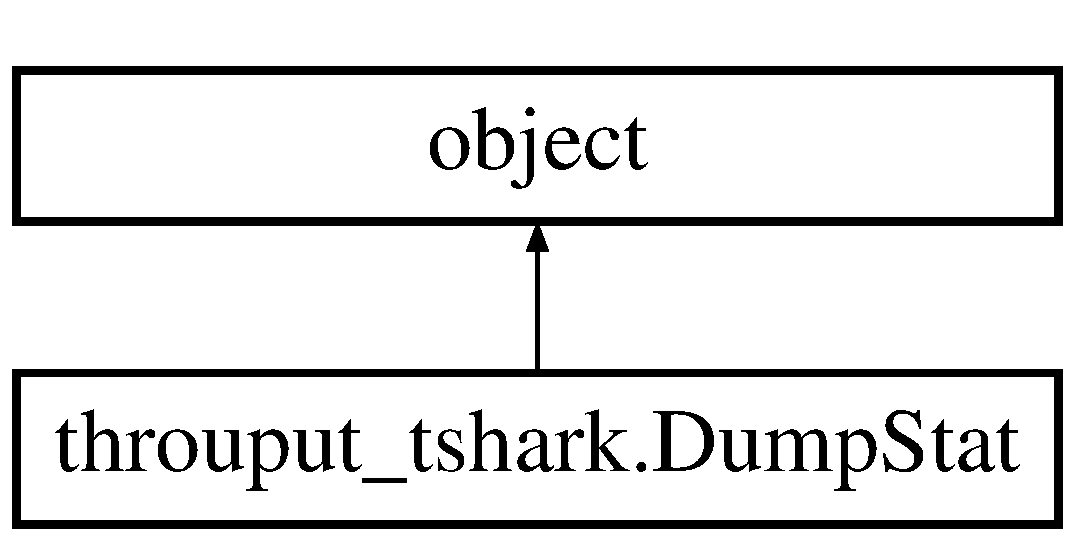
\includegraphics[height=2.000000cm]{classthrouput__tshark_1_1_dump_stat}
\end{center}
\end{figure}
\subsection*{Public Member Functions}
\begin{DoxyCompactItemize}
\item 
def \hyperlink{classthrouput__tshark_1_1_dump_stat_a0d29689f383bac8dd525a3ed23c74d00}{\-\_\-\-\_\-init\-\_\-\-\_\-}
\item 
def \hyperlink{classthrouput__tshark_1_1_dump_stat_ac45218a7a6a5441f2c4df7271762697a}{show}
\item 
def \hyperlink{classthrouput__tshark_1_1_dump_stat_a6641d527896c116977d19a27e84db04e}{two\-\_\-decimal}
\end{DoxyCompactItemize}
\subsection*{Public Attributes}
\begin{DoxyCompactItemize}
\item 
\hyperlink{classthrouput__tshark_1_1_dump_stat_a1c4c3a2c6b7d0567fafafc8ed99b9234}{name}
\item 
\hyperlink{classthrouput__tshark_1_1_dump_stat_a353c7d18a6ab1cf675fe48414db842f6}{xput\-\_\-min}
\item 
\hyperlink{classthrouput__tshark_1_1_dump_stat_a56277a45da1cc668c2ca475c9c79252f}{xput\-\_\-max}
\item 
\hyperlink{classthrouput__tshark_1_1_dump_stat_a98015d7e601bc2e9ecc1767b4161d839}{xput\-\_\-median}
\item 
\hyperlink{classthrouput__tshark_1_1_dump_stat_a3ae9048e24981b32848e528cb824ef35}{xput\-\_\-avg}
\item 
\hyperlink{classthrouput__tshark_1_1_dump_stat_a922df400ee818a42eb25ef21d8746241}{xput\-\_\-std}
\end{DoxyCompactItemize}


\subsection{Constructor \& Destructor Documentation}
\hypertarget{classthrouput__tshark_1_1_dump_stat_a0d29689f383bac8dd525a3ed23c74d00}{\index{throuput\-\_\-tshark\-::\-Dump\-Stat@{throuput\-\_\-tshark\-::\-Dump\-Stat}!\-\_\-\-\_\-init\-\_\-\-\_\-@{\-\_\-\-\_\-init\-\_\-\-\_\-}}
\index{\-\_\-\-\_\-init\-\_\-\-\_\-@{\-\_\-\-\_\-init\-\_\-\-\_\-}!throuput_tshark::DumpStat@{throuput\-\_\-tshark\-::\-Dump\-Stat}}
\subsubsection[{\-\_\-\-\_\-init\-\_\-\-\_\-}]{\setlength{\rightskip}{0pt plus 5cm}def throuput\-\_\-tshark.\-Dump\-Stat.\-\_\-\-\_\-init\-\_\-\-\_\- (
\begin{DoxyParamCaption}
\item[{}]{self, }
\item[{}]{xput\-\_\-min, }
\item[{}]{xput\-\_\-max, }
\item[{}]{xput\-\_\-median, }
\item[{}]{xput\-\_\-avg, }
\item[{}]{xput\-\_\-std, }
\item[{}]{name = {\ttfamily None}}
\end{DoxyParamCaption}
)}}\label{classthrouput__tshark_1_1_dump_stat_a0d29689f383bac8dd525a3ed23c74d00}


\subsection{Member Function Documentation}
\hypertarget{classthrouput__tshark_1_1_dump_stat_ac45218a7a6a5441f2c4df7271762697a}{\index{throuput\-\_\-tshark\-::\-Dump\-Stat@{throuput\-\_\-tshark\-::\-Dump\-Stat}!show@{show}}
\index{show@{show}!throuput_tshark::DumpStat@{throuput\-\_\-tshark\-::\-Dump\-Stat}}
\subsubsection[{show}]{\setlength{\rightskip}{0pt plus 5cm}def throuput\-\_\-tshark.\-Dump\-Stat.\-show (
\begin{DoxyParamCaption}
\item[{}]{self, }
\item[{}]{row = {\ttfamily False}}
\end{DoxyParamCaption}
)}}\label{classthrouput__tshark_1_1_dump_stat_ac45218a7a6a5441f2c4df7271762697a}
\hypertarget{classthrouput__tshark_1_1_dump_stat_a6641d527896c116977d19a27e84db04e}{\index{throuput\-\_\-tshark\-::\-Dump\-Stat@{throuput\-\_\-tshark\-::\-Dump\-Stat}!two\-\_\-decimal@{two\-\_\-decimal}}
\index{two\-\_\-decimal@{two\-\_\-decimal}!throuput_tshark::DumpStat@{throuput\-\_\-tshark\-::\-Dump\-Stat}}
\subsubsection[{two\-\_\-decimal}]{\setlength{\rightskip}{0pt plus 5cm}def throuput\-\_\-tshark.\-Dump\-Stat.\-two\-\_\-decimal (
\begin{DoxyParamCaption}
\item[{}]{self}
\end{DoxyParamCaption}
)}}\label{classthrouput__tshark_1_1_dump_stat_a6641d527896c116977d19a27e84db04e}


\subsection{Member Data Documentation}
\hypertarget{classthrouput__tshark_1_1_dump_stat_a1c4c3a2c6b7d0567fafafc8ed99b9234}{\index{throuput\-\_\-tshark\-::\-Dump\-Stat@{throuput\-\_\-tshark\-::\-Dump\-Stat}!name@{name}}
\index{name@{name}!throuput_tshark::DumpStat@{throuput\-\_\-tshark\-::\-Dump\-Stat}}
\subsubsection[{name}]{\setlength{\rightskip}{0pt plus 5cm}throuput\-\_\-tshark.\-Dump\-Stat.\-name}}\label{classthrouput__tshark_1_1_dump_stat_a1c4c3a2c6b7d0567fafafc8ed99b9234}
\hypertarget{classthrouput__tshark_1_1_dump_stat_a3ae9048e24981b32848e528cb824ef35}{\index{throuput\-\_\-tshark\-::\-Dump\-Stat@{throuput\-\_\-tshark\-::\-Dump\-Stat}!xput\-\_\-avg@{xput\-\_\-avg}}
\index{xput\-\_\-avg@{xput\-\_\-avg}!throuput_tshark::DumpStat@{throuput\-\_\-tshark\-::\-Dump\-Stat}}
\subsubsection[{xput\-\_\-avg}]{\setlength{\rightskip}{0pt plus 5cm}throuput\-\_\-tshark.\-Dump\-Stat.\-xput\-\_\-avg}}\label{classthrouput__tshark_1_1_dump_stat_a3ae9048e24981b32848e528cb824ef35}
\hypertarget{classthrouput__tshark_1_1_dump_stat_a56277a45da1cc668c2ca475c9c79252f}{\index{throuput\-\_\-tshark\-::\-Dump\-Stat@{throuput\-\_\-tshark\-::\-Dump\-Stat}!xput\-\_\-max@{xput\-\_\-max}}
\index{xput\-\_\-max@{xput\-\_\-max}!throuput_tshark::DumpStat@{throuput\-\_\-tshark\-::\-Dump\-Stat}}
\subsubsection[{xput\-\_\-max}]{\setlength{\rightskip}{0pt plus 5cm}throuput\-\_\-tshark.\-Dump\-Stat.\-xput\-\_\-max}}\label{classthrouput__tshark_1_1_dump_stat_a56277a45da1cc668c2ca475c9c79252f}
\hypertarget{classthrouput__tshark_1_1_dump_stat_a98015d7e601bc2e9ecc1767b4161d839}{\index{throuput\-\_\-tshark\-::\-Dump\-Stat@{throuput\-\_\-tshark\-::\-Dump\-Stat}!xput\-\_\-median@{xput\-\_\-median}}
\index{xput\-\_\-median@{xput\-\_\-median}!throuput_tshark::DumpStat@{throuput\-\_\-tshark\-::\-Dump\-Stat}}
\subsubsection[{xput\-\_\-median}]{\setlength{\rightskip}{0pt plus 5cm}throuput\-\_\-tshark.\-Dump\-Stat.\-xput\-\_\-median}}\label{classthrouput__tshark_1_1_dump_stat_a98015d7e601bc2e9ecc1767b4161d839}
\hypertarget{classthrouput__tshark_1_1_dump_stat_a353c7d18a6ab1cf675fe48414db842f6}{\index{throuput\-\_\-tshark\-::\-Dump\-Stat@{throuput\-\_\-tshark\-::\-Dump\-Stat}!xput\-\_\-min@{xput\-\_\-min}}
\index{xput\-\_\-min@{xput\-\_\-min}!throuput_tshark::DumpStat@{throuput\-\_\-tshark\-::\-Dump\-Stat}}
\subsubsection[{xput\-\_\-min}]{\setlength{\rightskip}{0pt plus 5cm}throuput\-\_\-tshark.\-Dump\-Stat.\-xput\-\_\-min}}\label{classthrouput__tshark_1_1_dump_stat_a353c7d18a6ab1cf675fe48414db842f6}
\hypertarget{classthrouput__tshark_1_1_dump_stat_a922df400ee818a42eb25ef21d8746241}{\index{throuput\-\_\-tshark\-::\-Dump\-Stat@{throuput\-\_\-tshark\-::\-Dump\-Stat}!xput\-\_\-std@{xput\-\_\-std}}
\index{xput\-\_\-std@{xput\-\_\-std}!throuput_tshark::DumpStat@{throuput\-\_\-tshark\-::\-Dump\-Stat}}
\subsubsection[{xput\-\_\-std}]{\setlength{\rightskip}{0pt plus 5cm}throuput\-\_\-tshark.\-Dump\-Stat.\-xput\-\_\-std}}\label{classthrouput__tshark_1_1_dump_stat_a922df400ee818a42eb25ef21d8746241}


The documentation for this class was generated from the following file\-:\begin{DoxyCompactItemize}
\item 
\hyperlink{throuput__tshark_8py}{throuput\-\_\-tshark.\-py}\end{DoxyCompactItemize}

\hypertarget{classks2_1_1_dump_stat}{\section{ks2.\-Dump\-Stat Class Reference}
\label{classks2_1_1_dump_stat}\index{ks2.\-Dump\-Stat@{ks2.\-Dump\-Stat}}
}
Inheritance diagram for ks2.\-Dump\-Stat\-:\begin{figure}[H]
\begin{center}
\leavevmode
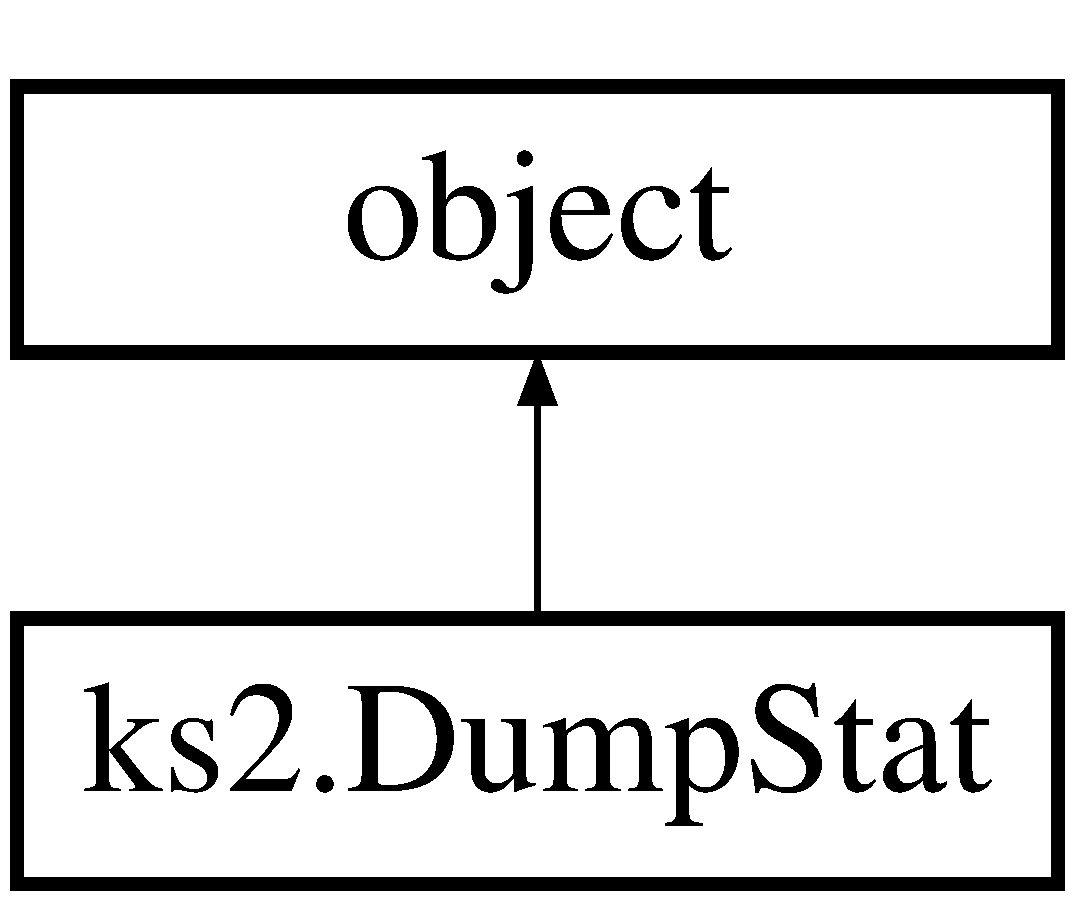
\includegraphics[height=2.000000cm]{classks2_1_1_dump_stat}
\end{center}
\end{figure}
\subsection*{Public Member Functions}
\begin{DoxyCompactItemize}
\item 
def \hyperlink{classks2_1_1_dump_stat_a58340f5ca4da0de9a01c75b2f08bdb77}{\-\_\-\-\_\-init\-\_\-\-\_\-}
\item 
def \hyperlink{classks2_1_1_dump_stat_a570d6a1b8cee2bf794873ec8ee5c67ee}{show}
\item 
def \hyperlink{classks2_1_1_dump_stat_a1f7baffa638c21cdc7bc70bf962df14d}{two\-\_\-decimal}
\end{DoxyCompactItemize}
\subsection*{Public Attributes}
\begin{DoxyCompactItemize}
\item 
\hyperlink{classks2_1_1_dump_stat_a50be5dd8149aa0879c5af8f5f46d4913}{name}
\item 
\hyperlink{classks2_1_1_dump_stat_a0ea5e91ac694afcec22e218b3b2a87d9}{xput\-\_\-min}
\item 
\hyperlink{classks2_1_1_dump_stat_aa3a7543ea60422bff1f17070f33bd10d}{xput\-\_\-max}
\item 
\hyperlink{classks2_1_1_dump_stat_a165f17a52acf19d676de78ddd079e8cf}{xput\-\_\-median}
\item 
\hyperlink{classks2_1_1_dump_stat_aff6636ea1a88d90db552b0713b3111ee}{xput\-\_\-avg}
\item 
\hyperlink{classks2_1_1_dump_stat_aa454df892cfe10f8a6eafb9913b52c10}{xput\-\_\-std}
\end{DoxyCompactItemize}


\subsection{Constructor \& Destructor Documentation}
\hypertarget{classks2_1_1_dump_stat_a58340f5ca4da0de9a01c75b2f08bdb77}{\index{ks2\-::\-Dump\-Stat@{ks2\-::\-Dump\-Stat}!\-\_\-\-\_\-init\-\_\-\-\_\-@{\-\_\-\-\_\-init\-\_\-\-\_\-}}
\index{\-\_\-\-\_\-init\-\_\-\-\_\-@{\-\_\-\-\_\-init\-\_\-\-\_\-}!ks2::DumpStat@{ks2\-::\-Dump\-Stat}}
\subsubsection[{\-\_\-\-\_\-init\-\_\-\-\_\-}]{\setlength{\rightskip}{0pt plus 5cm}def ks2.\-Dump\-Stat.\-\_\-\-\_\-init\-\_\-\-\_\- (
\begin{DoxyParamCaption}
\item[{}]{self, }
\item[{}]{xput\-\_\-min, }
\item[{}]{xput\-\_\-max, }
\item[{}]{xput\-\_\-median, }
\item[{}]{xput\-\_\-avg, }
\item[{}]{xput\-\_\-std, }
\item[{}]{name = {\ttfamily None}}
\end{DoxyParamCaption}
)}}\label{classks2_1_1_dump_stat_a58340f5ca4da0de9a01c75b2f08bdb77}


\subsection{Member Function Documentation}
\hypertarget{classks2_1_1_dump_stat_a570d6a1b8cee2bf794873ec8ee5c67ee}{\index{ks2\-::\-Dump\-Stat@{ks2\-::\-Dump\-Stat}!show@{show}}
\index{show@{show}!ks2::DumpStat@{ks2\-::\-Dump\-Stat}}
\subsubsection[{show}]{\setlength{\rightskip}{0pt plus 5cm}def ks2.\-Dump\-Stat.\-show (
\begin{DoxyParamCaption}
\item[{}]{self, }
\item[{}]{row = {\ttfamily False}}
\end{DoxyParamCaption}
)}}\label{classks2_1_1_dump_stat_a570d6a1b8cee2bf794873ec8ee5c67ee}
\hypertarget{classks2_1_1_dump_stat_a1f7baffa638c21cdc7bc70bf962df14d}{\index{ks2\-::\-Dump\-Stat@{ks2\-::\-Dump\-Stat}!two\-\_\-decimal@{two\-\_\-decimal}}
\index{two\-\_\-decimal@{two\-\_\-decimal}!ks2::DumpStat@{ks2\-::\-Dump\-Stat}}
\subsubsection[{two\-\_\-decimal}]{\setlength{\rightskip}{0pt plus 5cm}def ks2.\-Dump\-Stat.\-two\-\_\-decimal (
\begin{DoxyParamCaption}
\item[{}]{self}
\end{DoxyParamCaption}
)}}\label{classks2_1_1_dump_stat_a1f7baffa638c21cdc7bc70bf962df14d}


\subsection{Member Data Documentation}
\hypertarget{classks2_1_1_dump_stat_a50be5dd8149aa0879c5af8f5f46d4913}{\index{ks2\-::\-Dump\-Stat@{ks2\-::\-Dump\-Stat}!name@{name}}
\index{name@{name}!ks2::DumpStat@{ks2\-::\-Dump\-Stat}}
\subsubsection[{name}]{\setlength{\rightskip}{0pt plus 5cm}ks2.\-Dump\-Stat.\-name}}\label{classks2_1_1_dump_stat_a50be5dd8149aa0879c5af8f5f46d4913}
\hypertarget{classks2_1_1_dump_stat_aff6636ea1a88d90db552b0713b3111ee}{\index{ks2\-::\-Dump\-Stat@{ks2\-::\-Dump\-Stat}!xput\-\_\-avg@{xput\-\_\-avg}}
\index{xput\-\_\-avg@{xput\-\_\-avg}!ks2::DumpStat@{ks2\-::\-Dump\-Stat}}
\subsubsection[{xput\-\_\-avg}]{\setlength{\rightskip}{0pt plus 5cm}ks2.\-Dump\-Stat.\-xput\-\_\-avg}}\label{classks2_1_1_dump_stat_aff6636ea1a88d90db552b0713b3111ee}
\hypertarget{classks2_1_1_dump_stat_aa3a7543ea60422bff1f17070f33bd10d}{\index{ks2\-::\-Dump\-Stat@{ks2\-::\-Dump\-Stat}!xput\-\_\-max@{xput\-\_\-max}}
\index{xput\-\_\-max@{xput\-\_\-max}!ks2::DumpStat@{ks2\-::\-Dump\-Stat}}
\subsubsection[{xput\-\_\-max}]{\setlength{\rightskip}{0pt plus 5cm}ks2.\-Dump\-Stat.\-xput\-\_\-max}}\label{classks2_1_1_dump_stat_aa3a7543ea60422bff1f17070f33bd10d}
\hypertarget{classks2_1_1_dump_stat_a165f17a52acf19d676de78ddd079e8cf}{\index{ks2\-::\-Dump\-Stat@{ks2\-::\-Dump\-Stat}!xput\-\_\-median@{xput\-\_\-median}}
\index{xput\-\_\-median@{xput\-\_\-median}!ks2::DumpStat@{ks2\-::\-Dump\-Stat}}
\subsubsection[{xput\-\_\-median}]{\setlength{\rightskip}{0pt plus 5cm}ks2.\-Dump\-Stat.\-xput\-\_\-median}}\label{classks2_1_1_dump_stat_a165f17a52acf19d676de78ddd079e8cf}
\hypertarget{classks2_1_1_dump_stat_a0ea5e91ac694afcec22e218b3b2a87d9}{\index{ks2\-::\-Dump\-Stat@{ks2\-::\-Dump\-Stat}!xput\-\_\-min@{xput\-\_\-min}}
\index{xput\-\_\-min@{xput\-\_\-min}!ks2::DumpStat@{ks2\-::\-Dump\-Stat}}
\subsubsection[{xput\-\_\-min}]{\setlength{\rightskip}{0pt plus 5cm}ks2.\-Dump\-Stat.\-xput\-\_\-min}}\label{classks2_1_1_dump_stat_a0ea5e91ac694afcec22e218b3b2a87d9}
\hypertarget{classks2_1_1_dump_stat_aa454df892cfe10f8a6eafb9913b52c10}{\index{ks2\-::\-Dump\-Stat@{ks2\-::\-Dump\-Stat}!xput\-\_\-std@{xput\-\_\-std}}
\index{xput\-\_\-std@{xput\-\_\-std}!ks2::DumpStat@{ks2\-::\-Dump\-Stat}}
\subsubsection[{xput\-\_\-std}]{\setlength{\rightskip}{0pt plus 5cm}ks2.\-Dump\-Stat.\-xput\-\_\-std}}\label{classks2_1_1_dump_stat_aa454df892cfe10f8a6eafb9913b52c10}


The documentation for this class was generated from the following file\-:\begin{DoxyCompactItemize}
\item 
\hyperlink{ks2_8py}{ks2.\-py}\end{DoxyCompactItemize}

\hypertarget{classpython__lib_1_1_instance}{\section{python\-\_\-lib.\-Instance Class Reference}
\label{classpython__lib_1_1_instance}\index{python\-\_\-lib.\-Instance@{python\-\_\-lib.\-Instance}}
}
Inheritance diagram for python\-\_\-lib.\-Instance\-:\begin{figure}[H]
\begin{center}
\leavevmode
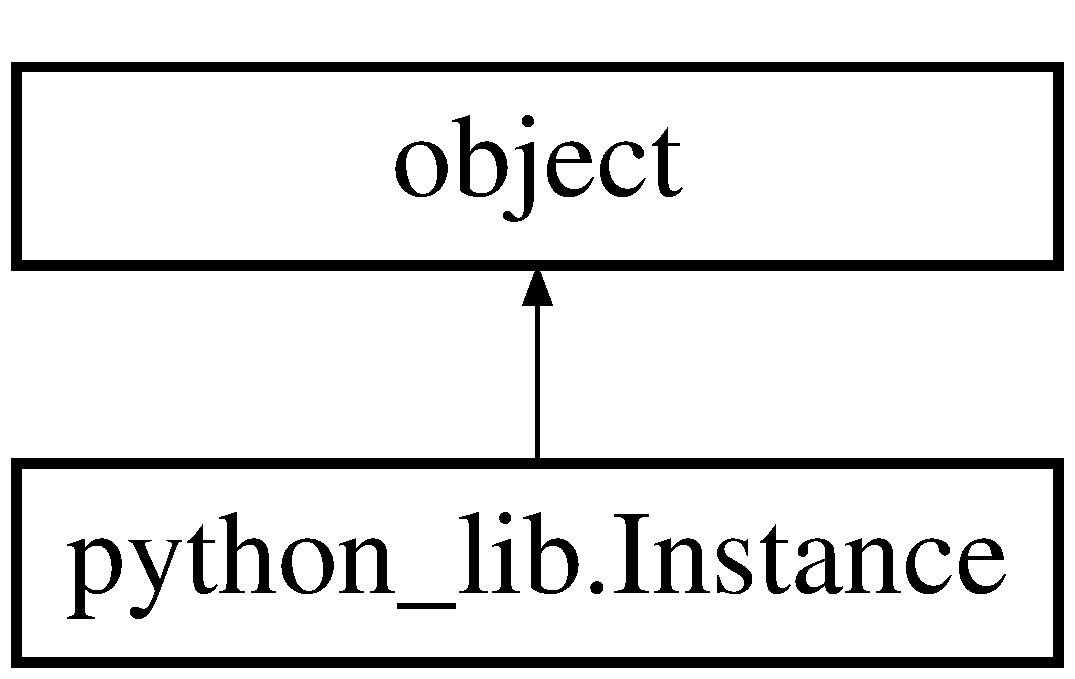
\includegraphics[height=2.000000cm]{classpython__lib_1_1_instance}
\end{center}
\end{figure}
\subsection*{Public Member Functions}
\begin{DoxyCompactItemize}
\item 
def \hyperlink{classpython__lib_1_1_instance_ad30bfb8274bcf446597ca8e947da6ae0}{\-\_\-\-\_\-init\-\_\-\-\_\-}
\item 
def \hyperlink{classpython__lib_1_1_instance_a48d1e6fbbceb1898fbfd74ad4374d829}{show}
\end{DoxyCompactItemize}
\subsection*{Public Attributes}
\begin{DoxyCompactItemize}
\item 
\hyperlink{classpython__lib_1_1_instance_a0fd04ce14016b7d0856233f490503ab9}{name}
\item 
\hyperlink{classpython__lib_1_1_instance_a313b98cd096f7ec75211979440ea7b12}{host}
\item 
\hyperlink{classpython__lib_1_1_instance_a425ff7c7985f4f5c0ceee7dd763db9e2}{username}
\item 
\hyperlink{classpython__lib_1_1_instance_af626e75528d2014eba57f2f158b99e93}{ssh\-\_\-key}
\end{DoxyCompactItemize}
\subsection*{Static Public Attributes}
\begin{DoxyCompactItemize}
\item 
dictionary \hyperlink{classpython__lib_1_1_instance_a27fea834047432419ffc36fea953b1bb}{instance\-\_\-list}
\end{DoxyCompactItemize}


\subsection{Constructor \& Destructor Documentation}
\hypertarget{classpython__lib_1_1_instance_ad30bfb8274bcf446597ca8e947da6ae0}{\index{python\-\_\-lib\-::\-Instance@{python\-\_\-lib\-::\-Instance}!\-\_\-\-\_\-init\-\_\-\-\_\-@{\-\_\-\-\_\-init\-\_\-\-\_\-}}
\index{\-\_\-\-\_\-init\-\_\-\-\_\-@{\-\_\-\-\_\-init\-\_\-\-\_\-}!python_lib::Instance@{python\-\_\-lib\-::\-Instance}}
\subsubsection[{\-\_\-\-\_\-init\-\_\-\-\_\-}]{\setlength{\rightskip}{0pt plus 5cm}def python\-\_\-lib.\-Instance.\-\_\-\-\_\-init\-\_\-\-\_\- (
\begin{DoxyParamCaption}
\item[{}]{self, }
\item[{}]{instance, }
\item[{}]{instances = {\ttfamily {\bf instance\-\_\-list}}}
\end{DoxyParamCaption}
)}}\label{classpython__lib_1_1_instance_ad30bfb8274bcf446597ca8e947da6ae0}


\subsection{Member Function Documentation}
\hypertarget{classpython__lib_1_1_instance_a48d1e6fbbceb1898fbfd74ad4374d829}{\index{python\-\_\-lib\-::\-Instance@{python\-\_\-lib\-::\-Instance}!show@{show}}
\index{show@{show}!python_lib::Instance@{python\-\_\-lib\-::\-Instance}}
\subsubsection[{show}]{\setlength{\rightskip}{0pt plus 5cm}def python\-\_\-lib.\-Instance.\-show (
\begin{DoxyParamCaption}
\item[{}]{self}
\end{DoxyParamCaption}
)}}\label{classpython__lib_1_1_instance_a48d1e6fbbceb1898fbfd74ad4374d829}


\subsection{Member Data Documentation}
\hypertarget{classpython__lib_1_1_instance_a313b98cd096f7ec75211979440ea7b12}{\index{python\-\_\-lib\-::\-Instance@{python\-\_\-lib\-::\-Instance}!host@{host}}
\index{host@{host}!python_lib::Instance@{python\-\_\-lib\-::\-Instance}}
\subsubsection[{host}]{\setlength{\rightskip}{0pt plus 5cm}python\-\_\-lib.\-Instance.\-host}}\label{classpython__lib_1_1_instance_a313b98cd096f7ec75211979440ea7b12}
\hypertarget{classpython__lib_1_1_instance_a27fea834047432419ffc36fea953b1bb}{\index{python\-\_\-lib\-::\-Instance@{python\-\_\-lib\-::\-Instance}!instance\-\_\-list@{instance\-\_\-list}}
\index{instance\-\_\-list@{instance\-\_\-list}!python_lib::Instance@{python\-\_\-lib\-::\-Instance}}
\subsubsection[{instance\-\_\-list}]{\setlength{\rightskip}{0pt plus 5cm}dictionary python\-\_\-lib.\-Instance.\-instance\-\_\-list\hspace{0.3cm}{\ttfamily [static]}}}\label{classpython__lib_1_1_instance_a27fea834047432419ffc36fea953b1bb}
{\bfseries Initial value\-:}
\begin{DoxyCode}
1 = \{
2                      \textcolor{stringliteral}{'meddle'}  : \{\textcolor{stringliteral}{'host'}     : \textcolor{stringliteral}{'ec2-54-243-17-203.compute-1.amazonaws.com'},
3                                   \textcolor{stringliteral}{'username'} : \textcolor{stringliteral}{'ubuntu'},
4                                   \textcolor{stringliteral}{'ssh\_key'}  : \textcolor{stringliteral}{'~/.ssh/meddle'}\},
5                      \textcolor{stringliteral}{'achtung'} : \{\textcolor{stringliteral}{'host'}     :\textcolor{stringliteral}{'129.10.115.141'},
6                                   \textcolor{stringliteral}{'username'} : \textcolor{stringliteral}{'arash'},
7                                   \textcolor{stringliteral}{'ssh\_key'}  : \textcolor{stringliteral}{'~/.ssh/id\_rsa'}\},
8                      \textcolor{stringliteral}{'alan-ec2'}: \{\textcolor{stringliteral}{'host'}     :\textcolor{stringliteral}{'ec2-54-204-220-73.compute-1.amazonaws.com'},
9                                   \textcolor{stringliteral}{'username'} : \textcolor{stringliteral}{'ubuntu'},
10                                   \textcolor{stringliteral}{'ssh\_key'}  : \textcolor{stringliteral}{'~/.ssh/ancsaaa-keypair\_ec2.pem'}\},
11                      \}
\end{DoxyCode}
\hypertarget{classpython__lib_1_1_instance_a0fd04ce14016b7d0856233f490503ab9}{\index{python\-\_\-lib\-::\-Instance@{python\-\_\-lib\-::\-Instance}!name@{name}}
\index{name@{name}!python_lib::Instance@{python\-\_\-lib\-::\-Instance}}
\subsubsection[{name}]{\setlength{\rightskip}{0pt plus 5cm}python\-\_\-lib.\-Instance.\-name}}\label{classpython__lib_1_1_instance_a0fd04ce14016b7d0856233f490503ab9}
\hypertarget{classpython__lib_1_1_instance_af626e75528d2014eba57f2f158b99e93}{\index{python\-\_\-lib\-::\-Instance@{python\-\_\-lib\-::\-Instance}!ssh\-\_\-key@{ssh\-\_\-key}}
\index{ssh\-\_\-key@{ssh\-\_\-key}!python_lib::Instance@{python\-\_\-lib\-::\-Instance}}
\subsubsection[{ssh\-\_\-key}]{\setlength{\rightskip}{0pt plus 5cm}python\-\_\-lib.\-Instance.\-ssh\-\_\-key}}\label{classpython__lib_1_1_instance_af626e75528d2014eba57f2f158b99e93}
\hypertarget{classpython__lib_1_1_instance_a425ff7c7985f4f5c0ceee7dd763db9e2}{\index{python\-\_\-lib\-::\-Instance@{python\-\_\-lib\-::\-Instance}!username@{username}}
\index{username@{username}!python_lib::Instance@{python\-\_\-lib\-::\-Instance}}
\subsubsection[{username}]{\setlength{\rightskip}{0pt plus 5cm}python\-\_\-lib.\-Instance.\-username}}\label{classpython__lib_1_1_instance_a425ff7c7985f4f5c0ceee7dd763db9e2}


The documentation for this class was generated from the following file\-:\begin{DoxyCompactItemize}
\item 
\hyperlink{python__lib_8py}{python\-\_\-lib.\-py}\end{DoxyCompactItemize}

\hypertarget{classtornado__server_1_1_main_handler}{\section{tornado\-\_\-server.\-Main\-Handler Class Reference}
\label{classtornado__server_1_1_main_handler}\index{tornado\-\_\-server.\-Main\-Handler@{tornado\-\_\-server.\-Main\-Handler}}
}
Inheritance diagram for tornado\-\_\-server.\-Main\-Handler\-:\begin{figure}[H]
\begin{center}
\leavevmode
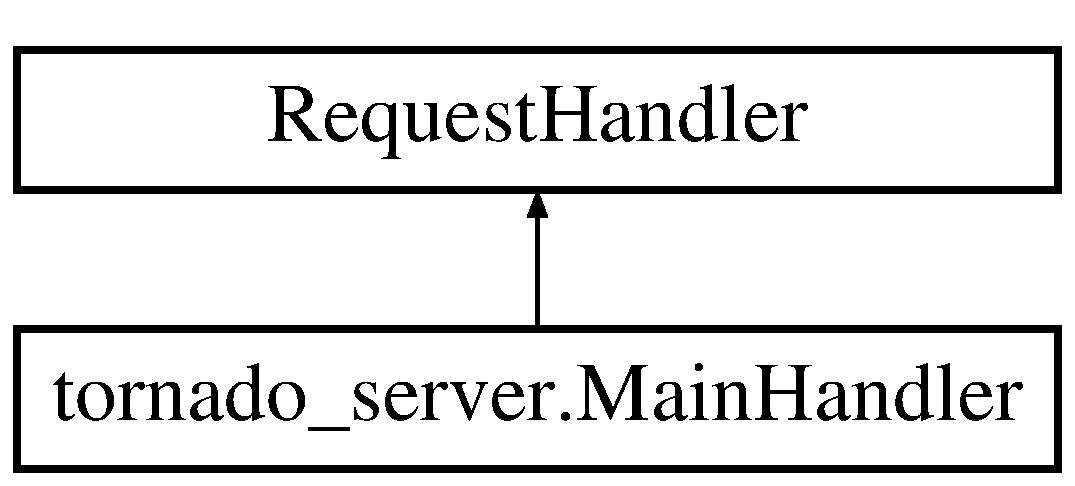
\includegraphics[height=2.000000cm]{classtornado__server_1_1_main_handler}
\end{center}
\end{figure}
\subsection*{Public Member Functions}
\begin{DoxyCompactItemize}
\item 
def \hyperlink{classtornado__server_1_1_main_handler_a4d658d7ed066245516cf4e8014839baf}{get}
\end{DoxyCompactItemize}


\subsection{Member Function Documentation}
\hypertarget{classtornado__server_1_1_main_handler_a4d658d7ed066245516cf4e8014839baf}{\index{tornado\-\_\-server\-::\-Main\-Handler@{tornado\-\_\-server\-::\-Main\-Handler}!get@{get}}
\index{get@{get}!tornado_server::MainHandler@{tornado\-\_\-server\-::\-Main\-Handler}}
\subsubsection[{get}]{\setlength{\rightskip}{0pt plus 5cm}def tornado\-\_\-server.\-Main\-Handler.\-get (
\begin{DoxyParamCaption}
\item[{}]{self}
\end{DoxyParamCaption}
)}}\label{classtornado__server_1_1_main_handler_a4d658d7ed066245516cf4e8014839baf}


The documentation for this class was generated from the following file\-:\begin{DoxyCompactItemize}
\item 
\hyperlink{tornado__server_8py}{tornado\-\_\-server.\-py}\end{DoxyCompactItemize}

\hypertarget{classpython__lib_1_1_one_response}{\section{python\-\_\-lib.\-One\-Response Class Reference}
\label{classpython__lib_1_1_one_response}\index{python\-\_\-lib.\-One\-Response@{python\-\_\-lib.\-One\-Response}}
}
Inheritance diagram for python\-\_\-lib.\-One\-Response\-:\begin{figure}[H]
\begin{center}
\leavevmode
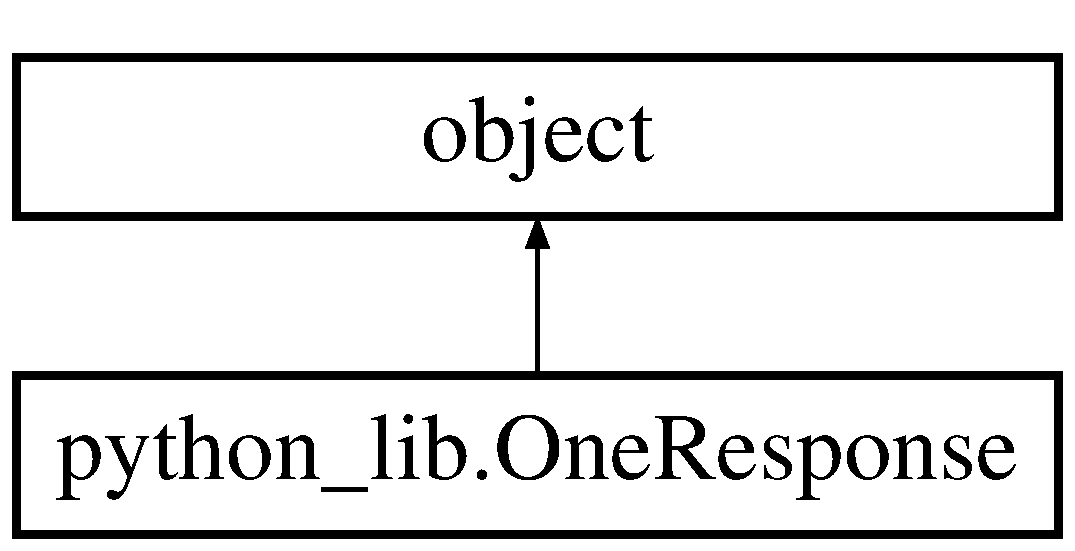
\includegraphics[height=2.000000cm]{classpython__lib_1_1_one_response}
\end{center}
\end{figure}
\subsection*{Public Member Functions}
\begin{DoxyCompactItemize}
\item 
def \hyperlink{classpython__lib_1_1_one_response_aebfa88bda9e981a4bc1cb3423776c5b4}{\-\_\-\-\_\-init\-\_\-\-\_\-}
\end{DoxyCompactItemize}
\subsection*{Public Attributes}
\begin{DoxyCompactItemize}
\item 
\hyperlink{classpython__lib_1_1_one_response_a33490413e76a4b92c0d947875c553cf0}{payload}
\item 
\hyperlink{classpython__lib_1_1_one_response_a1c5706bab79abb280fb0a46e3ea65d32}{timestamp}
\end{DoxyCompactItemize}


\subsection{Constructor \& Destructor Documentation}
\hypertarget{classpython__lib_1_1_one_response_aebfa88bda9e981a4bc1cb3423776c5b4}{\index{python\-\_\-lib\-::\-One\-Response@{python\-\_\-lib\-::\-One\-Response}!\-\_\-\-\_\-init\-\_\-\-\_\-@{\-\_\-\-\_\-init\-\_\-\-\_\-}}
\index{\-\_\-\-\_\-init\-\_\-\-\_\-@{\-\_\-\-\_\-init\-\_\-\-\_\-}!python_lib::OneResponse@{python\-\_\-lib\-::\-One\-Response}}
\subsubsection[{\-\_\-\-\_\-init\-\_\-\-\_\-}]{\setlength{\rightskip}{0pt plus 5cm}def python\-\_\-lib.\-One\-Response.\-\_\-\-\_\-init\-\_\-\-\_\- (
\begin{DoxyParamCaption}
\item[{}]{self, }
\item[{}]{payload, }
\item[{}]{timestamp}
\end{DoxyParamCaption}
)}}\label{classpython__lib_1_1_one_response_aebfa88bda9e981a4bc1cb3423776c5b4}


\subsection{Member Data Documentation}
\hypertarget{classpython__lib_1_1_one_response_a33490413e76a4b92c0d947875c553cf0}{\index{python\-\_\-lib\-::\-One\-Response@{python\-\_\-lib\-::\-One\-Response}!payload@{payload}}
\index{payload@{payload}!python_lib::OneResponse@{python\-\_\-lib\-::\-One\-Response}}
\subsubsection[{payload}]{\setlength{\rightskip}{0pt plus 5cm}python\-\_\-lib.\-One\-Response.\-payload}}\label{classpython__lib_1_1_one_response_a33490413e76a4b92c0d947875c553cf0}
\hypertarget{classpython__lib_1_1_one_response_a1c5706bab79abb280fb0a46e3ea65d32}{\index{python\-\_\-lib\-::\-One\-Response@{python\-\_\-lib\-::\-One\-Response}!timestamp@{timestamp}}
\index{timestamp@{timestamp}!python_lib::OneResponse@{python\-\_\-lib\-::\-One\-Response}}
\subsubsection[{timestamp}]{\setlength{\rightskip}{0pt plus 5cm}python\-\_\-lib.\-One\-Response.\-timestamp}}\label{classpython__lib_1_1_one_response_a1c5706bab79abb280fb0a46e3ea65d32}


The documentation for this class was generated from the following file\-:\begin{DoxyCompactItemize}
\item 
\hyperlink{python__lib_8py}{python\-\_\-lib.\-py}\end{DoxyCompactItemize}

\hypertarget{classtcp__client_1_1_queue}{\section{tcp\-\_\-client.\-Queue Class Reference}
\label{classtcp__client_1_1_queue}\index{tcp\-\_\-client.\-Queue@{tcp\-\_\-client.\-Queue}}
}
Inheritance diagram for tcp\-\_\-client.\-Queue\-:\begin{figure}[H]
\begin{center}
\leavevmode
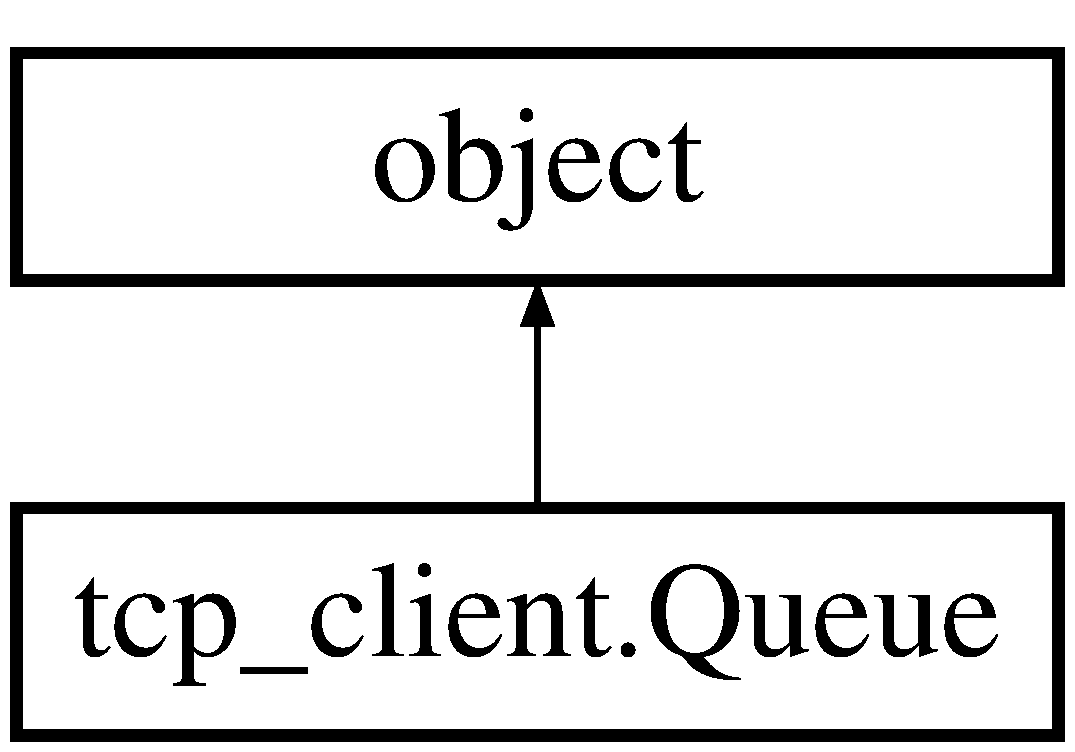
\includegraphics[height=2.000000cm]{classtcp__client_1_1_queue}
\end{center}
\end{figure}
\subsection*{Public Member Functions}
\begin{DoxyCompactItemize}
\item 
def \hyperlink{classtcp__client_1_1_queue_ab0df6abd257ea9a0ed489b519d0a3be8}{\-\_\-\-\_\-init\-\_\-\-\_\-}
\item 
def \hyperlink{classtcp__client_1_1_queue_ae86fb384d543cc9546ba747033995b8e}{next}
\item 
def \hyperlink{classtcp__client_1_1_queue_a0ad188422dd352a1cfecd4b73c63e719}{run}
\end{DoxyCompactItemize}
\subsection*{Public Attributes}
\begin{DoxyCompactItemize}
\item 
\hyperlink{classtcp__client_1_1_queue_ad1d79a3f78925181c48bae6c7fee899d}{Q}
\item 
\hyperlink{classtcp__client_1_1_queue_a0843d2bd2c1a7e5e237c2948fa1247e6}{event}
\item 
\hyperlink{classtcp__client_1_1_queue_ad872c06b7212edb7df8adbf02f77eb50}{waitlist}
\item 
\hyperlink{classtcp__client_1_1_queue_a7d5e8ff7e6e26fc8a0914872547b6690}{sendlist}
\item 
\hyperlink{classtcp__client_1_1_queue_a8030358b15948a4260c5a41661982622}{time\-\_\-origin}
\item 
\hyperlink{classtcp__client_1_1_queue_aea5f1243cbc1d111dfa33578426e2591}{connections}
\end{DoxyCompactItemize}


\subsection{Detailed Description}
\begin{DoxyVerb}This is the class which sends out the packets in the queue one-by-one.
Before sending any packets, it makes sure:
    1- All previous packets are sent
    2- All previous responses on the same connection are recieved
    3- Packet time has passed
Once all the above are satisfied, it fires of a thread with traget = SendRecv().send_single_request
\end{DoxyVerb}
 

\subsection{Constructor \& Destructor Documentation}
\hypertarget{classtcp__client_1_1_queue_ab0df6abd257ea9a0ed489b519d0a3be8}{\index{tcp\-\_\-client\-::\-Queue@{tcp\-\_\-client\-::\-Queue}!\-\_\-\-\_\-init\-\_\-\-\_\-@{\-\_\-\-\_\-init\-\_\-\-\_\-}}
\index{\-\_\-\-\_\-init\-\_\-\-\_\-@{\-\_\-\-\_\-init\-\_\-\-\_\-}!tcp_client::Queue@{tcp\-\_\-client\-::\-Queue}}
\subsubsection[{\-\_\-\-\_\-init\-\_\-\-\_\-}]{\setlength{\rightskip}{0pt plus 5cm}def tcp\-\_\-client.\-Queue.\-\_\-\-\_\-init\-\_\-\-\_\- (
\begin{DoxyParamCaption}
\item[{}]{self, }
\item[{}]{queue}
\end{DoxyParamCaption}
)}}\label{classtcp__client_1_1_queue_ab0df6abd257ea9a0ed489b519d0a3be8}


\subsection{Member Function Documentation}
\hypertarget{classtcp__client_1_1_queue_ae86fb384d543cc9546ba747033995b8e}{\index{tcp\-\_\-client\-::\-Queue@{tcp\-\_\-client\-::\-Queue}!next@{next}}
\index{next@{next}!tcp_client::Queue@{tcp\-\_\-client\-::\-Queue}}
\subsubsection[{next}]{\setlength{\rightskip}{0pt plus 5cm}def tcp\-\_\-client.\-Queue.\-next (
\begin{DoxyParamCaption}
\item[{}]{self}
\end{DoxyParamCaption}
)}}\label{classtcp__client_1_1_queue_ae86fb384d543cc9546ba747033995b8e}
\hypertarget{classtcp__client_1_1_queue_a0ad188422dd352a1cfecd4b73c63e719}{\index{tcp\-\_\-client\-::\-Queue@{tcp\-\_\-client\-::\-Queue}!run@{run}}
\index{run@{run}!tcp_client::Queue@{tcp\-\_\-client\-::\-Queue}}
\subsubsection[{run}]{\setlength{\rightskip}{0pt plus 5cm}def tcp\-\_\-client.\-Queue.\-run (
\begin{DoxyParamCaption}
\item[{}]{self}
\end{DoxyParamCaption}
)}}\label{classtcp__client_1_1_queue_a0ad188422dd352a1cfecd4b73c63e719}


\subsection{Member Data Documentation}
\hypertarget{classtcp__client_1_1_queue_aea5f1243cbc1d111dfa33578426e2591}{\index{tcp\-\_\-client\-::\-Queue@{tcp\-\_\-client\-::\-Queue}!connections@{connections}}
\index{connections@{connections}!tcp_client::Queue@{tcp\-\_\-client\-::\-Queue}}
\subsubsection[{connections}]{\setlength{\rightskip}{0pt plus 5cm}tcp\-\_\-client.\-Queue.\-connections}}\label{classtcp__client_1_1_queue_aea5f1243cbc1d111dfa33578426e2591}
\hypertarget{classtcp__client_1_1_queue_a0843d2bd2c1a7e5e237c2948fa1247e6}{\index{tcp\-\_\-client\-::\-Queue@{tcp\-\_\-client\-::\-Queue}!event@{event}}
\index{event@{event}!tcp_client::Queue@{tcp\-\_\-client\-::\-Queue}}
\subsubsection[{event}]{\setlength{\rightskip}{0pt plus 5cm}tcp\-\_\-client.\-Queue.\-event}}\label{classtcp__client_1_1_queue_a0843d2bd2c1a7e5e237c2948fa1247e6}
\hypertarget{classtcp__client_1_1_queue_ad1d79a3f78925181c48bae6c7fee899d}{\index{tcp\-\_\-client\-::\-Queue@{tcp\-\_\-client\-::\-Queue}!Q@{Q}}
\index{Q@{Q}!tcp_client::Queue@{tcp\-\_\-client\-::\-Queue}}
\subsubsection[{Q}]{\setlength{\rightskip}{0pt plus 5cm}tcp\-\_\-client.\-Queue.\-Q}}\label{classtcp__client_1_1_queue_ad1d79a3f78925181c48bae6c7fee899d}
\hypertarget{classtcp__client_1_1_queue_a7d5e8ff7e6e26fc8a0914872547b6690}{\index{tcp\-\_\-client\-::\-Queue@{tcp\-\_\-client\-::\-Queue}!sendlist@{sendlist}}
\index{sendlist@{sendlist}!tcp_client::Queue@{tcp\-\_\-client\-::\-Queue}}
\subsubsection[{sendlist}]{\setlength{\rightskip}{0pt plus 5cm}tcp\-\_\-client.\-Queue.\-sendlist}}\label{classtcp__client_1_1_queue_a7d5e8ff7e6e26fc8a0914872547b6690}
\hypertarget{classtcp__client_1_1_queue_a8030358b15948a4260c5a41661982622}{\index{tcp\-\_\-client\-::\-Queue@{tcp\-\_\-client\-::\-Queue}!time\-\_\-origin@{time\-\_\-origin}}
\index{time\-\_\-origin@{time\-\_\-origin}!tcp_client::Queue@{tcp\-\_\-client\-::\-Queue}}
\subsubsection[{time\-\_\-origin}]{\setlength{\rightskip}{0pt plus 5cm}tcp\-\_\-client.\-Queue.\-time\-\_\-origin}}\label{classtcp__client_1_1_queue_a8030358b15948a4260c5a41661982622}
\hypertarget{classtcp__client_1_1_queue_ad872c06b7212edb7df8adbf02f77eb50}{\index{tcp\-\_\-client\-::\-Queue@{tcp\-\_\-client\-::\-Queue}!waitlist@{waitlist}}
\index{waitlist@{waitlist}!tcp_client::Queue@{tcp\-\_\-client\-::\-Queue}}
\subsubsection[{waitlist}]{\setlength{\rightskip}{0pt plus 5cm}tcp\-\_\-client.\-Queue.\-waitlist}}\label{classtcp__client_1_1_queue_ad872c06b7212edb7df8adbf02f77eb50}


The documentation for this class was generated from the following file\-:\begin{DoxyCompactItemize}
\item 
\hyperlink{tcp__client_8py}{tcp\-\_\-client.\-py}\end{DoxyCompactItemize}

\hypertarget{classtornado__server_1_1_record_replay}{\section{tornado\-\_\-server.\-Record\-Replay Class Reference}
\label{classtornado__server_1_1_record_replay}\index{tornado\-\_\-server.\-Record\-Replay@{tornado\-\_\-server.\-Record\-Replay}}
}
Inheritance diagram for tornado\-\_\-server.\-Record\-Replay\-:\begin{figure}[H]
\begin{center}
\leavevmode
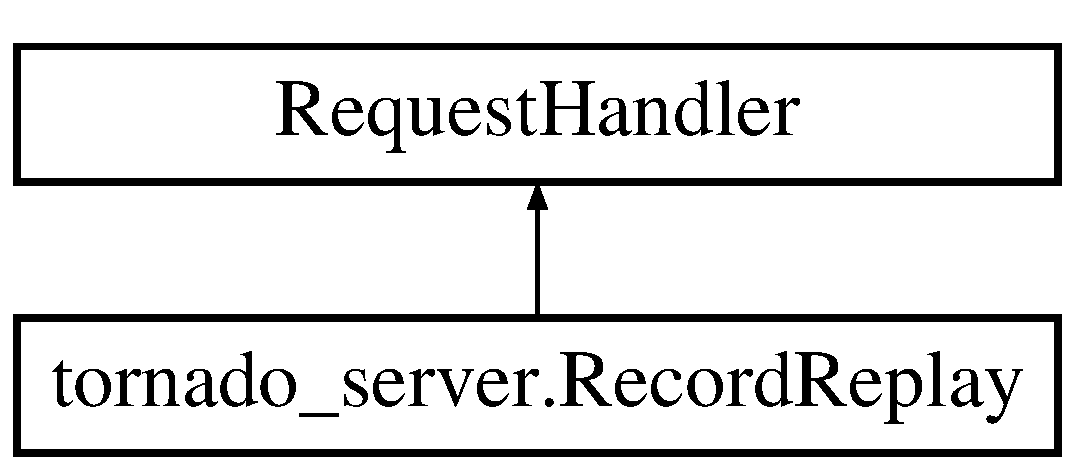
\includegraphics[height=2.000000cm]{classtornado__server_1_1_record_replay}
\end{center}
\end{figure}
\subsection*{Public Member Functions}
\begin{DoxyCompactItemize}
\item 
def \hyperlink{classtornado__server_1_1_record_replay_a28cbc3f105e972e3e324e133407caa0b}{get}
\end{DoxyCompactItemize}


\subsection{Member Function Documentation}
\hypertarget{classtornado__server_1_1_record_replay_a28cbc3f105e972e3e324e133407caa0b}{\index{tornado\-\_\-server\-::\-Record\-Replay@{tornado\-\_\-server\-::\-Record\-Replay}!get@{get}}
\index{get@{get}!tornado_server::RecordReplay@{tornado\-\_\-server\-::\-Record\-Replay}}
\subsubsection[{get}]{\setlength{\rightskip}{0pt plus 5cm}def tornado\-\_\-server.\-Record\-Replay.\-get (
\begin{DoxyParamCaption}
\item[{}]{self}
\end{DoxyParamCaption}
)}}\label{classtornado__server_1_1_record_replay_a28cbc3f105e972e3e324e133407caa0b}


The documentation for this class was generated from the following file\-:\begin{DoxyCompactItemize}
\item 
\hyperlink{tornado__server_8py}{tornado\-\_\-server.\-py}\end{DoxyCompactItemize}

\hypertarget{classpython__lib_1_1_request_set}{\section{python\-\_\-lib.\-Request\-Set Class Reference}
\label{classpython__lib_1_1_request_set}\index{python\-\_\-lib.\-Request\-Set@{python\-\_\-lib.\-Request\-Set}}
}
Inheritance diagram for python\-\_\-lib.\-Request\-Set\-:\begin{figure}[H]
\begin{center}
\leavevmode
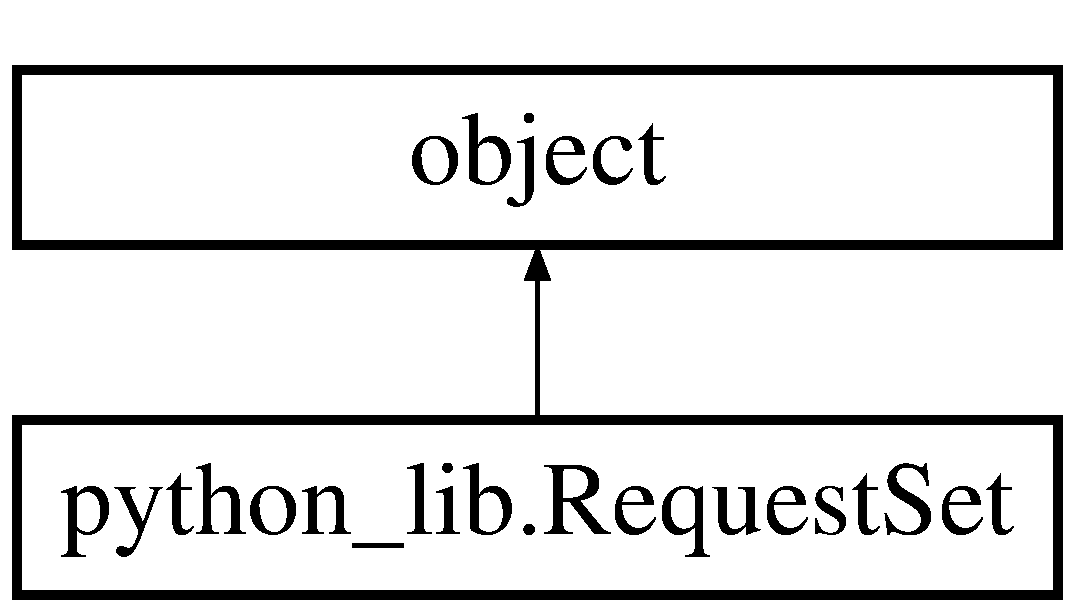
\includegraphics[height=2.000000cm]{classpython__lib_1_1_request_set}
\end{center}
\end{figure}
\subsection*{Public Member Functions}
\begin{DoxyCompactItemize}
\item 
def \hyperlink{classpython__lib_1_1_request_set_a02cf5b19c9bede07be06458eae79a544}{\-\_\-\-\_\-init\-\_\-\-\_\-}
\end{DoxyCompactItemize}
\subsection*{Public Attributes}
\begin{DoxyCompactItemize}
\item 
\hyperlink{classpython__lib_1_1_request_set_ae1fd45c566f5f08902900f335d30d4db}{payload}
\item 
\hyperlink{classpython__lib_1_1_request_set_a826cc1aaaaceb16fc03237046bab4792}{c\-\_\-s\-\_\-pair}
\item 
\hyperlink{classpython__lib_1_1_request_set_a5b22a41c3e54fa9879cffa18bc5ca65b}{response\-\_\-hash}
\item 
\hyperlink{classpython__lib_1_1_request_set_aa420f3fe719844f676b06ce5ceb67da0}{response\-\_\-len}
\item 
\hyperlink{classpython__lib_1_1_request_set_a7a93e544e11b330069fe9d5fc7ccdef3}{timestamp}
\end{DoxyCompactItemize}


\subsection{Constructor \& Destructor Documentation}
\hypertarget{classpython__lib_1_1_request_set_a02cf5b19c9bede07be06458eae79a544}{\index{python\-\_\-lib\-::\-Request\-Set@{python\-\_\-lib\-::\-Request\-Set}!\-\_\-\-\_\-init\-\_\-\-\_\-@{\-\_\-\-\_\-init\-\_\-\-\_\-}}
\index{\-\_\-\-\_\-init\-\_\-\-\_\-@{\-\_\-\-\_\-init\-\_\-\-\_\-}!python_lib::RequestSet@{python\-\_\-lib\-::\-Request\-Set}}
\subsubsection[{\-\_\-\-\_\-init\-\_\-\-\_\-}]{\setlength{\rightskip}{0pt plus 5cm}def python\-\_\-lib.\-Request\-Set.\-\_\-\-\_\-init\-\_\-\-\_\- (
\begin{DoxyParamCaption}
\item[{}]{self, }
\item[{}]{payload, }
\item[{}]{c\-\_\-s\-\_\-pair, }
\item[{}]{response, }
\item[{}]{timestamp}
\end{DoxyParamCaption}
)}}\label{classpython__lib_1_1_request_set_a02cf5b19c9bede07be06458eae79a544}


\subsection{Member Data Documentation}
\hypertarget{classpython__lib_1_1_request_set_a826cc1aaaaceb16fc03237046bab4792}{\index{python\-\_\-lib\-::\-Request\-Set@{python\-\_\-lib\-::\-Request\-Set}!c\-\_\-s\-\_\-pair@{c\-\_\-s\-\_\-pair}}
\index{c\-\_\-s\-\_\-pair@{c\-\_\-s\-\_\-pair}!python_lib::RequestSet@{python\-\_\-lib\-::\-Request\-Set}}
\subsubsection[{c\-\_\-s\-\_\-pair}]{\setlength{\rightskip}{0pt plus 5cm}python\-\_\-lib.\-Request\-Set.\-c\-\_\-s\-\_\-pair}}\label{classpython__lib_1_1_request_set_a826cc1aaaaceb16fc03237046bab4792}
\hypertarget{classpython__lib_1_1_request_set_ae1fd45c566f5f08902900f335d30d4db}{\index{python\-\_\-lib\-::\-Request\-Set@{python\-\_\-lib\-::\-Request\-Set}!payload@{payload}}
\index{payload@{payload}!python_lib::RequestSet@{python\-\_\-lib\-::\-Request\-Set}}
\subsubsection[{payload}]{\setlength{\rightskip}{0pt plus 5cm}python\-\_\-lib.\-Request\-Set.\-payload}}\label{classpython__lib_1_1_request_set_ae1fd45c566f5f08902900f335d30d4db}
\hypertarget{classpython__lib_1_1_request_set_a5b22a41c3e54fa9879cffa18bc5ca65b}{\index{python\-\_\-lib\-::\-Request\-Set@{python\-\_\-lib\-::\-Request\-Set}!response\-\_\-hash@{response\-\_\-hash}}
\index{response\-\_\-hash@{response\-\_\-hash}!python_lib::RequestSet@{python\-\_\-lib\-::\-Request\-Set}}
\subsubsection[{response\-\_\-hash}]{\setlength{\rightskip}{0pt plus 5cm}python\-\_\-lib.\-Request\-Set.\-response\-\_\-hash}}\label{classpython__lib_1_1_request_set_a5b22a41c3e54fa9879cffa18bc5ca65b}
\hypertarget{classpython__lib_1_1_request_set_aa420f3fe719844f676b06ce5ceb67da0}{\index{python\-\_\-lib\-::\-Request\-Set@{python\-\_\-lib\-::\-Request\-Set}!response\-\_\-len@{response\-\_\-len}}
\index{response\-\_\-len@{response\-\_\-len}!python_lib::RequestSet@{python\-\_\-lib\-::\-Request\-Set}}
\subsubsection[{response\-\_\-len}]{\setlength{\rightskip}{0pt plus 5cm}python\-\_\-lib.\-Request\-Set.\-response\-\_\-len}}\label{classpython__lib_1_1_request_set_aa420f3fe719844f676b06ce5ceb67da0}
\hypertarget{classpython__lib_1_1_request_set_a7a93e544e11b330069fe9d5fc7ccdef3}{\index{python\-\_\-lib\-::\-Request\-Set@{python\-\_\-lib\-::\-Request\-Set}!timestamp@{timestamp}}
\index{timestamp@{timestamp}!python_lib::RequestSet@{python\-\_\-lib\-::\-Request\-Set}}
\subsubsection[{timestamp}]{\setlength{\rightskip}{0pt plus 5cm}python\-\_\-lib.\-Request\-Set.\-timestamp}}\label{classpython__lib_1_1_request_set_a7a93e544e11b330069fe9d5fc7ccdef3}


The documentation for this class was generated from the following file\-:\begin{DoxyCompactItemize}
\item 
\hyperlink{python__lib_8py}{python\-\_\-lib.\-py}\end{DoxyCompactItemize}

\hypertarget{classtornado__server_1_1_re_run}{\section{tornado\-\_\-server.\-Re\-Run Class Reference}
\label{classtornado__server_1_1_re_run}\index{tornado\-\_\-server.\-Re\-Run@{tornado\-\_\-server.\-Re\-Run}}
}
Inheritance diagram for tornado\-\_\-server.\-Re\-Run\-:\begin{figure}[H]
\begin{center}
\leavevmode
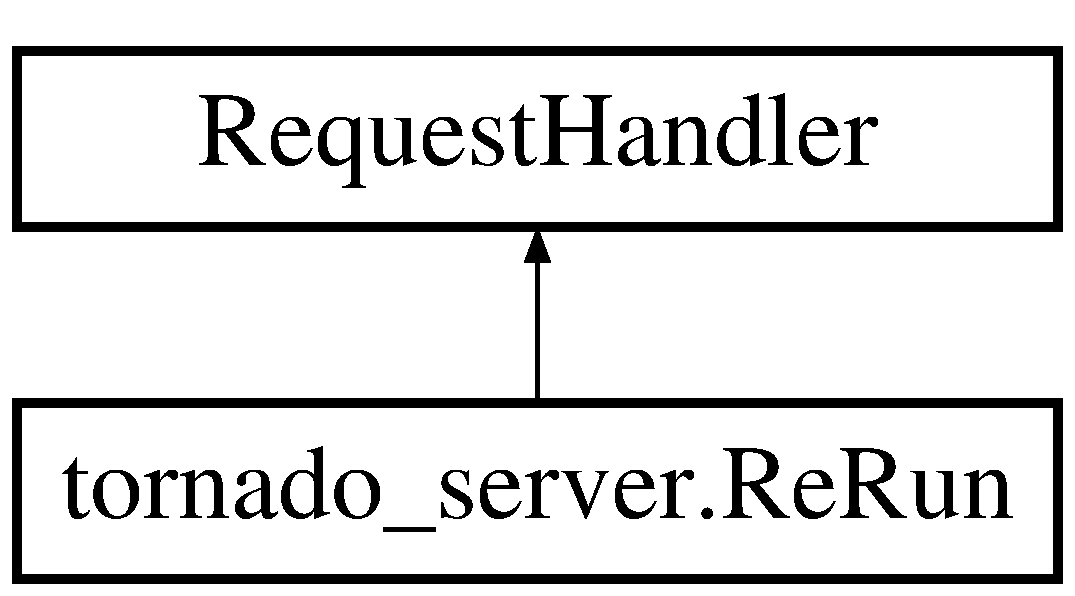
\includegraphics[height=2.000000cm]{classtornado__server_1_1_re_run}
\end{center}
\end{figure}
\subsection*{Public Member Functions}
\begin{DoxyCompactItemize}
\item 
def \hyperlink{classtornado__server_1_1_re_run_a892a278d9095adfaa5b0e4c1f560edac}{get}
\end{DoxyCompactItemize}


\subsection{Member Function Documentation}
\hypertarget{classtornado__server_1_1_re_run_a892a278d9095adfaa5b0e4c1f560edac}{\index{tornado\-\_\-server\-::\-Re\-Run@{tornado\-\_\-server\-::\-Re\-Run}!get@{get}}
\index{get@{get}!tornado_server::ReRun@{tornado\-\_\-server\-::\-Re\-Run}}
\subsubsection[{get}]{\setlength{\rightskip}{0pt plus 5cm}def tornado\-\_\-server.\-Re\-Run.\-get (
\begin{DoxyParamCaption}
\item[{}]{self}
\end{DoxyParamCaption}
)}}\label{classtornado__server_1_1_re_run_a892a278d9095adfaa5b0e4c1f560edac}


The documentation for this class was generated from the following file\-:\begin{DoxyCompactItemize}
\item 
\hyperlink{tornado__server_8py}{tornado\-\_\-server.\-py}\end{DoxyCompactItemize}

\hypertarget{classpython__lib_1_1_response_set}{\section{python\-\_\-lib.\-Response\-Set Class Reference}
\label{classpython__lib_1_1_response_set}\index{python\-\_\-lib.\-Response\-Set@{python\-\_\-lib.\-Response\-Set}}
}
Inheritance diagram for python\-\_\-lib.\-Response\-Set\-:\begin{figure}[H]
\begin{center}
\leavevmode
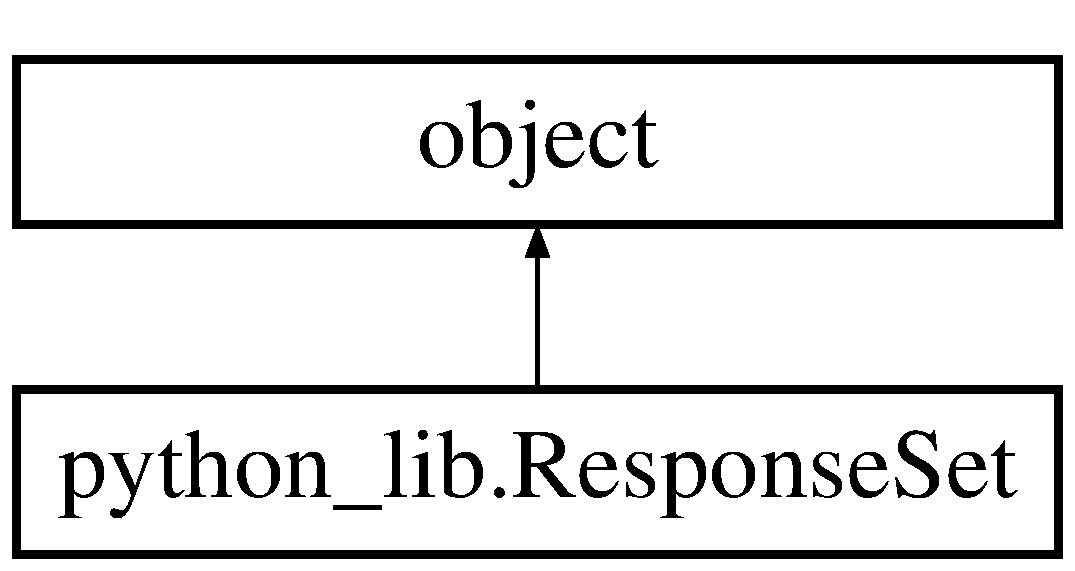
\includegraphics[height=2.000000cm]{classpython__lib_1_1_response_set}
\end{center}
\end{figure}
\subsection*{Public Member Functions}
\begin{DoxyCompactItemize}
\item 
def \hyperlink{classpython__lib_1_1_response_set_ac9490fc227817ba2aabb44e29bad3790}{\-\_\-\-\_\-init\-\_\-\-\_\-}
\end{DoxyCompactItemize}
\subsection*{Public Attributes}
\begin{DoxyCompactItemize}
\item 
\hyperlink{classpython__lib_1_1_response_set_a367476495a8153449e57c0bd7e03057f}{request\-\_\-len}
\item 
\hyperlink{classpython__lib_1_1_response_set_a8a94812ec58f4aeb8d25e7db276ffd18}{request\-\_\-hash}
\item 
\hyperlink{classpython__lib_1_1_response_set_add79790ff3d888c6660a05f97ca39f7d}{response\-\_\-list}
\end{DoxyCompactItemize}


\subsection{Constructor \& Destructor Documentation}
\hypertarget{classpython__lib_1_1_response_set_ac9490fc227817ba2aabb44e29bad3790}{\index{python\-\_\-lib\-::\-Response\-Set@{python\-\_\-lib\-::\-Response\-Set}!\-\_\-\-\_\-init\-\_\-\-\_\-@{\-\_\-\-\_\-init\-\_\-\-\_\-}}
\index{\-\_\-\-\_\-init\-\_\-\-\_\-@{\-\_\-\-\_\-init\-\_\-\-\_\-}!python_lib::ResponseSet@{python\-\_\-lib\-::\-Response\-Set}}
\subsubsection[{\-\_\-\-\_\-init\-\_\-\-\_\-}]{\setlength{\rightskip}{0pt plus 5cm}def python\-\_\-lib.\-Response\-Set.\-\_\-\-\_\-init\-\_\-\-\_\- (
\begin{DoxyParamCaption}
\item[{}]{self, }
\item[{}]{request, }
\item[{}]{response\-\_\-list}
\end{DoxyParamCaption}
)}}\label{classpython__lib_1_1_response_set_ac9490fc227817ba2aabb44e29bad3790}


\subsection{Member Data Documentation}
\hypertarget{classpython__lib_1_1_response_set_a8a94812ec58f4aeb8d25e7db276ffd18}{\index{python\-\_\-lib\-::\-Response\-Set@{python\-\_\-lib\-::\-Response\-Set}!request\-\_\-hash@{request\-\_\-hash}}
\index{request\-\_\-hash@{request\-\_\-hash}!python_lib::ResponseSet@{python\-\_\-lib\-::\-Response\-Set}}
\subsubsection[{request\-\_\-hash}]{\setlength{\rightskip}{0pt plus 5cm}python\-\_\-lib.\-Response\-Set.\-request\-\_\-hash}}\label{classpython__lib_1_1_response_set_a8a94812ec58f4aeb8d25e7db276ffd18}
\hypertarget{classpython__lib_1_1_response_set_a367476495a8153449e57c0bd7e03057f}{\index{python\-\_\-lib\-::\-Response\-Set@{python\-\_\-lib\-::\-Response\-Set}!request\-\_\-len@{request\-\_\-len}}
\index{request\-\_\-len@{request\-\_\-len}!python_lib::ResponseSet@{python\-\_\-lib\-::\-Response\-Set}}
\subsubsection[{request\-\_\-len}]{\setlength{\rightskip}{0pt plus 5cm}python\-\_\-lib.\-Response\-Set.\-request\-\_\-len}}\label{classpython__lib_1_1_response_set_a367476495a8153449e57c0bd7e03057f}
\hypertarget{classpython__lib_1_1_response_set_add79790ff3d888c6660a05f97ca39f7d}{\index{python\-\_\-lib\-::\-Response\-Set@{python\-\_\-lib\-::\-Response\-Set}!response\-\_\-list@{response\-\_\-list}}
\index{response\-\_\-list@{response\-\_\-list}!python_lib::ResponseSet@{python\-\_\-lib\-::\-Response\-Set}}
\subsubsection[{response\-\_\-list}]{\setlength{\rightskip}{0pt plus 5cm}python\-\_\-lib.\-Response\-Set.\-response\-\_\-list}}\label{classpython__lib_1_1_response_set_add79790ff3d888c6660a05f97ca39f7d}


The documentation for this class was generated from the following file\-:\begin{DoxyCompactItemize}
\item 
\hyperlink{python__lib_8py}{python\-\_\-lib.\-py}\end{DoxyCompactItemize}

\hypertarget{classtcp__client_1_1_send_recv}{\section{tcp\-\_\-client.\-Send\-Recv Class Reference}
\label{classtcp__client_1_1_send_recv}\index{tcp\-\_\-client.\-Send\-Recv@{tcp\-\_\-client.\-Send\-Recv}}
}
Inheritance diagram for tcp\-\_\-client.\-Send\-Recv\-:\begin{figure}[H]
\begin{center}
\leavevmode
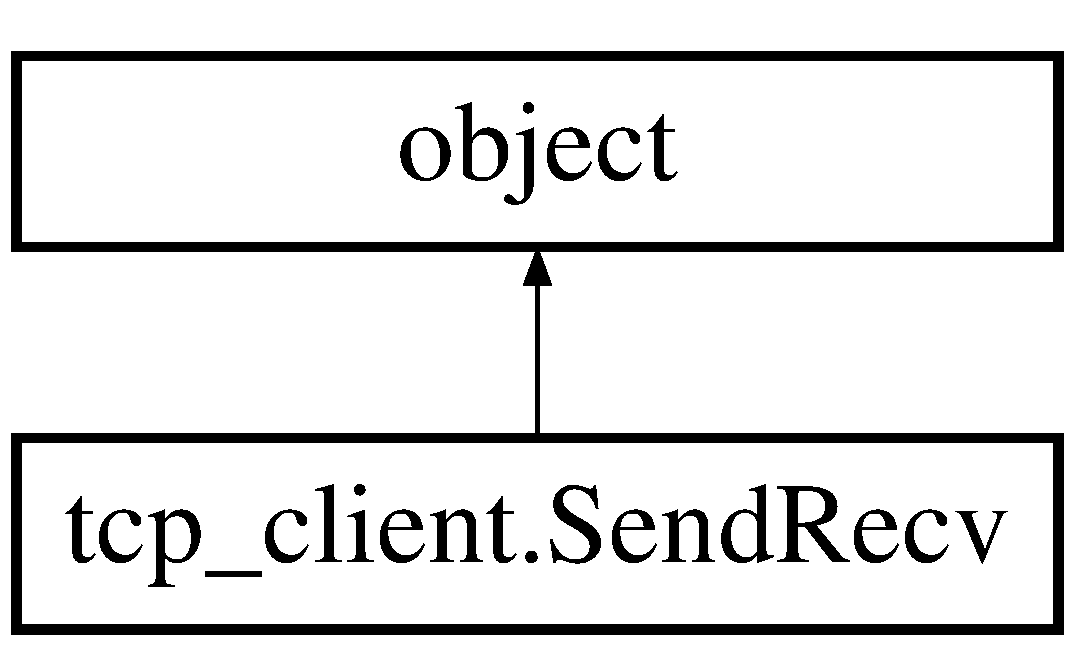
\includegraphics[height=2.000000cm]{classtcp__client_1_1_send_recv}
\end{center}
\end{figure}
\subsection*{Public Member Functions}
\begin{DoxyCompactItemize}
\item 
def \hyperlink{classtcp__client_1_1_send_recv_a6f93975d5740a905a785851f996ee9c7}{send\-\_\-single\-\_\-request}
\end{DoxyCompactItemize}


\subsection{Detailed Description}
\begin{DoxyVerb}This class handles a single request-response event.
\end{DoxyVerb}
 

\subsection{Member Function Documentation}
\hypertarget{classtcp__client_1_1_send_recv_a6f93975d5740a905a785851f996ee9c7}{\index{tcp\-\_\-client\-::\-Send\-Recv@{tcp\-\_\-client\-::\-Send\-Recv}!send\-\_\-single\-\_\-request@{send\-\_\-single\-\_\-request}}
\index{send\-\_\-single\-\_\-request@{send\-\_\-single\-\_\-request}!tcp_client::SendRecv@{tcp\-\_\-client\-::\-Send\-Recv}}
\subsubsection[{send\-\_\-single\-\_\-request}]{\setlength{\rightskip}{0pt plus 5cm}def tcp\-\_\-client.\-Send\-Recv.\-send\-\_\-single\-\_\-request (
\begin{DoxyParamCaption}
\item[{}]{self, }
\item[{}]{q, }
\item[{}]{waitlist, }
\item[{}]{sendlist, }
\item[{}]{event, }
\item[{}]{connections}
\end{DoxyParamCaption}
)}}\label{classtcp__client_1_1_send_recv_a6f93975d5740a905a785851f996ee9c7}


The documentation for this class was generated from the following file\-:\begin{DoxyCompactItemize}
\item 
\hyperlink{tcp__client_8py}{tcp\-\_\-client.\-py}\end{DoxyCompactItemize}

\hypertarget{classtcp__server_1_1_server}{\section{tcp\-\_\-server.\-Server Class Reference}
\label{classtcp__server_1_1_server}\index{tcp\-\_\-server.\-Server@{tcp\-\_\-server.\-Server}}
}
Inheritance diagram for tcp\-\_\-server.\-Server\-:\begin{figure}[H]
\begin{center}
\leavevmode
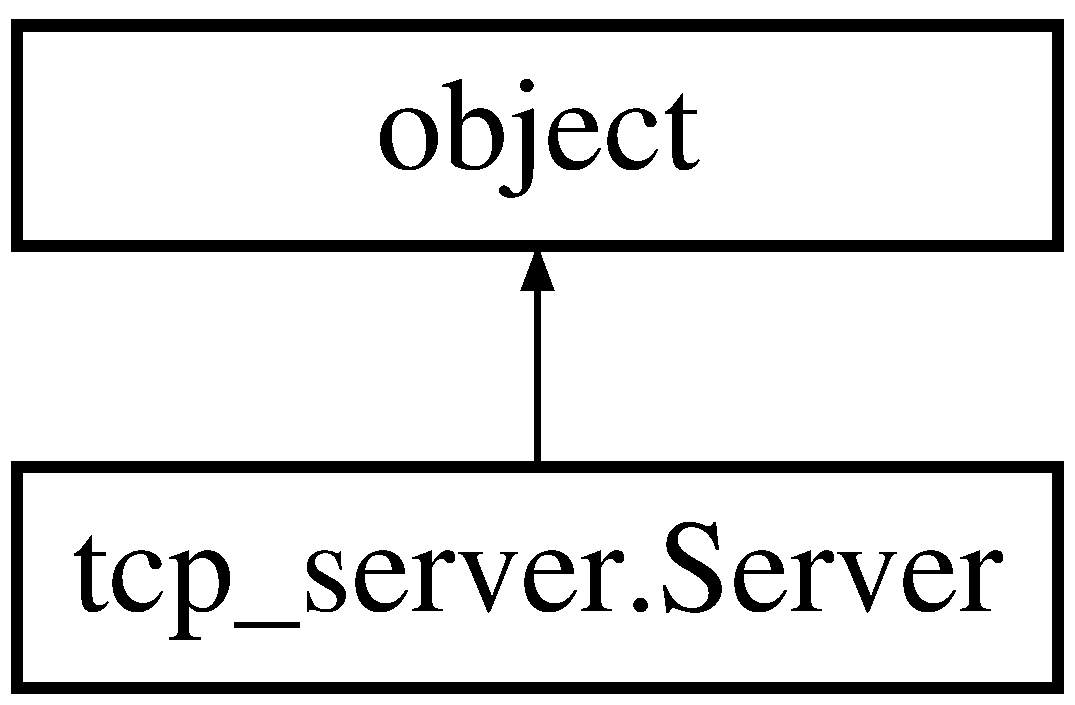
\includegraphics[height=2.000000cm]{classtcp__server_1_1_server}
\end{center}
\end{figure}
\subsection*{Public Member Functions}
\begin{DoxyCompactItemize}
\item 
def \hyperlink{classtcp__server_1_1_server_a708132c7505416c9b374d0b9013e8621}{\-\_\-\-\_\-init\-\_\-\-\_\-}
\item 
def \hyperlink{classtcp__server_1_1_server_a22124301cee8b0b1421354e4cea28481}{get\-\_\-port}
\item 
def \hyperlink{classtcp__server_1_1_server_a2a864226ef243124eec7b38ad5171513}{handle\-\_\-connection}
\item 
def \hyperlink{classtcp__server_1_1_server_a56aca41e09a8b0d0e05940d8b51111eb}{run\-\_\-socket\-\_\-server}
\end{DoxyCompactItemize}
\subsection*{Public Attributes}
\begin{DoxyCompactItemize}
\item 
\hyperlink{classtcp__server_1_1_server_aa0e56b6c0603c767cceb98a5ffda3f2d}{buffer\-\_\-size}
\end{DoxyCompactItemize}


\subsection{Constructor \& Destructor Documentation}
\hypertarget{classtcp__server_1_1_server_a708132c7505416c9b374d0b9013e8621}{\index{tcp\-\_\-server\-::\-Server@{tcp\-\_\-server\-::\-Server}!\-\_\-\-\_\-init\-\_\-\-\_\-@{\-\_\-\-\_\-init\-\_\-\-\_\-}}
\index{\-\_\-\-\_\-init\-\_\-\-\_\-@{\-\_\-\-\_\-init\-\_\-\-\_\-}!tcp_server::Server@{tcp\-\_\-server\-::\-Server}}
\subsubsection[{\-\_\-\-\_\-init\-\_\-\-\_\-}]{\setlength{\rightskip}{0pt plus 5cm}def tcp\-\_\-server.\-Server.\-\_\-\-\_\-init\-\_\-\-\_\- (
\begin{DoxyParamCaption}
\item[{}]{self, }
\item[{}]{host, }
\item[{}]{port = {\ttfamily None}, }
\item[{}]{buffer\-\_\-size = {\ttfamily 4096}}
\end{DoxyParamCaption}
)}}\label{classtcp__server_1_1_server_a708132c7505416c9b374d0b9013e8621}


\subsection{Member Function Documentation}
\hypertarget{classtcp__server_1_1_server_a22124301cee8b0b1421354e4cea28481}{\index{tcp\-\_\-server\-::\-Server@{tcp\-\_\-server\-::\-Server}!get\-\_\-port@{get\-\_\-port}}
\index{get\-\_\-port@{get\-\_\-port}!tcp_server::Server@{tcp\-\_\-server\-::\-Server}}
\subsubsection[{get\-\_\-port}]{\setlength{\rightskip}{0pt plus 5cm}def tcp\-\_\-server.\-Server.\-get\-\_\-port (
\begin{DoxyParamCaption}
\item[{}]{self}
\end{DoxyParamCaption}
)}}\label{classtcp__server_1_1_server_a22124301cee8b0b1421354e4cea28481}
\hypertarget{classtcp__server_1_1_server_a2a864226ef243124eec7b38ad5171513}{\index{tcp\-\_\-server\-::\-Server@{tcp\-\_\-server\-::\-Server}!handle\-\_\-connection@{handle\-\_\-connection}}
\index{handle\-\_\-connection@{handle\-\_\-connection}!tcp_server::Server@{tcp\-\_\-server\-::\-Server}}
\subsubsection[{handle\-\_\-connection}]{\setlength{\rightskip}{0pt plus 5cm}def tcp\-\_\-server.\-Server.\-handle\-\_\-connection (
\begin{DoxyParamCaption}
\item[{}]{self, }
\item[{}]{table, }
\item[{}]{connection, }
\item[{}]{client\-\_\-address}
\end{DoxyParamCaption}
)}}\label{classtcp__server_1_1_server_a2a864226ef243124eec7b38ad5171513}
\hypertarget{classtcp__server_1_1_server_a56aca41e09a8b0d0e05940d8b51111eb}{\index{tcp\-\_\-server\-::\-Server@{tcp\-\_\-server\-::\-Server}!run\-\_\-socket\-\_\-server@{run\-\_\-socket\-\_\-server}}
\index{run\-\_\-socket\-\_\-server@{run\-\_\-socket\-\_\-server}!tcp_server::Server@{tcp\-\_\-server\-::\-Server}}
\subsubsection[{run\-\_\-socket\-\_\-server}]{\setlength{\rightskip}{0pt plus 5cm}def tcp\-\_\-server.\-Server.\-run\-\_\-socket\-\_\-server (
\begin{DoxyParamCaption}
\item[{}]{self, }
\item[{}]{table, }
\item[{}]{expected\-\_\-conn\-\_\-num}
\end{DoxyParamCaption}
)}}\label{classtcp__server_1_1_server_a56aca41e09a8b0d0e05940d8b51111eb}


\subsection{Member Data Documentation}
\hypertarget{classtcp__server_1_1_server_aa0e56b6c0603c767cceb98a5ffda3f2d}{\index{tcp\-\_\-server\-::\-Server@{tcp\-\_\-server\-::\-Server}!buffer\-\_\-size@{buffer\-\_\-size}}
\index{buffer\-\_\-size@{buffer\-\_\-size}!tcp_server::Server@{tcp\-\_\-server\-::\-Server}}
\subsubsection[{buffer\-\_\-size}]{\setlength{\rightskip}{0pt plus 5cm}tcp\-\_\-server.\-Server.\-buffer\-\_\-size}}\label{classtcp__server_1_1_server_aa0e56b6c0603c767cceb98a5ffda3f2d}


The documentation for this class was generated from the following file\-:\begin{DoxyCompactItemize}
\item 
\hyperlink{tcp__server_8py}{tcp\-\_\-server.\-py}\end{DoxyCompactItemize}

\hypertarget{classpython__lib_1_1_singleton}{\section{python\-\_\-lib.\-Singleton Class Reference}
\label{classpython__lib_1_1_singleton}\index{python\-\_\-lib.\-Singleton@{python\-\_\-lib.\-Singleton}}
}
Inheritance diagram for python\-\_\-lib.\-Singleton\-:\begin{figure}[H]
\begin{center}
\leavevmode
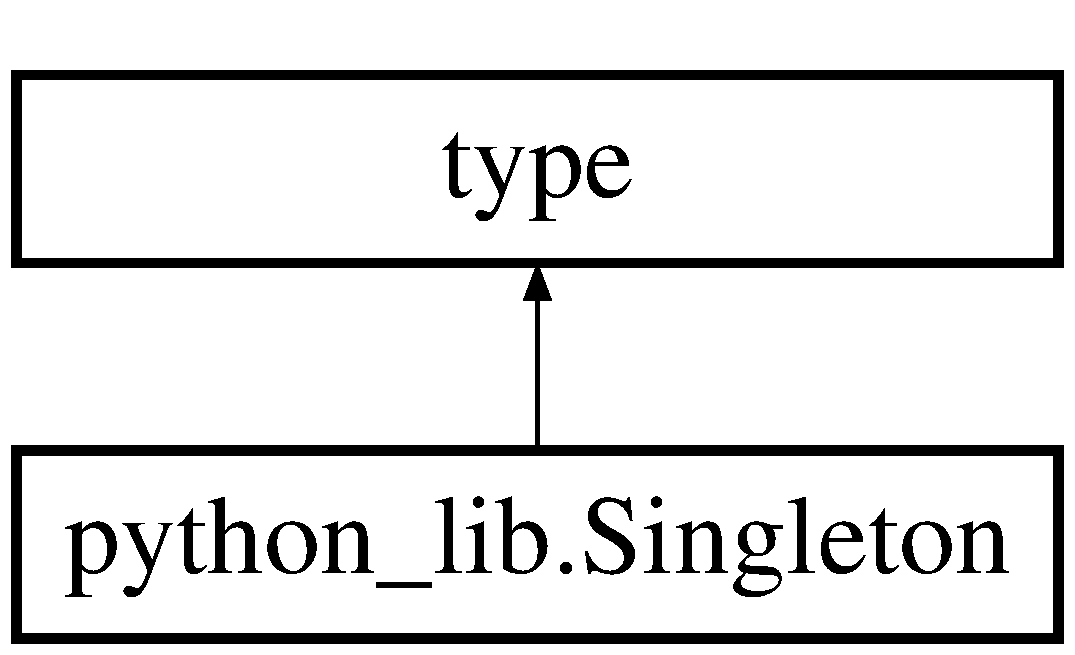
\includegraphics[height=2.000000cm]{classpython__lib_1_1_singleton}
\end{center}
\end{figure}
\subsection*{Public Member Functions}
\begin{DoxyCompactItemize}
\item 
def \hyperlink{classpython__lib_1_1_singleton_a7aabcae9e4bef6c7e77e5932204828d2}{\-\_\-\-\_\-call\-\_\-\-\_\-}
\end{DoxyCompactItemize}


\subsection{Member Function Documentation}
\hypertarget{classpython__lib_1_1_singleton_a7aabcae9e4bef6c7e77e5932204828d2}{\index{python\-\_\-lib\-::\-Singleton@{python\-\_\-lib\-::\-Singleton}!\-\_\-\-\_\-call\-\_\-\-\_\-@{\-\_\-\-\_\-call\-\_\-\-\_\-}}
\index{\-\_\-\-\_\-call\-\_\-\-\_\-@{\-\_\-\-\_\-call\-\_\-\-\_\-}!python_lib::Singleton@{python\-\_\-lib\-::\-Singleton}}
\subsubsection[{\-\_\-\-\_\-call\-\_\-\-\_\-}]{\setlength{\rightskip}{0pt plus 5cm}def python\-\_\-lib.\-Singleton.\-\_\-\-\_\-call\-\_\-\-\_\- (
\begin{DoxyParamCaption}
\item[{}]{cls, }
\item[{}]{args, }
\item[{}]{kwargs}
\end{DoxyParamCaption}
)}}\label{classpython__lib_1_1_singleton_a7aabcae9e4bef6c7e77e5932204828d2}


The documentation for this class was generated from the following file\-:\begin{DoxyCompactItemize}
\item 
\hyperlink{python__lib_8py}{python\-\_\-lib.\-py}\end{DoxyCompactItemize}

\hypertarget{classvpn__no__vpn_1_1tcpdump}{\section{vpn\-\_\-no\-\_\-vpn.\-tcpdump Class Reference}
\label{classvpn__no__vpn_1_1tcpdump}\index{vpn\-\_\-no\-\_\-vpn.\-tcpdump@{vpn\-\_\-no\-\_\-vpn.\-tcpdump}}
}
Inheritance diagram for vpn\-\_\-no\-\_\-vpn.\-tcpdump\-:\begin{figure}[H]
\begin{center}
\leavevmode
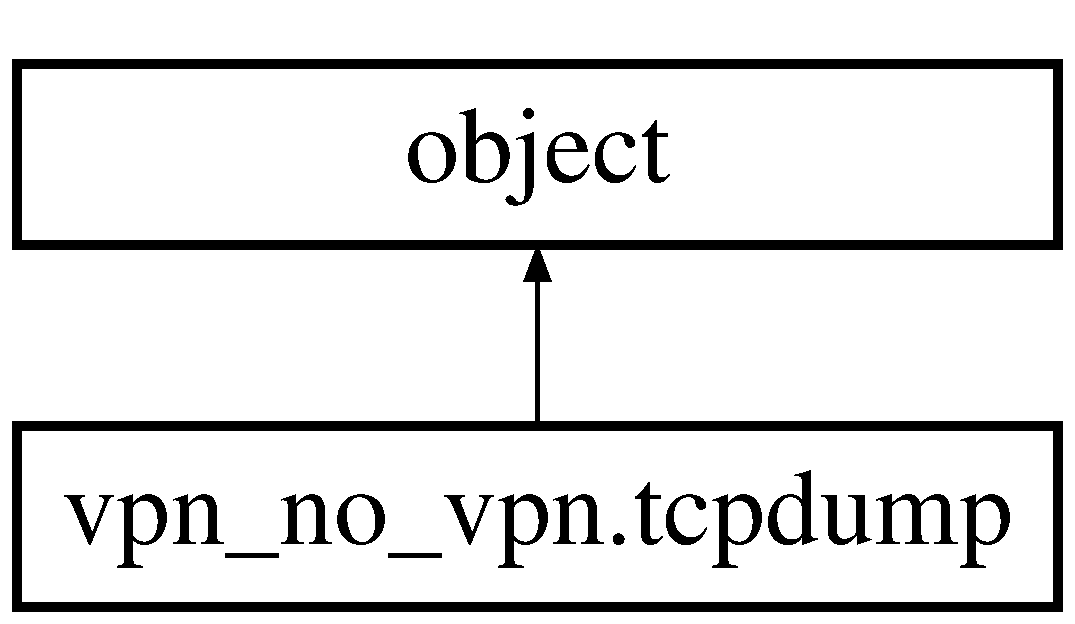
\includegraphics[height=2.000000cm]{classvpn__no__vpn_1_1tcpdump}
\end{center}
\end{figure}
\subsection*{Public Member Functions}
\begin{DoxyCompactItemize}
\item 
def \hyperlink{classvpn__no__vpn_1_1tcpdump_adf3771ce313acf6815feba172a08ef86}{\-\_\-\-\_\-init\-\_\-\-\_\-}
\item 
def \hyperlink{classvpn__no__vpn_1_1tcpdump_a674ed94aaa0da5c009e731d567a3386e}{start}
\item 
def \hyperlink{classvpn__no__vpn_1_1tcpdump_a6744565f0ca09e8f6ccbb99829d92175}{stop}
\item 
def \hyperlink{classvpn__no__vpn_1_1tcpdump_a31b222d9ee21e20677b24c397f7ede10}{status}
\end{DoxyCompactItemize}


\subsection{Constructor \& Destructor Documentation}
\hypertarget{classvpn__no__vpn_1_1tcpdump_adf3771ce313acf6815feba172a08ef86}{\index{vpn\-\_\-no\-\_\-vpn\-::tcpdump@{vpn\-\_\-no\-\_\-vpn\-::tcpdump}!\-\_\-\-\_\-init\-\_\-\-\_\-@{\-\_\-\-\_\-init\-\_\-\-\_\-}}
\index{\-\_\-\-\_\-init\-\_\-\-\_\-@{\-\_\-\-\_\-init\-\_\-\-\_\-}!vpn_no_vpn::tcpdump@{vpn\-\_\-no\-\_\-vpn\-::tcpdump}}
\subsubsection[{\-\_\-\-\_\-init\-\_\-\-\_\-}]{\setlength{\rightskip}{0pt plus 5cm}def vpn\-\_\-no\-\_\-vpn.\-tcpdump.\-\_\-\-\_\-init\-\_\-\-\_\- (
\begin{DoxyParamCaption}
\item[{}]{self, }
\item[{}]{dump\-\_\-name = {\ttfamily None}, }
\item[{}]{interface = {\ttfamily 'en0'}}
\end{DoxyParamCaption}
)}}\label{classvpn__no__vpn_1_1tcpdump_adf3771ce313acf6815feba172a08ef86}


\subsection{Member Function Documentation}
\hypertarget{classvpn__no__vpn_1_1tcpdump_a674ed94aaa0da5c009e731d567a3386e}{\index{vpn\-\_\-no\-\_\-vpn\-::tcpdump@{vpn\-\_\-no\-\_\-vpn\-::tcpdump}!start@{start}}
\index{start@{start}!vpn_no_vpn::tcpdump@{vpn\-\_\-no\-\_\-vpn\-::tcpdump}}
\subsubsection[{start}]{\setlength{\rightskip}{0pt plus 5cm}def vpn\-\_\-no\-\_\-vpn.\-tcpdump.\-start (
\begin{DoxyParamCaption}
\item[{}]{self}
\end{DoxyParamCaption}
)}}\label{classvpn__no__vpn_1_1tcpdump_a674ed94aaa0da5c009e731d567a3386e}
\hypertarget{classvpn__no__vpn_1_1tcpdump_a31b222d9ee21e20677b24c397f7ede10}{\index{vpn\-\_\-no\-\_\-vpn\-::tcpdump@{vpn\-\_\-no\-\_\-vpn\-::tcpdump}!status@{status}}
\index{status@{status}!vpn_no_vpn::tcpdump@{vpn\-\_\-no\-\_\-vpn\-::tcpdump}}
\subsubsection[{status}]{\setlength{\rightskip}{0pt plus 5cm}def vpn\-\_\-no\-\_\-vpn.\-tcpdump.\-status (
\begin{DoxyParamCaption}
\item[{}]{self}
\end{DoxyParamCaption}
)}}\label{classvpn__no__vpn_1_1tcpdump_a31b222d9ee21e20677b24c397f7ede10}
\hypertarget{classvpn__no__vpn_1_1tcpdump_a6744565f0ca09e8f6ccbb99829d92175}{\index{vpn\-\_\-no\-\_\-vpn\-::tcpdump@{vpn\-\_\-no\-\_\-vpn\-::tcpdump}!stop@{stop}}
\index{stop@{stop}!vpn_no_vpn::tcpdump@{vpn\-\_\-no\-\_\-vpn\-::tcpdump}}
\subsubsection[{stop}]{\setlength{\rightskip}{0pt plus 5cm}def vpn\-\_\-no\-\_\-vpn.\-tcpdump.\-stop (
\begin{DoxyParamCaption}
\item[{}]{self}
\end{DoxyParamCaption}
)}}\label{classvpn__no__vpn_1_1tcpdump_a6744565f0ca09e8f6ccbb99829d92175}


The documentation for this class was generated from the following file\-:\begin{DoxyCompactItemize}
\item 
\hyperlink{vpn__no__vpn_8py}{vpn\-\_\-no\-\_\-vpn.\-py}\end{DoxyCompactItemize}

\chapter{File Documentation}
\hypertarget{abbas__to__arash_8py}{\section{abbas\-\_\-to\-\_\-arash.\-py File Reference}
\label{abbas__to__arash_8py}\index{abbas\-\_\-to\-\_\-arash.\-py@{abbas\-\_\-to\-\_\-arash.\-py}}
}
\subsection*{Namespaces}
\begin{DoxyCompactItemize}
\item 
\hyperlink{namespaceabbas__to__arash}{abbas\-\_\-to\-\_\-arash}
\end{DoxyCompactItemize}
\subsection*{Functions}
\begin{DoxyCompactItemize}
\item 
def \hyperlink{namespaceabbas__to__arash_a6d1bc5ea921ec9271e6aa9259e04c34d}{abbas\-\_\-to\-\_\-arash.\-do\-\_\-one\-\_\-file}
\item 
def \hyperlink{namespaceabbas__to__arash_a91d8cb61c3815f7de34016ddde48d4e9}{abbas\-\_\-to\-\_\-arash.\-main}
\end{DoxyCompactItemize}

\hypertarget{abbas__to__arash2_8py}{\section{abbas\-\_\-to\-\_\-arash2.\-py File Reference}
\label{abbas__to__arash2_8py}\index{abbas\-\_\-to\-\_\-arash2.\-py@{abbas\-\_\-to\-\_\-arash2.\-py}}
}
\subsection*{Namespaces}
\begin{DoxyCompactItemize}
\item 
\hyperlink{namespaceabbas__to__arash2}{abbas\-\_\-to\-\_\-arash2}
\end{DoxyCompactItemize}
\subsection*{Functions}
\begin{DoxyCompactItemize}
\item 
def \hyperlink{namespaceabbas__to__arash2_a148667a787cd93b8faff2cb07624da4f}{abbas\-\_\-to\-\_\-arash2.\-do\-\_\-one\-\_\-file}
\item 
def \hyperlink{namespaceabbas__to__arash2_a9f39cd4dda65113f9e2b9b77a923b529}{abbas\-\_\-to\-\_\-arash2.\-main}
\end{DoxyCompactItemize}

\hypertarget{add__timestamp_8py}{\section{add\-\_\-timestamp.\-py File Reference}
\label{add__timestamp_8py}\index{add\-\_\-timestamp.\-py@{add\-\_\-timestamp.\-py}}
}
\subsection*{Namespaces}
\begin{DoxyCompactItemize}
\item 
\hyperlink{namespaceadd__timestamp}{add\-\_\-timestamp}
\end{DoxyCompactItemize}
\subsection*{Functions}
\begin{DoxyCompactItemize}
\item 
def \hyperlink{namespaceadd__timestamp_ac2bf9e3ea478f4ad61ca67022672e6b4}{add\-\_\-timestamp.\-main}
\end{DoxyCompactItemize}

\hypertarget{cdf_8py}{\section{cdf.\-py File Reference}
\label{cdf_8py}\index{cdf.\-py@{cdf.\-py}}
}
\subsection*{Classes}
\begin{DoxyCompactItemize}
\item 
class \hyperlink{classcdf_1_1_data_point}{cdf.\-Data\-Point}
\item 
class \hyperlink{classcdf_1_1_dump_stat}{cdf.\-Dump\-Stat}
\end{DoxyCompactItemize}
\subsection*{Namespaces}
\begin{DoxyCompactItemize}
\item 
\hyperlink{namespacecdf}{cdf}
\end{DoxyCompactItemize}
\subsection*{Functions}
\begin{DoxyCompactItemize}
\item 
def \hyperlink{namespacecdf_a860c68e20b4f59bbf288a8eea4016372}{cdf.\-dumpstat\-\_\-avg}
\item 
def \hyperlink{namespacecdf_afd91a77a1934a7fe3017b6b684c789d0}{cdf.\-parse\-\_\-output}
\item 
def \hyperlink{namespacecdf_a39ca068c3a42bbf3b662199607b75580}{cdf.\-run}
\item 
def \hyperlink{namespacecdf_ad7e6f86af33bf5afc8354e3ee95d2d84}{cdf.\-sorted\-\_\-list\-\_\-to\-\_\-cdf}
\item 
def \hyperlink{namespacecdf_a8163b6941e77518731e54fa703f671c2}{cdf.\-split\-\_\-list}
\item 
def \hyperlink{namespacecdf_a3c703da63dd8a0d11020ec6a644ed1cc}{cdf.\-do\-\_\-dir}
\item 
def \hyperlink{namespacecdf_ac60a4a166a9b445aa227e76918f38a35}{cdf.\-main}
\end{DoxyCompactItemize}

\hypertarget{compare__comms_8py}{\section{compare\-\_\-comms.\-py File Reference}
\label{compare__comms_8py}\index{compare\-\_\-comms.\-py@{compare\-\_\-comms.\-py}}
}
\subsection*{Namespaces}
\begin{DoxyCompactItemize}
\item 
\hyperlink{namespacecompare__comms}{compare\-\_\-comms}
\end{DoxyCompactItemize}
\subsection*{Functions}
\begin{DoxyCompactItemize}
\item 
def \hyperlink{namespacecompare__comms_a601e18a97e4d2ef71fba4b2066c38d80}{compare\-\_\-comms.\-read\-\_\-hex\-\_\-part}
\item 
def \hyperlink{namespacecompare__comms_aeb55d63b8ee3ed6eafa07319744d54c5}{compare\-\_\-comms.\-main}
\end{DoxyCompactItemize}

\hypertarget{excess__code_8py}{\section{excess\-\_\-code.\-py File Reference}
\label{excess__code_8py}\index{excess\-\_\-code.\-py@{excess\-\_\-code.\-py}}
}
\subsection*{Namespaces}
\begin{DoxyCompactItemize}
\item 
\hyperlink{namespaceexcess__code}{excess\-\_\-code}
\end{DoxyCompactItemize}
\subsection*{Functions}
\begin{DoxyCompactItemize}
\item 
def \hyperlink{namespaceexcess__code_a444ba0995cd870f581f9de7114587958}{excess\-\_\-code.\-read\-\_\-config\-\_\-file}
\item 
def \hyperlink{namespaceexcess__code_ad14739fab5c295bd8507c3fd0c455c95}{excess\-\_\-code.\-stream\-\_\-to\-\_\-queue2}
\end{DoxyCompactItemize}
\subsection*{Variables}
\begin{DoxyCompactItemize}
\item 
string \hyperlink{namespaceexcess__code_ad482d3963c307055389db29a0d9b9725}{excess\-\_\-code.\-ports\-\_\-pickle\-\_\-dump} = '-\/i /Users/arash/.ssh/ancsaaa-\/keypair\-\_\-ec2.\-pem ubuntu@72.\-44.\-56.\-209\-:/home/ubuntu/public\-\_\-html/free\-\_\-ports'
\item 
string \hyperlink{namespaceexcess__code_a7b2d2af5fa2f9fb9bf672bd07044add1}{excess\-\_\-code.\-host} = '72.\-44.\-56.\-209'
\item 
\hyperlink{namespaceexcess__code_ad9642f3ca12ca84caed8a65645ba6688}{excess\-\_\-code.\-queue} = q0+q1+q2+q3+q4
\item 
dictionary \hyperlink{namespaceexcess__code_ac888a34cdc4f20d89623cfe2f3b2727d}{excess\-\_\-code.\-table}
\end{DoxyCompactItemize}

\hypertarget{get__all__pairs_8py}{\section{get\-\_\-all\-\_\-pairs.\-py File Reference}
\label{get__all__pairs_8py}\index{get\-\_\-all\-\_\-pairs.\-py@{get\-\_\-all\-\_\-pairs.\-py}}
}
\subsection*{Namespaces}
\begin{DoxyCompactItemize}
\item 
\hyperlink{namespaceget__all__pairs}{get\-\_\-all\-\_\-pairs}
\end{DoxyCompactItemize}
\subsection*{Variables}
\begin{DoxyCompactItemize}
\item 
tuple \hyperlink{namespaceget__all__pairs_a1a098ebbb665e47d404618b95a8ea468}{get\-\_\-all\-\_\-pairs.\-follows\-\_\-dir} = os.\-path.\-abspath(follows\-\_\-dir)
\item 
tuple \hyperlink{namespaceget__all__pairs_ada0a4d6ed4e95218db6dcc5a8291b97a}{get\-\_\-all\-\_\-pairs.\-file\-\_\-list} = \hyperlink{namespacepython__lib_a32a11ff8ffaca42c9527412287edf0d5}{python\-\_\-lib.\-dir\-\_\-list}(follows\-\_\-dir, True)
\item 
list \hyperlink{namespaceget__all__pairs_a4c92b8a629bb4f726c383e672521eec4}{get\-\_\-all\-\_\-pairs.\-all\-\_\-pairs\-\_\-tshark} = \mbox{[}$\,$\mbox{]}
\item 
tuple \hyperlink{namespaceget__all__pairs_ab7236e4617b75a4400777ac08f262963}{get\-\_\-all\-\_\-pairs.\-f} = open(file, 'r')
\item 
tuple \hyperlink{namespaceget__all__pairs_a50bcbb8a8923b9dac536e87f54f29cce}{get\-\_\-all\-\_\-pairs.\-node0} = \hyperlink{namespacescapy__parser_ad232477d220b14b000fad3dac1d948a1}{scapy\-\_\-parser.\-convert\-\_\-ip}(((f.\-readline()).split()\mbox{[}2\mbox{]}).replace('\-:', '.'))
\item 
tuple \hyperlink{namespaceget__all__pairs_a8ac2e092f90c8fef4eddc9f665a71f51}{get\-\_\-all\-\_\-pairs.\-node1} = \hyperlink{namespacescapy__parser_ad232477d220b14b000fad3dac1d948a1}{scapy\-\_\-parser.\-convert\-\_\-ip}(((f.\-readline()).split()\mbox{[}2\mbox{]}).replace('\-:', '.'))
\item 
string \hyperlink{namespaceget__all__pairs_ab8b0605e707bec570403c17de2780a21}{get\-\_\-all\-\_\-pairs.\-c\-\_\-s\-\_\-pair} = '-\/'
\item 
tuple \hyperlink{namespaceget__all__pairs_ac36fe2b41b860b8d68de2dfc93945951}{get\-\_\-all\-\_\-pairs.\-l} = f.\-readline()
\item 
string \hyperlink{namespaceget__all__pairs_a15effa0696d56acc16b60bbf458e8b32}{get\-\_\-all\-\_\-pairs.\-command} = 'cp '
\item 
string \hyperlink{namespaceget__all__pairs_adbdf902a06dba3da9796b4676966b41b}{get\-\_\-all\-\_\-pairs.\-pickle\-\_\-dump} = pcap\-\_\-file+'\-\_\-all\-\_\-pairs'
\item 
tuple \hyperlink{namespaceget__all__pairs_a3a539e5269b6a98f445e695305ea7d7a}{get\-\_\-all\-\_\-pairs.\-all\-\_\-pairs\-\_\-scapy} = pickle.\-load(open(pickle\-\_\-dump, 'rb'))
\end{DoxyCompactItemize}

\hypertarget{ks2_8py}{\section{ks2.\-py File Reference}
\label{ks2_8py}\index{ks2.\-py@{ks2.\-py}}
}
\subsection*{Classes}
\begin{DoxyCompactItemize}
\item 
class \hyperlink{classks2_1_1_data_point}{ks2.\-Data\-Point}
\item 
class \hyperlink{classks2_1_1_dump_stat}{ks2.\-Dump\-Stat}
\end{DoxyCompactItemize}
\subsection*{Namespaces}
\begin{DoxyCompactItemize}
\item 
\hyperlink{namespaceks2}{ks2}
\end{DoxyCompactItemize}
\subsection*{Functions}
\begin{DoxyCompactItemize}
\item 
def \hyperlink{namespaceks2_a1f5bd5926d5beaa05f2964aa775914ff}{ks2.\-dumpstat\-\_\-avg}
\item 
def \hyperlink{namespaceks2_af9985767855e318b87d6d0a98e2598eb}{ks2.\-parse\-\_\-output}
\item 
def \hyperlink{namespaceks2_ae5fb7c0285ff12ec949e4f53d130f545}{ks2.\-run}
\item 
def \hyperlink{namespaceks2_af15630b152fbabcd3c5ea630557f64ae}{ks2.\-ks2}
\item 
def \hyperlink{namespaceks2_a5bedfd66ee1f9bf5e0f049208dd811fc}{ks2.\-split\-\_\-list}
\item 
def \hyperlink{namespaceks2_aec9fba868fd56ed1eae5920b4e8a15e0}{ks2.\-do\-\_\-dir}
\item 
def \hyperlink{namespaceks2_a6ad8dc5a3671d9ceb545b4d568683ffc}{ks2.\-main}
\end{DoxyCompactItemize}

\hypertarget{python__lib_8py}{\section{python\-\_\-lib.\-py File Reference}
\label{python__lib_8py}\index{python\-\_\-lib.\-py@{python\-\_\-lib.\-py}}
}
\subsection*{Classes}
\begin{DoxyCompactItemize}
\item 
class \hyperlink{classpython__lib_1_1_request_set}{python\-\_\-lib.\-Request\-Set}
\item 
class \hyperlink{classpython__lib_1_1_response_set}{python\-\_\-lib.\-Response\-Set}
\item 
class \hyperlink{classpython__lib_1_1_one_response}{python\-\_\-lib.\-One\-Response}
\item 
class \hyperlink{classpython__lib_1_1_singleton}{python\-\_\-lib.\-Singleton}
\item 
class \hyperlink{classpython__lib_1_1_configs}{python\-\_\-lib.\-Configs}
\item 
class \hyperlink{classpython__lib_1_1_instance}{python\-\_\-lib.\-Instance}
\end{DoxyCompactItemize}
\subsection*{Namespaces}
\begin{DoxyCompactItemize}
\item 
\hyperlink{namespacepython__lib}{python\-\_\-lib}
\end{DoxyCompactItemize}
\subsection*{Functions}
\begin{DoxyCompactItemize}
\item 
def \hyperlink{namespacepython__lib_a7773c2422730b63639dd7dca2ab1c496}{python\-\_\-lib.\-P\-R\-I\-N\-T\-\_\-\-A\-C\-T\-I\-O\-N}
\item 
def \hyperlink{namespacepython__lib_a097b0a877da08c723a02d07c0cb4cb57}{python\-\_\-lib.\-read\-\_\-args}
\item 
def \hyperlink{namespacepython__lib_adacb0c96f7321a6b040892a22e4cbdc9}{python\-\_\-lib.\-append\-\_\-to\-\_\-file}
\item 
def \hyperlink{namespacepython__lib_a32a11ff8ffaca42c9527412287edf0d5}{python\-\_\-lib.\-dir\-\_\-list}
\end{DoxyCompactItemize}

\hypertarget{scapy__parser_8py}{\section{scapy\-\_\-parser.\-py File Reference}
\label{scapy__parser_8py}\index{scapy\-\_\-parser.\-py@{scapy\-\_\-parser.\-py}}
}
\subsection*{Namespaces}
\begin{DoxyCompactItemize}
\item 
\hyperlink{namespacescapy__parser}{scapy\-\_\-parser}
\end{DoxyCompactItemize}
\subsection*{Functions}
\begin{DoxyCompactItemize}
\item 
def \hyperlink{namespacescapy__parser_afe4115215cb92dd83c69c093ca1dc39c}{scapy\-\_\-parser.\-read\-\_\-packet\-\_\-file}
\item 
def \hyperlink{namespacescapy__parser_a8380a4cd72a24b37c31aa940f9e46ca8}{scapy\-\_\-parser.\-stream\-\_\-to\-\_\-queue}
\item 
def \hyperlink{namespacescapy__parser_ab235f32be59c5d52d6a4741e261b48ec}{scapy\-\_\-parser.\-map\-\_\-follows}
\item 
def \hyperlink{namespacescapy__parser_ad232477d220b14b000fad3dac1d948a1}{scapy\-\_\-parser.\-convert\-\_\-ip}
\item 
def \hyperlink{namespacescapy__parser_ad297d10c555e7fbcfccf73cee8e38256}{scapy\-\_\-parser.\-read\-\_\-payload}
\item 
def \hyperlink{namespacescapy__parser_a402e671cc2705b00b5f66d9b3dd57f34}{scapy\-\_\-parser.\-create\-\_\-packets\-\_\-file}
\item 
def \hyperlink{namespacescapy__parser_a907496fe847749d57c9e2f07359b4ccc}{scapy\-\_\-parser.\-sanity\-\_\-check}
\item 
def \hyperlink{namespacescapy__parser_a91451a1858fe0e45095ea130b7fa0165}{scapy\-\_\-parser.\-do\-\_\-tshark\-\_\-follows}
\item 
def \hyperlink{namespacescapy__parser_a64e52994b8f6fd553cdaa44b2047f61c}{scapy\-\_\-parser.\-read\-\_\-client\-\_\-ip}
\item 
def \hyperlink{namespacescapy__parser_a5f96040fae556e80468aae165afaf565}{scapy\-\_\-parser.\-main}
\end{DoxyCompactItemize}
\subsection*{Variables}
\begin{DoxyCompactItemize}
\item 
\hyperlink{namespacescapy__parser_ab5c773d1946dd024ca6f829ba3354d2d}{scapy\-\_\-parser.\-D\-E\-B\-U\-G0} = False
\end{DoxyCompactItemize}

\hypertarget{tcp__client_8py}{\section{tcp\-\_\-client.\-py File Reference}
\label{tcp__client_8py}\index{tcp\-\_\-client.\-py@{tcp\-\_\-client.\-py}}
}
\subsection*{Classes}
\begin{DoxyCompactItemize}
\item 
class \hyperlink{classtcp__client_1_1_connections}{tcp\-\_\-client.\-Connections}
\item 
class \hyperlink{classtcp__client_1_1_send_recv}{tcp\-\_\-client.\-Send\-Recv}
\item 
class \hyperlink{classtcp__client_1_1_queue}{tcp\-\_\-client.\-Queue}
\end{DoxyCompactItemize}
\subsection*{Namespaces}
\begin{DoxyCompactItemize}
\item 
\hyperlink{namespacetcp__client}{tcp\-\_\-client}
\end{DoxyCompactItemize}
\subsection*{Functions}
\begin{DoxyCompactItemize}
\item 
def \hyperlink{namespacetcp__client_ab399fb69cbd86776bbd54e12f5bb3310}{tcp\-\_\-client.\-read\-\_\-ports}
\item 
def \hyperlink{namespacetcp__client_a619d86369bc1818130dc4bdafe33a122}{tcp\-\_\-client.\-run}
\item 
def \hyperlink{namespacetcp__client_aeeaf345aad4737e78cab8295d4b0fc9b}{tcp\-\_\-client.\-main}
\end{DoxyCompactItemize}
\subsection*{Variables}
\begin{DoxyCompactItemize}
\item 
\hyperlink{namespacetcp__client_a895ed640f9bf5e6fa45e32d6851fd3ec}{tcp\-\_\-client.\-D\-E\-B\-U\-G0} = False
\end{DoxyCompactItemize}

\hypertarget{tcp__server_8py}{\section{tcp\-\_\-server.\-py File Reference}
\label{tcp__server_8py}\index{tcp\-\_\-server.\-py@{tcp\-\_\-server.\-py}}
}
\subsection*{Classes}
\begin{DoxyCompactItemize}
\item 
class \hyperlink{classtcp__server_1_1_server}{tcp\-\_\-server.\-Server}
\end{DoxyCompactItemize}
\subsection*{Namespaces}
\begin{DoxyCompactItemize}
\item 
\hyperlink{namespacetcp__server}{tcp\-\_\-server}
\end{DoxyCompactItemize}
\subsection*{Functions}
\begin{DoxyCompactItemize}
\item 
def \hyperlink{namespacetcp__server_a345a4bad31f0a853442880183b510ddc}{tcp\-\_\-server.\-read\-\_\-c\-\_\-s\-\_\-pair\-\_\-to\-\_\-port}
\item 
def \hyperlink{namespacetcp__server_a9a4d4bee3a12f34288c4cc517ccf9976}{tcp\-\_\-server.\-run}
\item 
def \hyperlink{namespacetcp__server_ad7647812bebfb857f5c583aad72f6c4f}{tcp\-\_\-server.\-main}
\end{DoxyCompactItemize}
\subsection*{Variables}
\begin{DoxyCompactItemize}
\item 
int \hyperlink{namespacetcp__server_a50c596f6928f69e658be5f1677233f96}{tcp\-\_\-server.\-D\-E\-B\-U\-G} = 2
\end{DoxyCompactItemize}

\hypertarget{template_8py}{\section{template.\-py File Reference}
\label{template_8py}\index{template.\-py@{template.\-py}}
}
\subsection*{Namespaces}
\begin{DoxyCompactItemize}
\item 
\hyperlink{namespacetemplate}{template}
\end{DoxyCompactItemize}
\subsection*{Functions}
\begin{DoxyCompactItemize}
\item 
def \hyperlink{namespacetemplate_a0c2b50f0e7a34ce1ceec58642be5a060}{template.\-run}
\item 
def \hyperlink{namespacetemplate_ae00dac90929f3c1ab18c6056867b7074}{template.\-main}
\end{DoxyCompactItemize}

\hypertarget{throuput__tshark_8py}{\section{throuput\-\_\-tshark.\-py File Reference}
\label{throuput__tshark_8py}\index{throuput\-\_\-tshark.\-py@{throuput\-\_\-tshark.\-py}}
}
\subsection*{Classes}
\begin{DoxyCompactItemize}
\item 
class \hyperlink{classthrouput__tshark_1_1_data_point}{throuput\-\_\-tshark.\-Data\-Point}
\item 
class \hyperlink{classthrouput__tshark_1_1_dump_stat}{throuput\-\_\-tshark.\-Dump\-Stat}
\end{DoxyCompactItemize}
\subsection*{Namespaces}
\begin{DoxyCompactItemize}
\item 
\hyperlink{namespacethrouput__tshark}{throuput\-\_\-tshark}
\end{DoxyCompactItemize}
\subsection*{Functions}
\begin{DoxyCompactItemize}
\item 
def \hyperlink{namespacethrouput__tshark_a7cf943f2dc4fd029521106818dc6f42c}{throuput\-\_\-tshark.\-dumpstat\-\_\-avg}
\item 
def \hyperlink{namespacethrouput__tshark_aadae1a38443951d84893a766c7544c4e}{throuput\-\_\-tshark.\-parse\-\_\-output}
\item 
def \hyperlink{namespacethrouput__tshark_ad87e88509990133de6a38df4742dc876}{throuput\-\_\-tshark.\-run}
\item 
def \hyperlink{namespacethrouput__tshark_ab46319be4c40947f3596aee776407a83}{throuput\-\_\-tshark.\-split\-\_\-list}
\item 
def \hyperlink{namespacethrouput__tshark_a61c2eee9729017b8321509878cca8153}{throuput\-\_\-tshark.\-do\-\_\-dir}
\item 
def \hyperlink{namespacethrouput__tshark_a37360c9b79c8d4a0bc29f07bf195a3b2}{throuput\-\_\-tshark.\-main}
\end{DoxyCompactItemize}

\hypertarget{tornado__server_8py}{\section{tornado\-\_\-server.\-py File Reference}
\label{tornado__server_8py}\index{tornado\-\_\-server.\-py@{tornado\-\_\-server.\-py}}
}
\subsection*{Classes}
\begin{DoxyCompactItemize}
\item 
class \hyperlink{classtornado__server_1_1_main_handler}{tornado\-\_\-server.\-Main\-Handler}
\item 
class \hyperlink{classtornado__server_1_1_record_replay}{tornado\-\_\-server.\-Record\-Replay}
\item 
class \hyperlink{classtornado__server_1_1_re_run}{tornado\-\_\-server.\-Re\-Run}
\end{DoxyCompactItemize}
\subsection*{Namespaces}
\begin{DoxyCompactItemize}
\item 
\hyperlink{namespacetornado__server}{tornado\-\_\-server}
\end{DoxyCompactItemize}
\subsection*{Functions}
\begin{DoxyCompactItemize}
\item 
def \hyperlink{namespacetornado__server_af5c4e1dbe49ac1fd487f7a81d88d90ff}{tornado\-\_\-server.\-print\-\_\-req\-\_\-details}
\item 
def \hyperlink{namespacetornado__server_aba1ab110c678f99f71be9ab9423398f4}{tornado\-\_\-server.\-print\-\_\-req\-\_\-headers}
\item 
def \hyperlink{namespacetornado__server_a67086ec0246941bad1dcd70e34bf7cb8}{tornado\-\_\-server.\-pid\-\_\-status}
\item 
def \hyperlink{namespacetornado__server_af4c6404a74c334144a579fb9a158f3c7}{tornado\-\_\-server.\-main}
\end{DoxyCompactItemize}

\hypertarget{vpn__no__vpn_8py}{\section{vpn\-\_\-no\-\_\-vpn.\-py File Reference}
\label{vpn__no__vpn_8py}\index{vpn\-\_\-no\-\_\-vpn.\-py@{vpn\-\_\-no\-\_\-vpn.\-py}}
}
\subsection*{Classes}
\begin{DoxyCompactItemize}
\item 
class \hyperlink{classvpn__no__vpn_1_1tcpdump}{vpn\-\_\-no\-\_\-vpn.\-tcpdump}
\end{DoxyCompactItemize}
\subsection*{Namespaces}
\begin{DoxyCompactItemize}
\item 
\hyperlink{namespacevpn__no__vpn}{vpn\-\_\-no\-\_\-vpn}
\end{DoxyCompactItemize}
\subsection*{Functions}
\begin{DoxyCompactItemize}
\item 
def \hyperlink{namespacevpn__no__vpn_a1119e982dc3f687c8bb0edb1e9953354}{vpn\-\_\-no\-\_\-vpn.\-meddle\-\_\-vpn}
\item 
def \hyperlink{namespacevpn__no__vpn_a4da84311848fe51d8b56d51c475b4291}{vpn\-\_\-no\-\_\-vpn.\-run\-\_\-one}
\item 
def \hyperlink{namespacevpn__no__vpn_a31941e50267268cccab158e35a4e7fde}{vpn\-\_\-no\-\_\-vpn.\-main}
\end{DoxyCompactItemize}

\hypertarget{wrapper__client_8py}{\section{wrapper\-\_\-client.\-py File Reference}
\label{wrapper__client_8py}\index{wrapper\-\_\-client.\-py@{wrapper\-\_\-client.\-py}}
}
\subsection*{Namespaces}
\begin{DoxyCompactItemize}
\item 
\hyperlink{namespacewrapper__client}{wrapper\-\_\-client}
\end{DoxyCompactItemize}
\subsection*{Functions}
\begin{DoxyCompactItemize}
\item 
def \hyperlink{namespacewrapper__client_a33b0936c83fc1c21379c1dd74be11bda}{wrapper\-\_\-client.\-main}
\end{DoxyCompactItemize}

\hypertarget{wrapper__server_8py}{\section{wrapper\-\_\-server.\-py File Reference}
\label{wrapper__server_8py}\index{wrapper\-\_\-server.\-py@{wrapper\-\_\-server.\-py}}
}
\subsection*{Namespaces}
\begin{DoxyCompactItemize}
\item 
\hyperlink{namespacewrapper__server}{wrapper\-\_\-server}
\end{DoxyCompactItemize}
\subsection*{Functions}
\begin{DoxyCompactItemize}
\item 
def \hyperlink{namespacewrapper__server_adb1220df41301f0949da5f381761f139}{wrapper\-\_\-server.\-do\-\_\-all}
\item 
def \hyperlink{namespacewrapper__server_abec04fa71a16c5b7305dc48b8fcaca33}{wrapper\-\_\-server.\-main}
\end{DoxyCompactItemize}

%--- End generated contents ---

% Index
\newpage
\phantomsection
\addcontentsline{toc}{part}{Index}
\printindex

\end{document}
